%
% Stanford University PhD thesis style -- modifications to the report style
% This is unofficial so you should always double check against the
% Registrar's office rules
% See http://library.stanford.edu/research/bibliography-management/latex-and-bibtex
% 
% Example of use below
% See the suthesis-2e.sty file for documentation
%

\documentclass{report}
\usepackage{suthesis-2e}

\usepackage{amsmath}
\usepackage{amssymb}
\usepackage{booktabs}
\usepackage{graphicx}
\usepackage{hyperref}

\usepackage[numbered]{algorithm}
\usepackage[noend]{algorithmic}
\usepackage[super]{nth}

\floatstyle{boxed}
\newfloat{Listing}{t}{ext}
\renewcommand{\algorithmicrequire}{\small\textbf{Input:}}
\renewcommand{\algorithmicensure}{\small\textbf{Output:}}

\DeclareMathOperator*{\argmin}{arg\,min}
\DeclareMathOperator*{\argmax}{arg\,max}

\begin{document}

\newcommand{\shortcite}[1]{\cite{#1}}

\title{Trajectory Optimization Methods for Drone Cameras}
\author{Mike Roberts}
\dept{Computer Science}
\principaladviser{Pat Hanrahan}
\firstreader{Doug James}
\secondreader{Fredo Durand}
%\thirdreader{Fredo Durand} %if needed
%\fourthreader{Severus Snape} %if needed

\beforepreface

\prefacesection{Acknowledgments}

This dissertation would have been impossible without the help and support of many people.
I am indebted to all of you, and I am delighted to take this opportunity to recognize the positive impact that all of you have had on my life.

I want to begin by thanking the world's greatest advisor, Pat Hanrahan.
You took me on as your student even though I didn't know what I was doing.
You were so patient with me, and you gave me the time I needed to grow into a good student and an independent researcher.
You gave me the freedom to choose my own research directions.
You spent countless hours with me discussing research ideas, and you provided a seemingly endless supply of helpful feedback on paper drafts and talks.
Your guidance and mentorship have been transformative.

I want to thank Fr{\'e}do Durand and Doug James for serving on my dissertation reading committee.
Fr{\'e}do's notes on writing became my bible during my graduate studies, and I especially appreciate the advice Doug gave me about choosing research problems back at Harvard.
Doug and Fr{\'e}do also provided very helpful and detailed feedback on an early version of my job talk. I want to thank Ron Fedkiw and Stephen Boyd for serving on my dissertation defense committee.
Ron's lab was an intellectual home-away-from-home, and I especially enjoyed all of our lively discussions over the years.
I also heard a rumor that Ron rescued my Stanford application from the reject pile -- thank you.
Stephen's textbooks, classes, online lectures, and office hours were always incredibly educational, both in their substance and style.

I want to thank Hanspeter Pfister.
You were the first person to give me a chance to do research outside my home town.
This opportunity changed my life.
I also want to thank John Owens.
You were the first person I ever met at an academic conference, and have been an exemplary role model and continuing source of inspiration ever since.
I especially appreciate your guidance on re-applying to Stanford, which undoubtedly changed my life for the better.
While you were hosting me for a visit at UC Davis, Shubho Sengupta offered a comfy couch to sleep on, and Andrew Davidson gave me a lift to the airport -- thank you.

I want to thank my recommenders:
Adam Finkelstein, Pat Hanrahan, Doug James, John Owens, Hanspeter Pfister, and Sudipta Sinha.
You all submitted a gazillion recommendation letters on my behalf, and were all so incredibly generous with your time.
Discussing research ideas with Adam was always fun and inspirational.
Sudipta introduced me to submodular functions, which had a big impact on this dissertation, and our whiteboard sessions were some of my favorite experiences in graduate school.

During my time at Stanford, I benefited from many other amazing mentors.
Floraine Berthouzoz was an incredible role model and collaborator.
Our discussions were always fun and inspirational, and our late-night paper editing sessions had a lasting impact on me.
I wish I could have shared more of the ideas in this dissertation with you.
Russ Tedrake carefully replied to so many of my emails, and his online lectures inspired much of the work in this dissertation.
Stefanie Jegelka's tutorials and online lectures also directly inspired the work in this dissertation.
Mykel Kochenderfer and Silvio Savarese agreed to participate in my qualifying exam -- thank you.
Vladlen Koltun and Ge Wang agreed to take me on as a rotation student even though I didn't know what I was doing.
Maneesh Agrawala, Michael Bernstein, Kayvon Fatahalian, Doug James, James Landay, and Mac Schwager provided valuable ongoing advice, and were all extremely generous with their time.
Wilmot Li provided detailed and helpful feedback on an early paper draft.
Working with John Owens and David Luebke at Udacity was a once-in-a-lifetime opportunity.
Working closely with Frank Dellaert at Skydio was incredibly fun and educational.
Debadeepta Dey, Neel Joshi, Ashish Kapoor, Shital Shah, and Sudipta Sinha at Microsoft Research were all fantastic collaborators.

I couldn't have asked for better friends, colleagues, and labmates at Stanford.
Niels Joubert immediately became a close collaborator and an even closer friend.
Indeed, many of the ideas in this dissertation were conceived during our memorable late-night coding sessions.
Anh Truong and Jane E quickly became trusted confidants and valued collaborators.
I especially appreciate all of Anh's fantastic work on our 3D scanning project, and Jane's work to narrate one of our supplementary videos.
Gilbert Bernstein, Zach DeVito, James Hegarty, Matt Fisher, Sharon Lin, Jonathan Ragan-Kelley, Daniel Ritchie, Manolis Savva, Lingfeng Yang, and Yi-Ting Yeh were fantastic colleagues and role models.
I especially want to thank Zach and Jonathan for putting up with it when I would sleep in their office -- you were doing me a bigger favor than you realize.
Ross Daly and Mackenzie Leake helped to prepare figures and supplementary materials for a paper at the last possible nanosecond.
Maxine Lim created several figures that appear in this dissertation.
Ali Alkhatib, Will Crichton, Abe Davis, Jingyi Li, Alex Poms, and Jerry Talton provided a ton of helpful feedback on various talks and paper drafts.
I especially appreciated all the conversations, coding sessions, and late-night snacks with Ed Quigley and Winnie Lin.
Justin Johnson was the world's greatest group project partner -- thank you for being so patient with me.
Enzo Busseti and Okke Schrijvers became life-long friends.

I also had the opportunity to work with many wonderful friends, colleagues, and labmates at Harvard.
Won-Ki Jeong was willing to work with me even though I didn't know what I was doing.
Bjoern Andres, Verena Kaynig-Fittkau, and Amelio Vazquez-Reina inspired me to learn everything I could about optimization.
Moritz Baecher, Kevin Dale, Kalyan Sunkavalli, and Justin Thaler became close friends.
I especially want to thank Kevin and Kalyan for generously sharing their accommodations at SIGGRAPH with me -- you were doing me a bigger favor than you realize.  
Johanna Beyer, Nicolas Bonneel, Michelle Borkin, Cris Cecka, Markus Hadwiger, Daniel Haehn, Ray Jones, Bobby Kasthuri, Seymour Knowles-Barley,  Jeff Lichtman, Miriah Meyer, Nicolas Pinto, and Amanda Randles were wonderful collaborators and role models.

I appreciate the technical and administrative support I received throughout my graduate studies.
Weichao Qiu provided extensive technical support with his incredibly useful UnrealCV Python library.
Jim Piavis and Ross Robinson provided valuable expertise as safety pilots, and Don Gillett granted us permission to 3D scan his barn.
I am also thankful for the support I received from the exceptional administrative staff in the Stanford Computer Science Department.
In particular, Helen Buendicho, Chris Downey, Jam Kiattinant, Andrea Kuduk, Jillian Lentz, Monica Niemiec, and Jay Subramanian have all gone out of their way to help me countless times.

The work in this dissertation was funded by NSERC and a generous grant from Google.
3DRobotics generously donated the drone hardware we used throughout this dissertation, and granted us permission to 3D scan their industrial scene.
Thank you.

Moving beyond academia, I am grateful for the people in my personal life that have helped and supported me throughout my graduate career.
In Calgary, Chelsea Leishman and the rest of Leishman family always believed in me.
Rob Faust remains a life-long friend, and is still the best DJ partner on the planet.
In Boston, Eric Baczuk and Simon Scheider were always great workout buddies, and I always enjoyed our endless conversations at Chipotle.
When I got to Stanford, I was fortunate to navigate the challenges and adventures of graduate student life alongside Okke Schrijvers.
Shannon Hoban and the rest of the Hoban family, Danielle Radin, Nikil and Tara Viswanathan, Ian Winters, and Brooke Wright all helped to make Stanford feel like home.
Dinner parties with Greg Benedict and Leah Meth were always welcome study breaks.
Cedar House in Berkeley was a home-away-from-home, and Iris Corey, Hannah Marshall, and Armin Samii immediately became close friends.
I especially appreciate Armin for hosting me when I was considering attending UC Berkeley for graduate school, and I want to thank Armin and Dave Jackson for lending me their spare hotel room at SIGGRAPH.

Throughout my graduate studies, I had the opportunity to meet many wonderful housemates.
In particular, Heather and Zac Altman, Katie Ballenger, Caroline Beaudon, Akhila Bettadapur, Nigel Kooreman, Felipe Pincheira, Jessica Schrouff, Gustavo Schwenkler, Alex and Andreas Zoellner quickly became close friends, and all made the Hackmann House a joy to come home to.
Living in the Facebook House was surreal and hilarious thanks to Kai Kuspa.
I was extremely fortunate to live in Hawthorne Manor with  Aladin Corhodzic, Mike D'Amico, Sherif Kassatly, and Ibrahim Toukan.
I experienced so many laughs and wonderful memories with all of you.
I especially appreciate Sherif and Ibrahim for lending me a couple of months of rent at one point -- thank you.
Sherif also did me a huge favor by lending me his old laptop when mine got stolen.

My time at Stanford was undoubtedly more fun because of all the opportunities I had to get in my musical happy place through DJing.
I am thankful for all my friends that made this possible.
Armin Samii hosted the best house party of all time, and trusted me to DJ at it.
Jack Wang at KZSU trusted me to DJ at Stanford football games soon after we met.
Jake Zeller went out of his way to connect me with nightclubs in San Francisco, which ultimately enabled me to open for the Chainsmokers.
Working with Ladidi Gharba was a once-in-a-lifetime opportunity.
I miss you.
Henrik Thorenfeldt trusted me to DJ at the Young Scandinavians Club cabin at Clear Lake.
We quickly became close friends, and Clear Lake became a second family.
Brian Mac immediately became a close friend and trusted DJ partner.

Finally, I want to thank my mom and dad, Judy and Rodger Roberts, for their kind words of support over the years.
And I especially want to thank my brother, Anthony Roberts.
Several times throughout my studies, you loaned me a significant amount of money, and these extraordinary acts of trust enabled me to continue pushing forward.
I would not have been able to complete this dissertation without you.
Thank you.

\prefacesection{Acknowledgments}

This dissertation would have been impossible without the help and support of many people.
I am indebted to all of you, and I am delighted to take this opportunity to recognize the positive impact that all of you have had on my life.

I want to begin by thanking the world's greatest advisor, Pat Hanrahan.
You took me on as your student even though I didn't know what I was doing.
You were so patient with me, and you gave me the time I needed to grow into a good student and an independent researcher.
You gave me the freedom to choose my own research directions.
You spent countless hours with me discussing research ideas, and you provided a seemingly endless supply of helpful feedback on paper drafts and talks.
Your guidance and mentorship have been transformative.

I want to thank Fr{\'e}do Durand and Doug James for serving on my dissertation reading committee.
Fr{\'e}do's notes on writing became my bible during my graduate studies, and I especially appreciate the advice Doug gave me about choosing research problems back at Harvard.
Doug and Fr{\'e}do also provided very helpful and detailed feedback on an early version of my job talk. I want to thank Ron Fedkiw and Stephen Boyd for serving on my dissertation defense committee.
Ron's lab was an intellectual home-away-from-home, and I especially enjoyed all of our lively discussions over the years.
I also heard a rumor that Ron rescued my Stanford application from the reject pile -- thank you.
Stephen's textbooks, classes, online lectures, and office hours were always incredibly educational, both in their substance and style.

I want to thank Hanspeter Pfister.
You were the first person to give me a chance to do research outside my home town.
This opportunity changed my life.
I also want to thank John Owens.
You were the first person I ever met at an academic conference, and have been an exemplary role model and continuing source of inspiration ever since.
I especially appreciate your guidance on re-applying to Stanford, which undoubtedly changed my life for the better.
While you were hosting me for a visit at UC Davis, Shubho Sengupta offered a comfy couch to sleep on, and Andrew Davidson gave me a lift to the airport -- thank you.

I want to thank my recommenders:
Adam Finkelstein, Pat Hanrahan, Doug James, John Owens, Hanspeter Pfister, and Sudipta Sinha.
You all submitted a gazillion recommendation letters on my behalf, and were all so incredibly generous with your time.
Discussing research ideas with Adam was always fun and inspirational.
Sudipta introduced me to submodular functions, which had a big impact on this dissertation, and our whiteboard sessions were some of my favorite experiences in graduate school.

During my time at Stanford, I benefited from many other amazing mentors.
Floraine Berthouzoz was an incredible role model and collaborator.
Our discussions were always fun and inspirational, and our late-night paper editing sessions had a lasting impact on me.
I wish I could have shared more of the ideas in this dissertation with you.
Russ Tedrake carefully replied to so many of my emails, and his online lectures inspired much of the work in this dissertation.
Stefanie Jegelka's tutorials and online lectures also directly inspired the work in this dissertation.
Mykel Kochenderfer and Silvio Savarese agreed to participate in my qualifying exam -- thank you.
Vladlen Koltun and Ge Wang agreed to take me on as a rotation student even though I didn't know what I was doing.
Maneesh Agrawala, Michael Bernstein, Kayvon Fatahalian, Doug James, James Landay, and Mac Schwager provided valuable ongoing advice, and were all extremely generous with their time.
Wilmot Li provided detailed and helpful feedback on an early paper draft.
Working with John Owens and David Luebke at Udacity was a once-in-a-lifetime opportunity.
Working closely with Frank Dellaert at Skydio was incredibly fun and educational.
Debadeepta Dey, Neel Joshi, Ashish Kapoor, Shital Shah, and Sudipta Sinha at Microsoft Research were all fantastic collaborators.

I couldn't have asked for better friends, colleagues, and labmates at Stanford.
Niels Joubert immediately became a close collaborator and an even closer friend.
Indeed, many of the ideas in this dissertation were conceived during our memorable late-night coding sessions.
Anh Truong and Jane E quickly became trusted confidants and valued collaborators.
I especially appreciate all of Anh's fantastic work on our 3D scanning project, and Jane's work to narrate one of our supplementary videos.
Gilbert Bernstein, Zach DeVito, James Hegarty, Matt Fisher, Sharon Lin, Jonathan Ragan-Kelley, Daniel Ritchie, Manolis Savva, Lingfeng Yang, and Yi-Ting Yeh were fantastic colleagues and role models.
I especially want to thank Zach and Jonathan for putting up with it when I would sleep in their office -- you were doing me a bigger favor than you realize.
Ross Daly and Mackenzie Leake helped to prepare figures and supplementary materials for a paper at the last possible nanosecond.
Maxine Lim created several figures that appear in this dissertation.
Ali Alkhatib, Will Crichton, Abe Davis, Jingyi Li, Alex Poms, and Jerry Talton provided a ton of helpful feedback on various talks and paper drafts.
I especially appreciated all the conversations, coding sessions, and late-night snacks with Ed Quigley and Winnie Lin.
Justin Johnson was the world's greatest group project partner -- thank you for being so patient with me.
Enzo Busseti and Okke Schrijvers became life-long friends.

I also had the opportunity to work with many wonderful friends, colleagues, and labmates at Harvard.
Won-Ki Jeong was willing to work with me even though I didn't know what I was doing.
Bjoern Andres, Verena Kaynig-Fittkau, and Amelio Vazquez-Reina inspired me to learn everything I could about optimization.
Moritz Baecher, Kevin Dale, Kalyan Sunkavalli, and Justin Thaler became close friends.
I especially want to thank Kevin and Kalyan for generously sharing their accommodations at SIGGRAPH with me -- you were doing me a bigger favor than you realize.  
Johanna Beyer, Nicolas Bonneel, Michelle Borkin, Cris Cecka, Markus Hadwiger, Daniel Haehn, Ray Jones, Bobby Kasthuri, Seymour Knowles-Barley,  Jeff Lichtman, Miriah Meyer, Nicolas Pinto, and Amanda Randles were wonderful collaborators and role models.

I appreciate the technical and administrative support I received throughout my graduate studies.
Weichao Qiu provided extensive technical support with his incredibly useful UnrealCV Python library.
Jim Piavis and Ross Robinson provided valuable expertise as safety pilots, and Don Gillett granted us permission to 3D scan his barn.
I am also thankful for the support I received from the exceptional administrative staff in the Stanford Computer Science Department.
In particular, Helen Buendicho, Chris Downey, Jam Kiattinant, Andrea Kuduk, Jillian Lentz, Monica Niemiec, and Jay Subramanian have all gone out of their way to help me countless times.

The work in this dissertation was funded by NSERC and a generous grant from Google.
3DRobotics generously donated the drone hardware we used throughout this dissertation, and granted us permission to 3D scan their industrial scene.
Thank you.

Moving beyond academia, I am grateful for the people in my personal life that have helped and supported me throughout my graduate career.
In Calgary, Chelsea Leishman and the rest of Leishman family always believed in me.
Rob Faust remains a life-long friend, and is still the best DJ partner on the planet.
In Boston, Eric Baczuk and Simon Scheider were always great workout buddies, and I always enjoyed our endless conversations at Chipotle.
When I got to Stanford, I was fortunate to navigate the challenges and adventures of graduate student life alongside Okke Schrijvers.
Shannon Hoban and the rest of the Hoban family, Danielle Radin, Nikil and Tara Viswanathan, Ian Winters, and Brooke Wright all helped to make Stanford feel like home.
Dinner parties with Greg Benedict and Leah Meth were always welcome study breaks.
Cedar House in Berkeley was a home-away-from-home, and Iris Corey, Hannah Marshall, and Armin Samii immediately became close friends.
I especially appreciate Armin for hosting me when I was considering attending UC Berkeley for graduate school, and I want to thank Armin and Dave Jackson for lending me their spare hotel room at SIGGRAPH.

Throughout my graduate studies, I had the opportunity to meet many wonderful housemates.
In particular, Heather and Zac Altman, Katie Ballenger, Caroline Beaudon, Akhila Bettadapur, Nigel Kooreman, Felipe Pincheira, Jessica Schrouff, Gustavo Schwenkler, Alex and Andreas Zoellner quickly became close friends, and all made the Hackmann House a joy to come home to.
Living in the Facebook House was surreal and hilarious thanks to Kai Kuspa.
I was extremely fortunate to live in Hawthorne Manor with  Aladin Corhodzic, Mike D'Amico, Sherif Kassatly, and Ibrahim Toukan.
I experienced so many laughs and wonderful memories with all of you.
I especially appreciate Sherif and Ibrahim for lending me a couple of months of rent at one point -- thank you.
Sherif also did me a huge favor by lending me his old laptop when mine got stolen.

My time at Stanford was undoubtedly more fun because of all the opportunities I had to get in my musical happy place through DJing.
I am thankful for all my friends that made this possible.
Armin Samii hosted the best house party of all time, and trusted me to DJ at it.
Jack Wang at KZSU trusted me to DJ at Stanford football games soon after we met.
Jake Zeller went out of his way to connect me with nightclubs in San Francisco, which ultimately enabled me to open for the Chainsmokers.
Working with Ladidi Gharba was a once-in-a-lifetime opportunity.
I miss you.
Henrik Thorenfeldt trusted me to DJ at the Young Scandinavians Club cabin at Clear Lake.
We quickly became close friends, and Clear Lake became a second family.
Brian Mac immediately became a close friend and trusted DJ partner.

Finally, I want to thank my mom and dad, Judy and Rodger Roberts, for their kind words of support over the years.
And I especially want to thank my brother, Anthony Roberts.
Several times throughout my studies, you loaned me a significant amount of money, and these extraordinary acts of trust enabled me to continue pushing forward.
I would not have been able to complete this dissertation without you.
Thank you.


\afterpreface

\chapter{Introduction}

\prefacesection{Acknowledgments}

This dissertation would have been impossible without the help and support of many people.
I am indebted to all of you, and I am delighted to take this opportunity to recognize the positive impact that all of you have had on my life.

I want to begin by thanking the world's greatest advisor, Pat Hanrahan.
You took me on as your student even though I didn't know what I was doing.
You were so patient with me, and you gave me the time I needed to grow into a good student and an independent researcher.
You gave me the freedom to choose my own research directions.
You spent countless hours with me discussing research ideas, and you provided a seemingly endless supply of helpful feedback on paper drafts and talks.
Your guidance and mentorship have been transformative.

I want to thank Fr{\'e}do Durand and Doug James for serving on my dissertation reading committee.
Fr{\'e}do's notes on writing became my bible during my graduate studies, and I especially appreciate the advice Doug gave me about choosing research problems back at Harvard.
Doug and Fr{\'e}do also provided very helpful and detailed feedback on an early version of my job talk. I want to thank Ron Fedkiw and Stephen Boyd for serving on my dissertation defense committee.
Ron's lab was an intellectual home-away-from-home, and I especially enjoyed all of our lively discussions over the years.
I also heard a rumor that Ron rescued my Stanford application from the reject pile -- thank you.
Stephen's textbooks, classes, online lectures, and office hours were always incredibly educational, both in their substance and style.

I want to thank Hanspeter Pfister.
You were the first person to give me a chance to do research outside my home town.
This opportunity changed my life.
I also want to thank John Owens.
You were the first person I ever met at an academic conference, and have been an exemplary role model and continuing source of inspiration ever since.
I especially appreciate your guidance on re-applying to Stanford, which undoubtedly changed my life for the better.
While you were hosting me for a visit at UC Davis, Shubho Sengupta offered a comfy couch to sleep on, and Andrew Davidson gave me a lift to the airport -- thank you.

I want to thank my recommenders:
Adam Finkelstein, Pat Hanrahan, Doug James, John Owens, Hanspeter Pfister, and Sudipta Sinha.
You all submitted a gazillion recommendation letters on my behalf, and were all so incredibly generous with your time.
Discussing research ideas with Adam was always fun and inspirational.
Sudipta introduced me to submodular functions, which had a big impact on this dissertation, and our whiteboard sessions were some of my favorite experiences in graduate school.

During my time at Stanford, I benefited from many other amazing mentors.
Floraine Berthouzoz was an incredible role model and collaborator.
Our discussions were always fun and inspirational, and our late-night paper editing sessions had a lasting impact on me.
I wish I could have shared more of the ideas in this dissertation with you.
Russ Tedrake carefully replied to so many of my emails, and his online lectures inspired much of the work in this dissertation.
Stefanie Jegelka's tutorials and online lectures also directly inspired the work in this dissertation.
Mykel Kochenderfer and Silvio Savarese agreed to participate in my qualifying exam -- thank you.
Vladlen Koltun and Ge Wang agreed to take me on as a rotation student even though I didn't know what I was doing.
Maneesh Agrawala, Michael Bernstein, Kayvon Fatahalian, Doug James, James Landay, and Mac Schwager provided valuable ongoing advice, and were all extremely generous with their time.
Wilmot Li provided detailed and helpful feedback on an early paper draft.
Working with John Owens and David Luebke at Udacity was a once-in-a-lifetime opportunity.
Working closely with Frank Dellaert at Skydio was incredibly fun and educational.
Debadeepta Dey, Neel Joshi, Ashish Kapoor, Shital Shah, and Sudipta Sinha at Microsoft Research were all fantastic collaborators.

I couldn't have asked for better friends, colleagues, and labmates at Stanford.
Niels Joubert immediately became a close collaborator and an even closer friend.
Indeed, many of the ideas in this dissertation were conceived during our memorable late-night coding sessions.
Anh Truong and Jane E quickly became trusted confidants and valued collaborators.
I especially appreciate all of Anh's fantastic work on our 3D scanning project, and Jane's work to narrate one of our supplementary videos.
Gilbert Bernstein, Zach DeVito, James Hegarty, Matt Fisher, Sharon Lin, Jonathan Ragan-Kelley, Daniel Ritchie, Manolis Savva, Lingfeng Yang, and Yi-Ting Yeh were fantastic colleagues and role models.
I especially want to thank Zach and Jonathan for putting up with it when I would sleep in their office -- you were doing me a bigger favor than you realize.
Ross Daly and Mackenzie Leake helped to prepare figures and supplementary materials for a paper at the last possible nanosecond.
Maxine Lim created several figures that appear in this dissertation.
Ali Alkhatib, Will Crichton, Abe Davis, Jingyi Li, Alex Poms, and Jerry Talton provided a ton of helpful feedback on various talks and paper drafts.
I especially appreciated all the conversations, coding sessions, and late-night snacks with Ed Quigley and Winnie Lin.
Justin Johnson was the world's greatest group project partner -- thank you for being so patient with me.
Enzo Busseti and Okke Schrijvers became life-long friends.

I also had the opportunity to work with many wonderful friends, colleagues, and labmates at Harvard.
Won-Ki Jeong was willing to work with me even though I didn't know what I was doing.
Bjoern Andres, Verena Kaynig-Fittkau, and Amelio Vazquez-Reina inspired me to learn everything I could about optimization.
Moritz Baecher, Kevin Dale, Kalyan Sunkavalli, and Justin Thaler became close friends.
I especially want to thank Kevin and Kalyan for generously sharing their accommodations at SIGGRAPH with me -- you were doing me a bigger favor than you realize.  
Johanna Beyer, Nicolas Bonneel, Michelle Borkin, Cris Cecka, Markus Hadwiger, Daniel Haehn, Ray Jones, Bobby Kasthuri, Seymour Knowles-Barley,  Jeff Lichtman, Miriah Meyer, Nicolas Pinto, and Amanda Randles were wonderful collaborators and role models.

I appreciate the technical and administrative support I received throughout my graduate studies.
Weichao Qiu provided extensive technical support with his incredibly useful UnrealCV Python library.
Jim Piavis and Ross Robinson provided valuable expertise as safety pilots, and Don Gillett granted us permission to 3D scan his barn.
I am also thankful for the support I received from the exceptional administrative staff in the Stanford Computer Science Department.
In particular, Helen Buendicho, Chris Downey, Jam Kiattinant, Andrea Kuduk, Jillian Lentz, Monica Niemiec, and Jay Subramanian have all gone out of their way to help me countless times.

The work in this dissertation was funded by NSERC and a generous grant from Google.
3DRobotics generously donated the drone hardware we used throughout this dissertation, and granted us permission to 3D scan their industrial scene.
Thank you.

Moving beyond academia, I am grateful for the people in my personal life that have helped and supported me throughout my graduate career.
In Calgary, Chelsea Leishman and the rest of Leishman family always believed in me.
Rob Faust remains a life-long friend, and is still the best DJ partner on the planet.
In Boston, Eric Baczuk and Simon Scheider were always great workout buddies, and I always enjoyed our endless conversations at Chipotle.
When I got to Stanford, I was fortunate to navigate the challenges and adventures of graduate student life alongside Okke Schrijvers.
Shannon Hoban and the rest of the Hoban family, Danielle Radin, Nikil and Tara Viswanathan, Ian Winters, and Brooke Wright all helped to make Stanford feel like home.
Dinner parties with Greg Benedict and Leah Meth were always welcome study breaks.
Cedar House in Berkeley was a home-away-from-home, and Iris Corey, Hannah Marshall, and Armin Samii immediately became close friends.
I especially appreciate Armin for hosting me when I was considering attending UC Berkeley for graduate school, and I want to thank Armin and Dave Jackson for lending me their spare hotel room at SIGGRAPH.

Throughout my graduate studies, I had the opportunity to meet many wonderful housemates.
In particular, Heather and Zac Altman, Katie Ballenger, Caroline Beaudon, Akhila Bettadapur, Nigel Kooreman, Felipe Pincheira, Jessica Schrouff, Gustavo Schwenkler, Alex and Andreas Zoellner quickly became close friends, and all made the Hackmann House a joy to come home to.
Living in the Facebook House was surreal and hilarious thanks to Kai Kuspa.
I was extremely fortunate to live in Hawthorne Manor with  Aladin Corhodzic, Mike D'Amico, Sherif Kassatly, and Ibrahim Toukan.
I experienced so many laughs and wonderful memories with all of you.
I especially appreciate Sherif and Ibrahim for lending me a couple of months of rent at one point -- thank you.
Sherif also did me a huge favor by lending me his old laptop when mine got stolen.

My time at Stanford was undoubtedly more fun because of all the opportunities I had to get in my musical happy place through DJing.
I am thankful for all my friends that made this possible.
Armin Samii hosted the best house party of all time, and trusted me to DJ at it.
Jack Wang at KZSU trusted me to DJ at Stanford football games soon after we met.
Jake Zeller went out of his way to connect me with nightclubs in San Francisco, which ultimately enabled me to open for the Chainsmokers.
Working with Ladidi Gharba was a once-in-a-lifetime opportunity.
I miss you.
Henrik Thorenfeldt trusted me to DJ at the Young Scandinavians Club cabin at Clear Lake.
We quickly became close friends, and Clear Lake became a second family.
Brian Mac immediately became a close friend and trusted DJ partner.

Finally, I want to thank my mom and dad, Judy and Rodger Roberts, for their kind words of support over the years.
And I especially want to thank my brother, Anthony Roberts.
Several times throughout my studies, you loaned me a significant amount of money, and these extraordinary acts of trust enabled me to continue pushing forward.
I would not have been able to complete this dissertation without you.
Thank you.


\chapter{An Interactive Tool for Designing Quadrotor Camera Shots}

\section{Teaser}

 % \teaser{
 %   \includegraphics[width=7.0in]{images/teaser.pdf}

 %   \caption{
 %   (Left) Our interactive tool for designing quadrotor camera shots.
 %   In our tool, users specify camera pose keyframes in a virtual environment using a 3D scene view (a) and a 2D map view (b).
 %   Our tool synthesizes a camera trajectory that obeys the physical equations of motion for quadrotors, and interpolates between the user-specified keyframes.
 %   Users can preview the resulting shot in the virtual environment, using the playback buttons and scrubber interface to navigate through the shot (c).
 %   Users can also control the precise timing of the shot by editing easing curves (d).
 %   Users can set the virtual camera's field of view to match their real-world camera (e).
 %   Our tool provides the user with visual feedback about the physical feasibility of the resulting trajectory, notifying the user if her intended trajectory violates the physical limits of her quadrotor hardware (f).
 %   Once the user is satisfied with her shot, she presses the Start Capture button (g).
 %   (Right) Our tool commands a quadrotor camera to execute the resulting trajectory fully autonomously, capturing real video footage that is faithful to the virtual preview.
 %   We show frames from our real-world video output, with corresponding frames from the virtual preview shown as small insets (h).
 %   }
 %   \label{fig:teaser}
 % }

\begin{figure*}[th!]
  \centering
  \includegraphics[width=5.5in]{images/2015_siggraph_asia/teaser.pdf}
  \caption{
(Left) Our interactive tool for designing quadrotor camera shots.
In our tool, users specify camera pose keyframes in a virtual environment using a 3D scene view (a) and a 2D map view (b).
Our tool synthesizes a camera trajectory that obeys the physical equations of motion for quadrotors, and interpolates between the user-specified keyframes.
Users can preview the resulting shot in the virtual environment, using the playback buttons and scrubber interface to navigate through the shot (c).
Users can also control the precise timing of the shot by editing easing curves (d).
Users can set the virtual camera's field of view to match their real-world camera (e).
Our tool provides the user with visual feedback about the physical feasibility of the resulting trajectory, notifying the user if her intended trajectory violates the physical limits of her quadrotor hardware (f).
Once the user is satisfied with her shot, she presses the Start Capture button (g).
(Right) Our tool commands a quadrotor camera to execute the resulting trajectory fully autonomously, capturing real video footage that is faithful to the virtual preview.
We show frames from our real-world video output, with corresponding frames from the virtual preview shown as small insets (h).
  }
  \label{fig:teaser}
\end{figure*}

% \begin{abstract}

% Cameras attached to small quadrotor aircraft are rapidly becoming a ubiquitous tool for cinematographers, enabling dynamic camera movements through 3D environments.
% Currently, professionals use these cameras by flying quadrotors manually, a process which requires much skill and dexterity. 
% In this paper, we investigate the needs of quadrotor cinematographers, and build a tool to support video capture using quadrotor-based camera systems.
% We begin by conducting semi-structured interviews with professional photographers and videographers, from which we extract a set of design principles.
% We present a tool based on these principles for designing and autonomously executing quadrotor-based camera shots.
% Our tool enables users to: (1) specify shots visually using keyframes; (2) preview the resulting shots in a virtual environment; (3) precisely control the timing of shots using easing curves; and (4) capture the resulting shots in the real world with a single button click using commercially available quadrotors.
% We evaluate our tool in a user study with novice and expert cinematographers.
% We show that our tool makes it possible for novices and experts to design compelling and challenging shots, and capture them fully autonomously.

% \end{abstract}

\section{Abstract}

Cameras attached to small quadrotor aircraft are rapidly becoming a ubiquitous tool for cinematographers, enabling dynamic camera movements through 3D environments.
Currently, professionals use these cameras by flying quadrotors manually, a process which requires much skill and dexterity. 
In this paper, we investigate the needs of quadrotor cinematographers, and build a tool to support video capture using quadrotor-based camera systems.
We begin by conducting semi-structured interviews with professional photographers and videographers, from which we extract a set of design principles.
We present a tool based on these principles for designing and autonomously executing quadrotor-based camera shots.
Our tool enables users to: (1) specify shots visually using keyframes; (2) preview the resulting shots in a virtual environment; (3) precisely control the timing of shots using easing curves; and (4) capture the resulting shots in the real world with a single button click using commercially available quadrotors.
We evaluate our tool in a user study with novice and expert cinematographers.
We show that our tool makes it possible for novices and experts to design compelling and challenging shots, and capture them fully autonomously.

% \section{Introduction}

It is now possible to mount a high-resolution camera on a quadrotor aerial vehicle, and create beautiful aerial cinematography.
Quadrotors have become particularly popular because of their maneuverability, small size, and low cost.
Unfortunately, flying quadrotors is difficult, even for expert users.
Typically, users control quadrotors with hand-held joysticks, which requires manual dexterity and practice.
Flying a quadrotor with a camera mounted to it is even more challenging, because both the quadrotor and camera must be simultaneously controlled. 
Quadrotors can also be flown in autonomous mode, where users design flight paths by specifying waypoints in an offline tool. 
However, existing flight planning tools are not designed for cinematography: they do not allow users to edit the visual composition of their shot; they do not allow users to preview what their shot will look like; they do not give users precise control over the timing of their shot; and they allow users to create shots that do not respect the physical limits of their quadrotor hardware, which can cause the quadrotor to deviate significantly from the intended trajectory, or even crash.

In this paper, we introduce an interactive tool for  designing quadrotor camera shots. Our tool assists users before capture, and assumes full control during capture.
%We choose to focus on an offline flight planning tool to relieve the user of the burden of flying a quadrotor by hand.
In doing so, our tool enables novices and experts to capture high-quality aerial footage.
To inform the design of our tool, we conducted formative interviews with professional quadrotor photographers and videographers, and we accompanied them on professional quadrotor shoots.
From this study, we extracted a set of design principles for building useful quadrotor camera shot planning tools. 
Our interactive interface (see Figure~\ref{fig:ch1:teaser_ch2}) instantiates these principles by: (1) allowing users to specify shots visually in a realistic 3D \textsc{Google Earth} environment; (2) providing a virtual preview of the entire shot; (3) providing users with precise control over the timing of the shot; and (4) notifying users if their intended shot violates the physical limits of their quadrotor hardware.
Together, these features enable cinematographers to quickly design compelling and challenging shots, focusing on their artistic intent rather than the specific controls of the aircraft. 

To build our tool, we rely on a physical quadrotor camera model, in which a rigid body quadrotor is attached to a camera mounted on a gimbal.
We analyze the dynamics of our model, and show that camera trajectories must be $C^4$ continuous in order to obey the physical equations of motion for quadrotors.
With this requirement in mind, we derive an algorithm for synthesizing $C^4$ continuous camera trajectories from user-specified keyframes and easing curves.
This algorithm enables users to design shots visually, and gives users precise control over the timing of their shot.
We then derive an algorithm to compute the control signals required for a quadrotor and gimbal to follow any $C^4$ continuous camera trajectory.
This algorithm enables our tool to provide the user with visually accurate shot previews, and visual feedback about the physical feasibility of camera trajectories.

%To build our tool, we rely on a physical quadrotor camera model, in which a rigid body quadrotor is attached to a camera mounted on a gimbal.
%In this model, the quadrotor and the gimbal are physically coupled, which enables us to consider their motion jointly.
%We analyze the dynamics of our model, and derive an algorithm to compute the control signals required for a quadrotor and gimbal to follow any smooth camera trajectory.
%Our analysis enables us to generate accurate shot previews using \textsc{Google Earth's} 3D data.
%It also enables us to determine the \textit{feasibility} of a shot with respect to the quadrotor's physical limits, and notify users when these limits are violated.
%An important consequence from our analysis is that camera trajectories must be $C^4$ continuous. 
%With this requirement in mind, we describe an algorithm for creating  $C^4$ continuous camera paths from user-specified keyframes. This algorithm enables users to design shots visually in \textsc{Google Earth's} 3D environment.
%We describe how to re-parameterize our camera paths according to arbitrary easing curves, thereby giving users precise control over the timing of their shots.

We use our tool to generate a variety of quadrotor camera shots. We show a shot captured using our tool in Figure~\ref{fig:ch1:teaser_ch2}.
We evaluate our tool in a user study with four cinematographers.
Two of our users are expert quadrotor pilots, and the other two had almost no quadrotor experience. All of our users appreciated how easy it was to design compelling and challenging shots using our tool.
Novices stated that our tool would empower them to shoot high-quality aerial footage, a skill otherwise inaccessible to them, and experts stated that our tool would improve and extend their existing workflow.

\section{Related Work}

\paragraph{Design Tools for Quadrotor Camera Trajectories}

Several tools exist for designing quadrotor camera trajectories.
These tools allow users to place waypoints on a 2D map~\cite{apm:2015,dji:2015} or in a 3D virtual environment~\cite{meier:2012,joubert:2015,gebhardt:2016}.
Other tools allow users to interactively control the speed and orientation of a quadrotor camera as it flies along a pre-determined trajectory~\cite{3drobotics:2015,dji:2015a,joubert:2015}. 
However, most existing tools do not reason explicitly about the quadrotor dynamics, and therefore do not offer any assurance that the user's intended shot is feasible.

%\cite{3drobotics:2015,apm:2015,dji:2015a,dji:2015,meier:2012}

The shot planning tool introduced in Chapter~\ref{sec:ch2} computes velocities and control forces along a user-specified trajectory, notifying the user if her shot is infeasible. However, this tool offers no guidance on how to modify the shot to make it feasible.
The tool introduced by Gebhardt et al.~\shortcite{gebhardt:2016} optimizes quadrotor camera trajectories subject to velocity and control force limits, and is therefore capable of generating feasible trajectories.
However, this tool uses an approximate linear model of the quadrotor dynamics, which is only accurate for conservative trajectories.
In contrast, our algorithm reasons explicitly about the non-linear quadrotor dynamics, and is applicable to aggressive trajectories that are at a quadrotor's physical limits.

Using existing tools, a simple strategy for capturing an infeasible shot would be to uniformly time-stretch the shot until it is feasible, and then time-warp the resulting video footage back to the original timing.
However, this strategy is only applicable in completely static scenes.
For example, if a person is walking through the scene, then their walking motion will be time-warped, which may be visually jarring.

%However, this tool optimizes the spatial layout of the user's intended trajectory, not the timing, and is therefore not guaranteed to find a dynamically feasible solution.
%Moreover, this tool uses an approximate linear model of the quadrotor dynamics, which is only accurate for conservative trajectories.
%In contrast, our algorithm is guaranteed to find a dynamically feasible re-timing of the user's intended trajectory, without disturbing its visual contents or spatial layout.
%Moreover, our algorithm reasons explicitly about the non-linear quadrotor dynamics, and is applicable to aggressive trajectories that are at a quadrotor's physical limits.

\paragraph{Trajectory Optimization Methods for Quadrotors}

%These spline-based methods take advantage of the fact that all $C^4$ continuous trajectories satisfy the non-linear quadrotors dynamics.
%However, the trajectories generated by these methods are not guaranteed to remain within velocity and control force limits.

The most common approach for optimizing quadrotor trajectories is to generate $C^4$ continuous splines that minimize some kind of bending energy~\cite{mellinger:2011,bry:2015,deits:2015,joubert:2015}.
These spline-based trajectories can be adapted to remain within velocity and control force limits by optimizing the time allocated to each spline segment~\cite{mellinger:2011,bry:2015}.
However, this approach can result in overly conservative trajectories in cases where a long spline segment is only briefly infeasible.
In contrast, our algorithm optimally re-times trajectories at the level of individual samples along a path, rather than at the level of spline segments, resulting in trajectories that more closely match a user's intended timing.

More general non-convex optimization methods have been applied to generate feasible quadrotor trajectories.
Similar to our approach in this paper, some of these methods explicitly optimize a progress curve~\cite{cowling:2007,bouktir:2008,vanloock:2013}.
However, these methods focus on finding the fastest or most fuel-efficient trajectory that reaches a goal, and typically also optimize the spatial layout of the trajectory.
In contrast, we treat the spatial layout of the trajectory as fixed, and we focus on finding the progress curve that most closely matches a user's input.

\paragraph{Trajectory Optimization Methods in Computer Graphics and Robotics}

The problem of optimizing trajectories for dynamical systems has been studied extensively in the computer  graphics literature~\cite{geijtenbeek:2012}, and in the robotics literature~\cite{betts:1998}.
A common approach in both communities is to discretize a trajectory into a sequence of system states, and encode the system dynamics into an optimization problem as a set of equality constraints.
%Optimal trajectories can then be found by minimizing an objective (e.g., control effort, or disagreement with a reference trajectory) subject to the equality constraints.
This approach is known as \emph{spacetime constraints} in the computer graphics community~\cite{witkins:1988}, and \emph{direct collocation} in the robotics community~\cite{betts:1998}.
We refer the reader to Fang and Pollard~\shortcite{fang:2003} and Safonova et al.~\shortcite{safonova:2004} for a detailed overview of spacetime constraints approaches in computer graphics.
A well-known limitation of spacetime constraints is that it slow to converge for highly non-linear systems, such as quadrotors.
In contrast, our approach avoids this slow convergence behavior, due to our analysis of the non-linear quadrotor dynamics along a fixed path.

Trajectory optimization problems along a fixed path have been studied in the computer graphics literature~\cite{mccann:2006}, and even more extensively in the robotics literature~\cite{shin:1985,slotine:1989,dahl:1990,verscheure:2009,lipp:2014}.
Existing methods require a path through a system's full \emph{configuration space} as input, and optimize the speed of the system along this path.
However, these methods are not applicable to quadrotors.
This is because a quadrotor's orientation must match the direction in which it is accelerating.
Therefore, it is generally not possible for a quadrotor to travel at different speeds along the same path through configuration space.
In contrast, our algorithm is applicable to quadrotors.
This is because we only require a path through \emph{camera pose space} as input, and a quadrotor (equipped with an appropriate camera gimbal) is free to travel at different speeds along such a path.

Faulwasser et al.~\shortcite{faulwasser:2014} present a theoretical analysis of fixed path optimization problems for \emph{differentially flat} systems, a general class of dynamical systems to which quadrotors belong.
Our analysis of the quadrotor dynamics builds on this previous analysis, by applying it to the problem of matching a user-specified progress curve as closely as possible.       

\section{Design Principles}
\label{sec:ch2:design}

In order to design more effective tools for quadrotor camera control, we began by analyzing manuals on cinematography \cite{mascelli:1965,arijon:1976,katz:1991}, as well as conducting formative interviews. 
We interviewed six professional photographers and videographers.
Their level of expertise with quadrotor cameras ranged from novice to expert.
We accompanied two of the quadrotor experts to professional quadrotor shoots.
All participants primarily fly quadrotors manually, but have used existing trajectory planning tools.
Each interview lasted approximately an hour.
We asked them 30--40 questions pertaining to their setup, their preparations before capture, their workflow during capture, their post-processing steps, and their wish list for quadrotor cinematography.
From this study, we extracted a set of design principles for building effective quadrotor camera planning tools.   

\paragraph{Allow Users to Design Shots Visually}
All participants were primarily concerned with the visual contents of a shot.
For this reason, when flying the quadrotor manually, they relied heavily on a real-time video feed from the camera to decide whether the current shot captures their artistic intent.
Therefore, an effective tool for planning quadrotor camera trajectories should allow users to design shots visually. 

\paragraph{Produce Visually Accurate Shot Previews}
Tools for designing camera trajectories should provide a preview of the entire shot.
This preview needs to be visually accurate. In other words, the frames from the preview shot need to be as visually similar as possible to the real captured frames.
Guaranteeing visual accuracy is challenging, because the physical dynamics of quadrotors impose constraints on the kinds of camera paths that can be executed.
If a shot planning tool does not consider these dynamics when synthesizing camera paths, the quadrotor can deviate significantly from the intended shot during capture, reducing the accuracy of the visual preview.
Therefore, an effective tool should consider the physical dynamics of quadrotors when synthesizing trajectories, in order to create visually accurate shot previews. 

\paragraph{Give Users Precise Timing Control}
Several participants expressed how critical it is to be able to control the timing of a shot.
Indeed, controlling the timing of a shot enables users to specify ease-in and ease-out behavior, which is important in cinematography \cite{arijon:1976,lasseter:1987}.
Therefore, an effective tool should allow users to precisely control the shot's visual progression over time.

\paragraph{Consider Physical Hardware Limits} 
Quadrotor cameras have inherent physical limits, such as limited maximum thrust, limited maximum velocity, and a limited range of joint angles that are achievable on the camera gimbal.
Attempting to fly a trajectory that does not respect these physical limits can cause the quadrotor to deviate significantly from the intended trajectory, or even crash.
%For example, a user might specify a shot that exceeds the quadrotor's maximum velocity.
%If the user attempted to fly this shot, the quadrotor would lag behind its intended position and cut corners, leading to a shot that is visually different from the user's intended shot.
Indeed, several participants reported destroying equipment in accidents where they misjudged the safety of their camera trajectory or the abilities of their hardware.
Therefore, it is crucial for an effective tool to consider the physical limits of the aircraft.

\paragraph{Provide Users with Spatial Awareness}
Participants often reasoned about the path a camera takes through space.
For example, some participants verbally describe shots by saying \emph{``move from here to there while keeping this in view''} or \emph{``circle around a point''}.
Moreover, users are concerned with the quadrotor's safety around obstacles.
Therefore, an effective tool should provide a virtual environment that is accurately aligned to the real shot location, in order to provide users with meaningful spatial awareness.

\paragraph{Support Rapid Iteration and Provide Repeatability} 
Cinematographers often perform multiple \emph{takes} of the same shot \cite{mascelli:1965}.
Between takes, they tweak elements of the scene until they achieve their artistic vision.
In support of this workflow, participants expressed the need for tools that support iteration and repeatability with quadrotors. 
In outdoor environments where lighting and weather conditions can change rapidly and greatly affect the quality of a shot, it is important for users to be able to repeat the same shot multiple times. 
In addition, an effective tool should allow users to rapidly iterate, supporting the creative process of exploring and designing shots.


\section{User Interface}
\label{sec:ch2:ui}

We reify the design principles described in Section \ref{sec:ch2:design} into an interactive tool for planning and capturing quadrotor camera shots (see Figure \ref{fig:ch1:teaser_ch2}).
In our tool, the user specifies camera pose keyframes at specific times in a virtual environment.
Our tool synthesizes a camera trajectory that obeys the physical equations of motion for quadrotors, and interpolates between the user-specified keyframes.

In our tool, a camera pose \emph{keyframe} consists of a \emph{look-at} position, and a \emph{look-from} position.
Our tool interpolates these vectors separately to synthesize a camera pose \emph{trajectory}.
For simplicity, we always set the camera's \emph{up} vector equal to the world-frame \emph{up} vector.
If artistic control of the camera's \emph{up} vector is desired, our keyframe representation could be straightforwardly modified to include an \emph{up} vector. 

\paragraph{Editing the Visual Content and Timing of Shots}

Our tool provides a 3D view of a virtual scene using \textsc{Google Earth} (Figure \ref{fig:ch1:teaser_ch2}a).
The user can set keyframes in this view by moving the virtual camera using a trackball interface.
This interface enables the user to design shots visually.
Our tool also provides a 2D map view of the scene using \textsc{Google Maps} (Figure \ref{fig:ch1:teaser_ch2}b).
The user can set keyframes in this view by dragging look-from and look-at markers around the 2D map.

The user can add, edit, and delete keyframes using the 3D scene view and the 2D map view.
These views are linked: edits in one view instantly update the other view.
Whenever a keyframe is added, edited, or deleted, our tool synthesizes a new camera trajectory in real-time.
Our tool draws the camera trajectory on the 2D map view as a curve, and in the 3D scene view as a rollercoaster-style track, to support spatial awareness.

The user can also change the total duration of her shot, and navigate through time using a scrubber interface (Figure \ref{fig:ch1:teaser_ch2}c). To set a keyframe at a specific time, the user scrubs to that moment in time and edits the camera pose, as described above.
When the user clicks the \emph{Play} button or moves the scrubber, our tool instantly plays back a preview of the shot.
This functionality, when combined with our strategy for reasoning about the physical feasibility of camera trajectories, allows the user to accurately preview her shot, and supports rapid iteration.

The user can edit distinct easing curves for look-at and look-from position trajectories (Figure \ref{fig:ch1:teaser_ch2}d).
The user can add, edit, and delete control points on these easing curves.
%For example, in Figure \ref{fig:teaser}d, the second control point on the look-from easing curve was added to slow the camera down.
Editing these easing curves enables the user to precisely control the timing control of her shot.

%The user can also calibrate the virtual camera's field of view to match her real-world camera (Figure \ref{fig:teaser}e).
%The user can adjust the lighting of the virtual environment by adjusting the sun position (Figure \ref{fig:teaser}a).
%These features improve the accuracy of the  virtual preview in our tool.

\paragraph{Fixing Physically Infeasible Shots}

Our tool synthesizes camera trajectories that are guaranteed to obey the physical equations of motion for quadrotors. However, the user can specify shots in our tool that exceed the physical limits of her quadrotor hardware.
For example, the user might specify two keyframes so close together in time, but so far apart in space, that her quadrotor cannot fly fast enough to capture the shot.
Our tool provides the user with visual feedback about the physical feasibility of her trajectory, notifying the user if her intended trajectory violates the physical limits of her  hardware.

Every time the user edits her shot, our tool re-calculates dynamic and kinematic quantities of interest along the camera trajectory in real-time (e.g., gimbal joint angles, velocities, and thrust forces).
Our tool plots these quantities on a set of \emph{feasibility plots} (Figure \ref{fig:ch1:teaser_ch2}f).
In each plot, our tool shows the physical limits of the quantity with two horizontal red lines.
If any dynamic or kinematic quantity exceeds these physical limits, our tool highlights the corresponding feasibility plot.
Our tool also highlights any infeasible regions directly in the 3D scene view (Figure \ref{fig:ch1:teaser_ch2}a), the 2D map view (Figure \ref{fig:ch1:teaser_ch2}b), and on the easing curves (Figure \ref{fig:ch1:teaser_ch2}d).
In each of these views, our tool colors each point along the trajectory according to the magnitude of the feasibility violations that occur at that point.
Based on this visual feedback, the user can adapt her shot to the physical limits of her hardware.

\paragraph{Capturing Real Video Footage}

At any time during the design process, the user can save her shot.
Once the user is pleased with her shot, she can take a laptop running our tool, and her quadrotor, to the approximate real-world starting location of her shot.
The user can initiate an automatic capture session by clicking the \emph{Start Capture} button (Figure \ref{fig:ch1:teaser_ch2}g).
Once the user clicks this button, our tool commands a quadrotor camera to execute the user-specified shot fully autonomously, capturing real video footage.

\section{Technical Overview}

We provide an overview of the major technical components of our system in Figure~\ref{figure:overview}.
At the core of our system is a physical quadrotor camera model, in which a rigid body quadrotor is attached to a camera mounted on a gimbal (Section~\ref{section:model}).
In this model, the quadrotor and the gimbal are physically coupled, which enables us to consider their motion jointly.

We analyze the dynamics of our model, and show that camera trajectories must be $C^4$ continuous in order to obey the physical equations of motion for quadrotors.
With this requirement in mind, we derive an algorithm for synthesizing $C^4$ continuous camera trajectories from user-specified keyframes and easing curves (Section~\ref{section:synthesizing_virtual_camera_trajectories}).
This algorithm enables users to design shots visually, and gives users precise control over the timing of their shot.
At a high level, our approach is to optimize the smoothness of the camera trajectory by solving a constrained quadratic minimization problem that guarantees $C^4$ continuity.

We then derive an algorithm to compute the control signals required for a quadrotor and gimbal to follow any $C^4$ continuous camera trajectory (Section~\ref{subsection:computing_a_state_space_trajectory}).
This algorithm enables our tool to provide the user with visually accurate shot previews, and visual feedback about the physical feasibility of camera trajectories.
At a high level, our approach is to compute a trajectory through our quadrotor camera's state space that places the gimbal at the same world frame pose as the camera we are trying to follow at all times.
We use this state space trajectory to solve for the quadrotor and gimbal control signals.

Our algorithm for synthesizing camera trajectories is guaranteed to produce trajectories that obey the physical equations of motion for quadrotors.
However, our algorithm might produce trajectories that exceed the physical limits of a particular real-world quadrotor.
As discussed in Section \ref{section:ui}, our strategy for handling these physically infeasible trajectories is interactive.
%We compute dynamic and kinematic quantities of interest along the user's intended camera trajectory (e.g., gimbal joint angles, velocities, and thrust forces), and display these quantities to the user on a set of feasibility plots.
%Based on this visual feedback, the user can adapt her shot to the physical limits of her hardware.

Once the user is satisfied with her camera trajectory, we command a quadrotor camera to execute the trajectory fully autonomously, capturing real video footage (Section \ref{section:hw}).
At a high level, we use the camera trajectory computed in Section~\ref{section:synthesizing_virtual_camera_trajectories} to drive a feedback controller running on a real-world quadrotor.
This feedback controller compensates for unexpected disturbances, unmodeled forces, and sensor noise, without having to explicitly re-compute the camera trajectory.
We execute the user's intended camera trajectory by sampling the position and velocity of look-at and look-from points along the trajectory, and transmitting these quantities to the quadrotor.
%This feedback controller takes as input the position and velocity of look-at and look-from points along the intended camera trajectory.
Strictly speaking, we could attempt to execute the camera trajectories computed in Section~\ref{section:synthesizing_virtual_camera_trajectories}, without going to the extra trouble of  computing control signals  in Section~\ref{subsection:computing_a_state_space_trajectory}.
However, computing control signals enables our tool to provide visual feedback about the physical feasibility of trajectories, which is an important safety feature. Moreover, computing control signals enables our tool to \emph{certify} the accuracy of visual shot previews, since the visual preview will be accurate only if the trajectory is physically feasible.

\section{A Quadrotor Camera Model}
\label{section:model}

\begin{figure}[t]
  \centering
  \includegraphics[width=3.0in]{images/2015_siggraph_asia/model.pdf}
  \caption{
Overview of our quadrotor camera model, shown in 2D\ for simplicity.
(a) Degrees of freedom. We model the physical state of a quadrotor camera with the following degrees of freedom: the position of the quadrotor in the world frame, $\mathbf{p}$; the orientation of the quadrotor in the world frame, $\theta_q$; and the orientation of the gimbal in the body frame of the quadrotor, $\theta_g$.
Note that the orientation of the gimbal is defined relative to the orientation of the quadrotor.
(b) Forces and torques. We maneuver the quadrotor by applying thrust control at the propellors, $\mathbf{u}_q$.
This generates a net thrust force $\mathbf{f}_t$, and a net torque $\mathbf{\tau}_q$, at the quadrotor's center of mass.
The only other force acting on the quadrotor is an external force $\mathbf{f}_e$, which models effects like gravity, wind, and drag.
We orient the camera by applying a torque control at the gimbal, $\mathbf{u}_g$.
Note that thrust is always aligned with the quadrotor's local up direction.
}
  \label{figure:model}
\end{figure}

In this section, we introduce our physical quadrotor camera model, in which a rigid body quadrotor is attached to a camera mounted on a gimbal.
We model the gimbal as a ball-and-socket joint that is rigidly attached to the quadrotor'�s center of mass.
We provide an overview of our model in Figure~\ref{figure:model}.

Our model assumes that the quadrotor can be maneuvered by applying thrust forces at the propellers, and that the camera can be oriented by applying a torque to a ball-and-socket joint at the quadrotor's center of mass.
We refer to these forces and torques as \emph{control inputs}, since we apply them to control the physical state of the quadrotor camera.
Our goal in this section is to express the equations of motion that relate the physical state of the quadrotor to the control inputs.

\paragraph{Degrees of Freedom and Control Inputs}
We denote all the degrees of freedom in our quadrotor camera model with the vector $\mathbf{q}$.
This 9-dimensional vector includes the position and orientation of the quadrotor in the world frame, as well as the orientation of the camera in the body frame of the quadrotor.
We use Euler angles to represent the orientation of the quadrotor and the orientation of the camera.
We denote all the control inputs in our model with the vector $\mathbf{u}$.
This 7-dimensional vector includes the upward thrust forces applied at each of the quadrotor's four propellers, as well as the torque applied at the gimbal.

\paragraph{Physical Limits}
We assume that we have limited control authority over our quadrotor camera model, and that our quadrotor camera model can only access a box-shaped region of its state space.
This allows us to model several common physical limitations of existing quadrotor camera systems: (1) propellers can only generate bounded thrust; (2) quadrotors have maximum speeds imposed by their internal flight control software; and (3) gimbals can only be oriented within a particular frustum.
We refer to constraints on $\mathbf{q}$ and $\dot{\mathbf{q}}$ as \emph{state constraints}.
We refer to constraints on $\mathbf{u}$ as \emph{actuator limit constraints}.

\paragraph{Relating the Quadrotor Camera State to the Control Inputs}
We relate the physical state of the quadrotor camera to the control inputs as follows,
%
\begin{equation}
\begin{aligned}
\mathbf{H}(\mathbf{q}) \ddot{\mathbf{q}} + \mathbf{C}(\mathbf{q},\dot{\mathbf{q}}) \dot{\mathbf{q}} + \mathbf{G}(\mathbf{q}) = \mathbf{B}(\mathbf{q}) \mathbf{u}\\
\text{subject to~~~~} \mathbf{u}_{\text{min}}       \leq \mathbf{u}       \leq \mathbf{u}_{\text{max}}~~~~~~~~~\\
                      \mathbf{q}_{\text{min}}       \leq \mathbf{q}       \leq \mathbf{q}_{\text{max}}~~~~~~~~~\\
                      \dot{\mathbf{q}}_{\text{min}} \leq \dot{\mathbf{q}} \leq \dot{\mathbf{q}}_{\text{max}}~~~~~~~~~
\end{aligned}
\label{equation:manipulator}
\end{equation}
%
where the matrix $\mathbf{H}$ models generalized inertia; the matrix $\mathbf{C}$ models generalized velocity-dependent forces like drag; the vector $\mathbf{G}$ models generalized potential forces like gravity; the matrix $\mathbf{B}$ maps from control inputs to generalized forces; and the inequalities represent the state constraints and actuator limit constraints of our system.
This equation fully determines the evolution of our quadrotor camera model over time.
Tedrake~\shortcite{tedrake:2014} refers to the form of this as \emph{manipulator form}.
The matrices in this equation, known as the \emph{manipulator matrices}, can be obtained by augmenting the quadrotor dynamics model presented by Mellinger and Kumar~\shortcite{mellinger:2011} to include a fully actuated 3 degree-of-freedom gimbal.
We include a concise definition for these matrices in Appendix \ref{appendix:manipulator}, and a more detailed derivation in the supplementary material.



\section{Synthesizing Virtual Camera Trajectories}
\label{section:synthesizing_virtual_camera_trajectories}
%
In this section, we consider the problem of synthesizing a camera trajectory from a sequence of user-specified camera pose keyframes and easing curve control points.
%Synthesizing virtual camera trajectories in this way allows users of our tool to design shots visually, while also giving them precise timing control over the shots. 
At a high level, our approach is to smoothly interpolate our camera pose keyframes to produce a camera path.
Likewise, we smoothly interpolate our easing curve control points to produce an easing curve.
We optimize the smoothness of these curves by solving a constrained quadratic minimization problem that guarantees $C^4$ continuity.
We justify this continuity requirement explicitly in Section \ref{section:flatness}.

We follow the standard practice in computer graphics~\cite{parent:2007} of decoupling the spatial and temporal specification of camera motion: the \emph{camera path} defines \emph{where} the camera should go, but does not define \emph{when} the camera should go there.
In order to define a \emph{camera trajectory} as a function of time, we re-parameterize the camera path according to the progression in the easing curve.

\paragraph{Representing Camera Paths and Easing Curves as Piecewise Polynomials}
Any piecewise polynomial representation of degree 5 or higher has enough free coefficients to enforce $C^4$ continuity.
In the supplementary material, we evaluate alternative polynomial representations for quadrotor camera paths.
In our experience, we found that \nth{7} degree piecewise polynomials produce the smoothest and most reasonably bounded control signals for quadrotors.
For this reason, we choose to represent camera paths and easing curves using \nth{7} degree piecewise polynomials.

We represent curves through 3D space with a distinct piecewise polynomial for each dimension.
We represent camera pose trajectories with two distinct piecewise polynomial curves through 3D space: one for the \emph{look-from} point, and another for the \emph{look-at} point.
%In our system, we always set the camera's \emph{up} vector equal to the world-frame \emph{up} vector for simplicity.
%If artistic control of the camera's \emph{up} vector is desired, it could also be represented as a curve through 3D\ space using piecewise polynomials.
%recall that the camera's up vector is not determined by the quadrotor's orientation, because the available degrees of freedom in the gimbal allow the camera to be oriented independently of the quadrotor.

\paragraph{Optimizing the Smoothness of Piecewise Polynomials}
\label{subsection:optimizing_piecewise_polynomials_for_smoothness}

Constraining a \nth{7} degree piecewise polynomial to be  $C^4$ continuous does not fully determine its coefficients.
To choose a particular set of coefficients, our approach is to optimize the overall smoothness of the resulting curve.
We describe our approach for optimizing the smoothness of our curves in this subsection.

Suppose we are given $k+1$ scalar keyframe values, $v_{0:k}$, placed at the scalar parameter values, $u_{0:k}$.
We would like to find $k$ distinct polynomial segments that stitch together to produce a $C^4$ continuous curve that exactly interpolates our keyframes, and we would like the resulting curve to be as smooth as possible.
Our approach here is similar to the quadrotor trajectory synthesis approach of Mellinger and Kumar~\shortcite{mellinger:2011}.

Stating our problem formally, let $\mathbf{c}$ be the vector of all the polynomial coefficients for all the distinct polynomial segments.
Let $\mathbf{d}_{i,j}$ be the $j^{\text{th}}$ derivative of the piecewise polynomial curve $p$ with respect to the scalar parameter $u$ at keyframe $i$.
Let $\mathbf{d}$ be the vector of all such derivatives.
We would like to find the optimal set of coefficients and derivatives, $\mathbf{c}^{*}$ and $\mathbf{d}^{*}$ respectively, as follows,
%
\begin{equation*}
\mathbf{c}^{*},\mathbf{d}^{*} = \argmin_{\mathbf{c},\mathbf{d}} \sum_{i=0}^{k-1} \int_0^1 \left( \frac{d^{4}}{d \bar{u}_i^{4}} p_i \right)^2 d\bar{u}_i\\
\end{equation*}
%
\begin{equation}
\begin{aligned}
\text{subject to~~~~} p_i(0)                           & = v_i                     & p_i(1)                             & = v_{i+1}                  \\
                      \frac{d^j}{d\bar{u}_i^j} p_i(0)  & = w_{i}^j\mathbf{d}_{i,j} & \frac{d^j}{d\bar{u}_i^j} p_i(1)    & = w_{i}^j\mathbf{d}_{i+1,j}\\
\end{aligned}
\label{equation:c_star_d_star}
\end{equation}
%
where $p_i$ is the $i^\text{th}$ polynomial segment; $\bar{u}_i=\frac{u-u_i}{u_{i+1}-u_{i}} \in [0,1]$ is a normalized scalar parameter used to evaluate $p_i$;  $j \in \{1,2,3,4\}$ is an index that refers to the various derivatives of our polynomial segments; and $w_i=u_{i+1}-u_i$ is the width of the $i^{\text{th}}$ polynomial segment in non-normalized parameter space.

The objective function in this optimization problem attempts to make the resulting curve as smooth as possible.
The equality constraints in this optimization problem ensure that our keyframes are correctly interpolated, and that the derivatives of adjacent polynomial segments match, taking into account that some segments are wider than others in non-normalized parameter space.
In the supplementary material, we evaluate alternative objective functions.
In our experience, we found that minimizing the \nth{4} derivative of our polynomials produced the smoothest and most reasonably bounded control signals for quadrotors.
For this reason, we choose to minimize the \nth{4} derivative of our polynomials. 

We can express the optimization problem in equation (\ref{equation:c_star_d_star}) as a constrained quadratic minimization problem as follows,
%
\begin{equation}
\begin{aligned}
\mathbf{x}^{*} = \argmin_{\mathbf{x}} \mathbf{x}^T\mathbf{Q}\mathbf{x} \text{~~~~subject to~~~~} \mathbf{A}\mathbf{x} = \mathbf{b} \\
\end{aligned}
\label{equation:x_star}
\end{equation}
%
where $\mathbf{x}$ is the concatenated vector of our coefficients and derivatives; $\mathbf{Q}$ is the symmetric positive definite matrix obtained by expanding the expression $\int_0^1 \left( \frac{d^{4}}{d \bar{u}_i^{4}} p_i\right)^2 d\bar{u}_i$ from equation (\ref{equation:c_star_d_star}); $\mathbf{A}$ is the matrix and $\mathbf{b}$ is the vector that can be obtained by expressing the equality constraints from equation (\ref{equation:c_star_d_star}) in matrix form. 
The problem in equation (\ref{equation:x_star}) can be solved by solving the following linear system,
%
\begin{equation}
\begin{aligned}
%
\begin{bmatrix}
2\mathbf{Q} & \mathbf{A}^T \\
\mathbf{A}  & \mathbf{0}
\end{bmatrix}
%
\begin{bmatrix}
\mathbf{x}^{*} \\
\mathbf{\lambda}^{*}
\end{bmatrix}
=
\begin{bmatrix}
\mathbf{0} \\
\mathbf{b}
\end{bmatrix}
&
\end{aligned}
\label{equation:x_star_lambda_star}
\end{equation}
%
where $\mathbf{\lambda}$ is the Lagrange multiplier variable obtained by transforming equation (\ref{equation:x_star}) into unconstrained form~\cite{boyd:2004}.

When solving the constrained quadratic minimization problem in this section, we found that spacing our camera pose keyframes in non-normalized parameter space according to a \emph{chordal parameterization}~\cite{yuksel:2011} helped to produce well-behaved smooth camera paths.
To that end, we also constrained the $1^{\text{st}}$ derivatives at the endpoints of our camera path as we would for Natural Cubic Splines~\cite{bartels:1987}.

\paragraph{Re-parameterizing Camera Paths as Functions of Time}
At this point, we have defined a \emph{camera path} through space, and an \emph{easing curve} that defines the progress of the camera over time.
In order to define a \emph{camera trajectory} as a function of time, we re-parameterize the path according to the progression given in the easing curve using standard numerical techniques~\cite{guenter:1990}.

Our camera path is $C^4$ continuous with respect to $u$, and our easing curve is $C^4$ continuous with respect to time.
Therefore our camera trajectory will be $C^4$ continuous with respect to time after this re-parameterization step.



\section{Synthesizing State Space Trajectories and Control Trajectories}
\label{section:flatness}

In this section, we consider the problem of synthesizing a \emph{state space trajectory} and corresponding \emph{control trajectory} that will command our quadrotor and gimbal to follow a given \emph{virtual camera trajectory} in the world frame.
At a high level, our approach is to compute a trajectory through our quadrotor camera's state space, that places the gimbal at the same world frame pose as the virtual camera we are trying to follow at all times.
We then substitute this \emph{state space trajectory} into equation (\ref{equation:manipulator}) to solve for the corresponding \emph{control trajectory}.
Note that the quadrotor's orientation is partially determined by its direction of acceleration (see Listing \ref{listing:orientation_quad}).
Therefore, we must use the available degrees of freedom in the gimbal, to align the orientation of the gimbal with the orientation of the virtual camera we are trying to follow.

\paragraph{Computing a State Space Trajectory}
\label{subsection:computing_a_state_space_trajectory}

In this subsection, we compute a state space trajectory for our quadrotor camera as a function of a given virtual camera trajectory.
We assume that the virtual camera trajectory has been discretized into a sequence of $T+1$ camera poses evenly spaced in time.
We also assume that the virtual camera trajectory is $C^4$ continuous.
We justify this continuity requirement explicitly at the end of this section.

We begin by numerically computing the linear acceleration of the virtual camera along the trajectory using finite differences.
At each moment in time along the trajectory, we solve for the degrees of freedom in our quadrotor camera model as follows,

\begin{enumerate}

\item
Set the position of the quadrotor equal to the position of the virtual camera.

\item
Compute the orientation of the quadrotor based on the acceleration and orientation of the virtual camera (see Listing \ref{listing:orientation_quad}).
In this step, we align the quadrotor's orientation to its direction of acceleration.
This approach guarantees that the quadrotor's orientation is always consistent with equation (\ref{equation:manipulator}).
Or stated more precisely, that the state space trajectory we compute in this section, when substituted into equation (\ref{equation:manipulator}), always yields a left hand side that is in the column space of the matrix $\mathbf{B}$.

Our algorithm here is similar to the algorithm presented by Mellinger and Kumar~\shortcite{mellinger:2011}.
However, we adapt their algorithm to determine the quadrotor's orientation from the virtual camera's orientation (and its direction of acceleration), rather than requiring the quadrotor's yaw angle to be specified explicitly.
This is an important practical difference, since it allows users to specify shots visually, rather than having to explicitly specify yaw angles.

\item
Compute the orientation of the gimbal in the body frame of the quadrotor, based on the orientation of the virtual camera and quadrotor in the world frame.
For this step, we use the relationship $\mathbf{R}_{\mathcal{W},\mathcal{C}} = \mathbf{R}_{\mathcal{W},\mathcal{Q}} \mathbf{R}_{\mathcal{Q},\mathcal{G}}$, where $\mathbf{R}_{\mathcal{W},\mathcal{C}}$ is the rotation matrix that represents the orientation of the virtual camera in the world frame; $\mathbf{R}_{\mathcal{W},\mathcal{Q}}$ is the rotation matrix that represents the orientation of  the quadrotor in the world frame; and $\mathbf{R}_{\mathcal{Q},\mathcal{G}}$ is the rotation matrix that represents the orientation of the gimbal in the body frame of the quadrotor.

\end{enumerate} 

At this point, we have solved for the position and orientation of our quadrotor, as well as the orientation of our gimbal, at every moment in time along the discretely sampled virtual camera trajectory.
We compute the Euler angle representations of the quadrotor and gimbal orientations using standard numerical techniques~\cite{diebel:2006}.
In doing so, we have solved for the state space trajectory, corresponding to the given virtual camera trajectory.

%Together, these positions and orientations form a trajectory through the quadrotor camera's \emph{joint space}.
%We compute the time derivatives of this \emph{joint space trajectory} using finite differences to get a \emph{state space trajectory}, corresponding to the given virtual camera trajectory.

\paragraph{Uniqueness}

The state space trajectory we compute above is not unique.
There are other state space trajectories that will follow the given virtual camera trajectory.
For example, the quadrotor could be at a different yaw angle, and the gimbal could also be at a different orientation to compensate.
Among this family of valid state space trajectories, our algorithm computes the state space trajectory that sets the gimbal's yaw angle to zero, while minimizing the magnitude of the gimbal's pitch angle (Listing \ref{listing:orientation_quad}, lines 3-5).
This approach means our algorithm can be used without modification on quadrotor cameras with 2 degree-of-freedom gimbals, as well as the 3 degree-of-freedom gimbal we assume in our model. 

\begin{Listing}[t]
\caption{
Computing the orientation of the quadrotor in the world frame.
We begin by substituting linear acceleration and mass into Newton's Second Law to solve for net force (line 1).
We make the observation that we can always decompose the net force acting on our quadrotor into a thrust force and an external force, where the external force models effects like gravity, wind, and drag.
With this observation in mind, we solve for thrust force (line 2).
We make the observation that our quadrotor model can only generate thrust forces along its local $\mathbf{y}$ axis.
With this observation in mind, we normalize the thrust force and set the quadrotor's local $\mathbf{y}$ axis equal to the normalized thrust force vector (line 3).
This approach guarantees that the quadrotor's orientation is always consistent with equation (\ref{equation:manipulator}).
Or stated more precisely, that the state space trajectory we compute in Section \ref{section:flatness}, when substituted into equation (\ref{equation:manipulator}), always yields a left hand side that is in the column space of the matrix $\mathbf{B}$.
In our algorithm, the quadrotor's local $\mathbf{y}$ axis, in combination with the virtual camera's local $\mathbf{x}$ axis, uniquely determines the orientation of the quadrotor (lines 4--6).
}
\label{listing:orientation_quad}
\begin{algorithmic}[1]

\small

\REQUIRE { ~\\
\begin{itemize}
\item Acceleration of the virtual camera in the world frame, $\ddot{\mathbf{p}}_c$.
\item Virtual camera's local $\mathbf{x}$ axis (i.e., the look-at vector) in the world frame, $\mathbf{x}_c$.
\item External force in the world frame, $\mathbf{f}_e$.
\item Mass of the quadrotor camera, $m$.
\end{itemize}
}

\ENSURE  { ~\\
\begin{itemize}
\item Rotation matrix representing the quadrotor's orientation in the world frame, $\mathbf{R}_{\mathcal{W},\mathcal{Q}}$.
\end{itemize}
~}

\STATE { $ \mathbf{f}                           \gets m\ddot{\mathbf{p}}_c$ }
\STATE { $ \mathbf{f}_t                         \gets \mathbf{f} - \mathbf{f}_e $ }
\STATE { $ \mathbf{y}_q                         \gets \text{normalized $\mathbf{f}_t$ } $ }
\STATE { $ \mathbf{z}_q                         \gets \text{normalized $\mathbf{y}_q \times \mathbf{x}_c$ } $ }
\STATE { $ \mathbf{x}_q                         \gets \text{normalized $\mathbf{z}_q \times \mathbf{y}_q$ } $ }
\STATE { $ \mathbf{R}_{\mathcal{W},\mathcal{Q}} \gets \text{the rotation matrix defined by the axes $\mathbf{x}_q$, $\mathbf{y}_q$, $\mathbf{z}_q$ } $ }

\end{algorithmic}
\end{Listing}

\paragraph{Computing a Control Trajectory}
\label{subsection:computing_a_control_trajectory}

In this subsection, we compute a control trajectory $\mathbf{u}_{0:T}$, as a function of our state space trajectory $\mathbf{q}_{0:T}$.
We begin by computing the \nth{1} and \nth{2} derivatives of our state space trajectory, $\dot{\mathbf{q}}_{0:T}$ and $\ddot{\mathbf{q}}_{0:T}$ respectively, using finite differences.
We compute our control trajectory by repeatedly substituting $\mathbf{q}$, $\dot{\mathbf{q}}$, and $\ddot{\mathbf{q}}$ into equation (\ref{equation:manipulator}), and solving for $\mathbf{u}$, at each moment in time along the discretely sampled state space trajectory.
We use the Moore-Penrose pseudoinverse of $\mathbf{B}$ to invert equation (\ref{equation:manipulator}), which in this case, is guaranteed to yield an exact unique solution for $\mathbf{u}$.
This is because we explicitly constructed $\mathbf{q}_{0:T}$ to be consistent with the equations of motion for our system, so the left hand side of equation (\ref{equation:manipulator}) is always in the column space of $\mathbf{B}$, and $\mathbf{B}$ is always full column rank.
We include a proof that $\mathbf{B}$ is always full column rank in the supplementary material.

\paragraph{$C^4$ Continuity}
\label{subsection:smoothness_requirements_on_the_virtual_camera_trajectory}

A virtual camera trajectory must be at least $C^4$ continuous with respect to time if we hope to synthesize a control trajectory to follow it.
At a high level, this continuity requirement arises from the fact that a quadrotor can only apply thrust forces along its local \emph{up} axis.
Indeed, we see in Listing \ref{listing:orientation_quad} (lines 1--3) that we use the \nth{2} derivative of the virtual camera position $\ddot{\mathbf{p}}_c$ to solve for the quadrotor's orientation degrees of freedom.
Moreover, we see in equation (\ref{equation:manipulator}) that we use the \nth{2} derivative of the quadrotor's degree-of-freedom vector $\ddot{\mathbf{q}}$ to solve for the control input $\mathbf{u}$.
Therefore, the control input $\mathbf{u}$ is a function of the \nth{4} derivative of the virtual camera trajectory.
If a virtual camera trajectory is not at least $C^4$ continuous, then the control input will not be well-defined across the trajectory. This continuity requirement is also noted by Mellinger and Kumar~\shortcite{mellinger:2011}.

\paragraph{Unbounded Control Inputs}

The state space trajectory $\mathbf{q}_{0:T}$ we compute in this section is guaranteed to satisfy the equations of motion given in equation (\ref{equation:manipulator}).
In other words, there exists some control trajectory $\mathbf{u}_{0:T}$ that will follow $\mathbf{q}_{0:T}$.
However, the control inputs required to follow  $\mathbf{q}_{0:T}$ might exceed the physical limits of a particular real-world quadrotor.
In general, it is not guaranteed that $\mathbf{u}_{0:T}$ and $\mathbf{q}_{0:T}$ will satisfy the actuator limit constraints and state constraints given in equation (\ref{equation:manipulator}).
We must take extra care to ensure that  $\mathbf{q}_{0:T}$ and $\mathbf{u}_{0:T}$ satisfy these constraints.
We address this issue interactively in our user interface, as described in Section \ref{section:ui}.

\section{Real-Time Control System and Hardware Platform}\label{section:hw}

\begin{figure*}[th!]
  \centering
  \includegraphics[width=5.5in]{images/2015_siggraph_asia/ControlAlgorithm}
  \caption{
Block diagram of our real-time control system for executing camera trajectories.
On a ground station (left), our trajectory follower (white) samples the camera trajectory, transmitting the sampled position and velocity of look-at and look-from points to the quadrotor.
Our trajectory follower allows the user to optionally adjust a time scaling factor, to execute the trajectory faster or slower.
On board the quadrotor (right), the higher-level look-from and look-at position controllers interface with a lower-level attitude controller (yellow) and motor controller (green), similar to those described by Kumar and Michael~\protect\shortcite{kumar:2012}.
}
\label{figure:controlsystem}
\end{figure*}

In this section, we describe the real-time control system and hardware platform we use to execute camera trajectories autonomously and capture real video footage.
%At a high level, we use the camera trajectory computed in Section~\ref{section:synthesizing_virtual_camera_trajectories} to drive a feedback controller running on a real-world quadrotor.
%This feedback controller compensates for unexpected disturbances, unmodeled forces, and sensor noise, without having to recompute the camera trajectory.

\paragraph{Real-Time Control System}
We show a block diagram of our real-time control system in Figure \ref{figure:controlsystem}.
We build our real-time control system on top of the open source \textsc{ArduPilot} autopilot software \cite{apm:2015}. 
The \textsc{ArduPilot} software runs on board the quadrotor, and provides a hierarchical feedback controller for following camera trajectories, similar to the controller described by Kumar and Michael~\shortcite{kumar:2012}. 
The \textsc{ArduPilot} feedback controller takes as input the position and velocity of look-at and look-from points along a camera trajectory.
Our real-time control system runs on a ground station.
Our system executes the user's intended camera trajectory by sampling the position and velocity of look-at and look-from points along the trajectory, and transmitting these quantities to the quadrotor.

%We use a camera trajectory computed in Section~\ref{section:synthesizing_virtual_camera_trajectories} to drive a feedback controller running on a real-world quadrotor.
%This feedback controller compensates for unexpected disturbances, unmodeled forces, and sensor noise, without having to recompute the camera trajectory.
%This feedback controller takes as input the position and velocity of look-at and look-from points along the intended camera trajectory.

%We use this controller to actuate the desired kinematic behavior of the look-at and look-from points. 
%We start by taking a time sample of the user's trajectory. 
%The resulting positions and velocities are transmitted to the quadrotor during flight. 
%Onboard, our look-from controller calculates the desired quadrotor orientation and thrust to follow the look-from point given the current vehicle state.  
%Our look-at position controller calculates the desired camera orientation and vehicle yaw to follow the look-at point given the current vehicle position. 
%The outputs from the look-from and look-at controllers are actuated by the attitude, gimbal and motor controllers provided in ArduPilot.

\paragraph{Time Scaling and Safety}
While the camera trajectory is being executed, our real-time control system allows the user to optionally adjust a time scaling factor.
By default, our system samples the camera trajectory uniformly in time.
If the user adjusts the time scaling factor, our system applies a linear scaling to the time step used to determine the next sampling location along the trajectory.
Using our time scaling functionality, we implement a \emph{full stop} command, which is an important safety feature.
Setting the time scaling factor to 0 pauses the quadrotor at its current position.
This allows the user to abort capture at any time, and helps to avoid crashes.

%The other kinematic quantities are scaled appropriately as well. 
%Using this approach, we implement a useful safety feature in the form of a ``full stop'' command. A time scaling factor of zero pauses the desired position with a velocity of zero at the current point on the trajectory. This allows the user to abort capture at any moment, and helps to avoid crashes.

% This quadrotor runs the open source ArduPilot software~\cite{apm:2015}
% on its onboard Pixhawk autopilot computer~\cite{meier2012pixhawk}.
% This codebase exposes a set of commands using the MAVLink
% protocol~\cite{mavlink:2015} that can be triggered from a gound station computer over the telemetry radio link. Horus streams the trajectory as a sequence of POSVEL and SET\_ROI commands. This provides the desired setpoints for the onboard PID-based feedback controller to move to the quadrotor along the look-from trajectory and point the camera at the look-at trajectory. 

\paragraph{Hardware Platform}
Our hardware platform consists of an \textsc{3D Robotics IRIS+} quadrotor~\cite{3dr_iris_p:2014} running the open source \textsc{ArduPilot} autopilot software~\cite{apm:2015} on a \textsc{Pixhawk} autopilot computer~\cite{meier:2012}.
%We attached a remote camera view to aid rapid iteration and visual shot design.
We equip our quadrotor with a 2-axis gimbal and a \textsc{GoPro Hero 4 Black} camera.
At the time of publication, this hardware setup is priced at \$1300, and is representative of an entry-level quadrotor for aerial cinematography.  

\paragraph{System Identification}
We determined the system parameters used in our quadrotor camera model, which are specific to our hardware, partially through direct measurement and partially through published engineering specifications.
We used a dynamometer to measure the maximum force and torque our rotors could generate, and estimated the moment of inertia from the quadrotor's mass and shape.
We used the maximum lean angles, maximum velocities, and maximum accelerations published by the \textsc{ArduPilot} community~\cite{apm:2015}. 

%\paragraph{Accuracy}
%The accuracy of our system is limited by the on-board state estimation of our quadrotor hardware.
%The \textsc{IRIS+} is equiped with a standard GPS receiver, a barometer, and an inertial measurement unit (IMU) consisting of a gyroscope, an accelerometer, and a magnetometer. 
%The quadrotor's positioning accuracy depends on the on-board GPS sensor and barometer.
%Horizontal positioning is generally accurate to within 2.8m~\cite{kaplan:2006}.
%In our experience, vertical positioning is generally accurate to within 2.0m.
%GPS-based velocity measurements are generally accurate to within 0.1m/s~\cite{ublox:2013}.

%Although more accurate on-board state estimation will surely enable more challenging shots, we found in Section \ref{results} that our users could successfully produce a wide variety of compelling shots using this hardware.

%Altimiter accuracy and precision suffer from local atmospheric effects.
%In informal bench testing we've found the altimeter's altitude estimate drifts in excess of 2 meters over 30 minutes.
%Although higher accuracies will enable more challenging shots (e.g. close-ups that require very precise positioning), we find in section ~\ref{results} that our users can produce a wide variety of interesting shots using this hardware.

\section{Evaluation and Discussion}
\label{sec:ch2:results}

\begin{figure*}[t]
\centering
\includegraphics[width=6.0in]{images/2015_siggraph_asia/eval_trajectories.pdf}
\caption{
Camera shots created by the two experts (left) and two novices (right) in our user study.
%The top row shows each user's instructed shot the shots of Hoover Tower they were instructed to create. The bottom row shows the freeform shots they created.
The look-from and look-at trajectories for each shot are shown in red and blue respectively. The shots created by our participants contain a wide variety of camera motions.
}
\label{fig:ch2:all_shots}
\end{figure*}

In this section, we describe the user study we conducted to evaluate our tool, and discuss our key findings.

\paragraph{User Study}

We performed a user study aiming to understand whether our tool enables the creation of shots that would be challenging to capture otherwise.
We recruited two expert cinematographers, and two novice cinematographers with computer graphics experience. Both of our expert cinematographers had extensive experience manually flying quadrotors for cinematography.

After demonstrating the capabilities of our tool in a 30 minute tutorial, we gave all four participants identical tasks.
We first tasked them with creating one shot featuring the 285 foot tall Hoover Tower (i.e., the \emph{instructed shot}).
The tower was selected for its striking appearance and large scale, providing an opportunity for interesting shots that are well-suited for quadrotor cinematography.
We also tasked participants with creating a second shot of their own choosing (i.e., the \emph{freeform shot}).
We instructed them to create and refine shots that are cinematically interesting, and within the physical limits of our quadrotor hardware, as visualized in our tool.
They had 90 minutes to create these shots, during which we were available to answer questions.
Our tool saved a log and screen recording of each session.
Afterwards, they accompanied us to capture their shots, watched the resulting videos, and filled out an exit questionnaire.

All four participants successfully completed the two tasks.
We show the shots from our users in Figure \ref{fig:ch2:all_shots}, and henceforth we refer to the shots using the lettering in this figure.
The participants' shots included a wide variety of camera motions.
None of the shots violated any of the kinematic or dynamic limits shown on the feasibility plots in our tool.
We were able to successfully capture all eight shots.
We encourage readers to watch our supplementary video, where we show these real-world shots, and the virtual previews from our tool, in a series of side-by-side comparisons.

\begin{figure}[t]
\centering
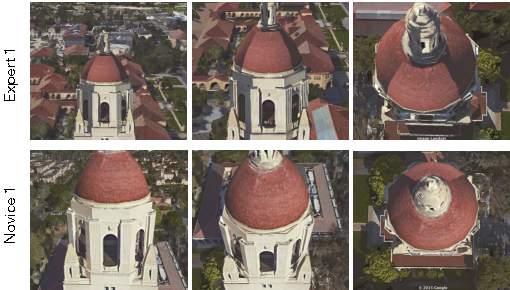
\includegraphics[width=4.0in]{images/2015_siggraph_asia/top-down-sequ.pdf}
\caption{
Novices and experts successfully designed shots with challenging camera motions using our tool.
The expert shot (top) is especially challenging to execute manually, since it requires smoothly changing the camera orientation to look down at Hoover Tower exactly as the quadrotor flies over it.
The novice shot (bottom) contains a similar camera motion.
}
\label{fig:ch2:expert_novice_comparison}
\end{figure}

\paragraph{Novices and Experts Successfully Designed Challenging Shots}
We asked the expert cinematographers to describe what elements were challenging about the shots they created, if they were to capture them with existing approaches for quadrotor cinematography.
Each expert identified camera motions in their shots that would either take many attempts, or would have to be modified to be less challenging.
We identified similar camera motions in the novice shots (see Figure \ref{fig:ch2:expert_novice_comparison}).
We summarize the similarities between novice and expert shots as follows,

\begin{itemize}

\item
Expert shot (c) required continuous re-orientation of the camera relative to the flight path, with the look-from trajectory in red arcing away from a fixed look-at point.
We found a similar arcing motion around a fixed look-at point in novice shots (g) and (h).
This camera motion is difficult to execute manually, because it requires continuously and precisely re-orienting the camera during flight.

\item
Expert shot (a) required flying straight towards a point over a long distance, which we also found in novice shot (f).
This camera motion is difficult to execute manually, since small initial errors in the direction of flight have to be corrected, leading to visual artifacts in the resulting video.

\item
Expert shot (a) required smoothly adjusting the rate of camera re-orientation, to end at a specific orientation at a specific time.
We found this camera motion in novice shot (a).
We show these two shots in Figure \ref{fig:ch2:expert_novice_comparison}.
This camera motion is especially difficult to execute manually.
The camera must translate towards a point while tilting down, so that the end of the tilting motion exactly coincides with being above the tower, all while approaching the tower in a straight line.
The expert that designed shot (a) remarked that executing such a shot manually would require approximately 20 attempts.

\end{itemize}

This finding suggests that users can successfully design compelling shots with challenging camera motions using our tool, regardless of their level of expertise with quadrotors.

\paragraph{Previewing Shots Visually was Useful}
Our exit survey asked participants to identify the most useful feature of our user interface, and rank the features in our user interface on a 5-point scale from \emph{not useful} to \emph{indispensable}.
Three of the four participants identified the ability to visually preview their shot as being the most useful, and all users rated this feature as a 4 or higher.
%Several participants asked about the accuracy of this preview.
Indeed, Figure \ref{fig:ch1:teaser_ch2} shows that our visual preview accurately estimates the appearance of recorded video footage.
This finding validates our approach of enabling users to design shots visually, and highlights the importance of ensuring physical feasibility during the design process.

\begin{figure}[t]
\centering
\includegraphics[width=4.0in]{images/2015_siggraph_asia/edit-infeasible.pdf}
\caption{
Participants were able to modify infeasible shots into feasible shots using the visual feedback we provide in our tool.
After his \nth{7} revision, Expert 1 found that his shot was infeasible (left).
He edited both the altitude and timing of 3 keyframes to create a feasible shot as his \nth{8} revision (right).
Horizontal red lines indicate physical limits of our quadrotor hardware.
}
\label{fig:ch2:feasibility_fix}
\end{figure}

\paragraph{Controlling the Timing of Shots was Useful}
All participants used the easing curves to refine the timing of their shots.
Participants used the easing curves to modify the pacing of their shots, and to fix feasibility violations.
In all shots, participants adjusted the default easing curve control points.
Of the eight shots created, six featured additional control points added by the participant.
This finding validates our approach of enabling users to precisely control the timing of their shots.

\paragraph{Visual Feasibility Feedback was Useful, Although Some Participants Would Have Preferred an Automatic Solution}
All of our participants responded to the visual feasibility feedback in our tool.
Users successfully modified their shots until they were within the physical limits of our hardware, as shown on the feasibility plots in our tool.
Figure \ref{fig:ch2:feasibility_fix} shows Expert 1 modifying both the altitude and timing of three keyframes to stay within the vertical speed limit of our quadrotor.
However, participants were divided in their opinions about our feasibility plots.
One participant rated it as the best part of the tool.
He described it as essential to creating shots at the physical limits of the hardware.
Another participant expressed difficulty knowing exactly how to tweak trajectories in response to the visual feedback.
This finding suggests that some users would prefer an automatic solution for fixing feasibility issues, while others like precise control over their shots.
We believe that developing an automatic solution to fix feasibility violations is an interesting direction for future work.

\begin{tcolorbox}[before skip=20pt, after skip=20pt, sharp corners]
\begin{center}
\textbf{In Chapter \ref{sec:ch3}, we will present an automatic algorithm for correcting feasibility violations.}
\end{center}
\end{tcolorbox}

\begin{figure}[t]
\centering
\includegraphics[width=4.0in]{images/2015_siggraph_asia/errors.pdf}
\caption{
Position and velocity error of our quadrotor for the longest (left) and shortest (right) shots.
The position error is less than 3.01m at all times, and the velocity error is less than 0.80m/s at all times.
Note that the horizontal scaling varies varies on the left and right subplots. 
}
\label{fig:ch2:errors}
\end{figure}

\paragraph{Accuracy}
To quantify how well our quadrotor camera system follows trajectories, we compared the intended trajectories created by our users, to the actual trajectories executed by our quadrotor (see Figure \ref{fig:ch2:errors}).
The average position error across all shots was 1.12m ($\sigma = 0.57$), and was never greater than 3.01m.
The average velocity error across all shots was 0.11m/s ($\sigma = 0.10$), and was never greater than 0.80m/s.
In general, our system is limited by the positioning and pointing accuracy of our quadrotor.
This limitation makes close-up shots particularly challenging, where small errors in position lead to more noticeable visual errors.
However, our participants responded positively when they saw the captured footage for the shots they created.
This finding suggests that the level of accuracy achievable with current-generation quadrotor hardware is sufficient to obtain a variety of compelling shots.

\paragraph{Concluding Remarks}
Overall, all participants were enthusiastic about using our system.
%In particular, they remarked on the usefulness of having a 3D camera view to visualize their shot.
%Indeed, Figure \ref{fig:teaser} shows that our visual preview accurately estimates the appearance of the recorded video footage.
Experts appreciated having a powerful tool to visually plan complex trajectories and execute repeatable takes (e.g. Expert 1 remarked \emph{``Normally I fly less ambitious paths to avoid making mistakes!''} and \emph{``I love how I can get the same shot, take after take, day after day!''}).
Novices were particularly enthusiastic about being able to capture high-quality video footage with quadrotors without having experience flying them (e.g., Novice 2 remarked, \emph{``I liked how it turned a `drone flying problem' into a `drawing a curve in space problem'. I don't know how to fly a drone and don't want to, but I find drawing in 3D very intuitive.'}').

\section{Conclusions}

We introduced a set of design principles for quadrotor shot planning tools.
Based on these principles, we built a tool for designing quadrotor camera shots.
Specifically, we added four components to current quadrotor mission planning tools: (1) visual shot design; (2) virtual preview; (3) precise timing control; and (4) visual feasibility feedback. 
Using our tool, both novices and expert users designed compelling shots that would be challenging to create otherwise.
We successfully and autonomously captured all shots with reasonable accuracy on a real quadrotor camera platform.

In the future, we believe quadrotors will enable many creative applications beyond the pre-scripted aerial cinematography shown in this paper.
Quadrotor cameras might soon be able to autonomously film a person skiing down a mountain, or a pack of wild animals hunting prey. 
By flying the same trajectory repeatedly, quadrotor cameras could also enable new kinds of highly dynamic time-lapse video footage.
Moving beyond the domain of cinematography, quadrotor cameras could help to reconstruct virtual 3D models of the physical world with unprecedented coverage and scale.

\section*{Acknowledgements}
We thank the anonymous reviewers for their valuable feedback;
Maxine Lim for her assistance in creating figures, and for designing our project website;
Jane E, James Hegarty, Wilmot Li, and Jerry Talton for their valuable feedback on early drafts of this paper;
Stephen Boyd for the helpful discussion about the optimization problem in Section 7;
Andrew Tridgell, Randy MacKay, and the \textsc{ArduPilot} team for their software support;
\textsc{3D Robotics} for their hardware support;
the professional cinematographers we interviewed, as well as our user study participants, for their time and valuable insights.
This work was supported in part by a NSERC Alexander Graham Bell Canada Graduate Scholarship.
Finally, we dedicate this paper in loving memory of our dear friend and valued collaborator, Floraine Berthouzoz.

%In the near future, we are incorporating a centimeter-accurate GPS into our quadrotor to further improve accuracy.
%We are also experimenting with approaches to algorithmically find feasible trajectories whenever the user creates an infeasible shot.

%More broadly speaking, we believe quadrotor cameras could enable many creative applications beyond the scripted aerial cinematography shown in this paper.
%Quadrotor cameras might soon be able to autonomously film a person skiing down a mountain, or a pack of wild animals hunting prey. 
%By flying the same trajectory repeatedly, quadrotor cameras could also enable new kinds of highly dynamic timelapse video footage.
%Moving beyond the domain of cinematography, quadrotor cameras could help reconstruct virtual 3D models of the physical world with unprecedented coverage and scale.


% \appendix

\section{Defining the Quadrotor Camera Manipulator Matrices}
\label{appendix:manipulator}

In this appendix, we define the quadrotor camera manipulator matrices, attempting to be as concise as possible.
We include a detailed derivation of these matrices in the supplementary material.

We begin by defining the layout of our degree-of-freedom vector $\mathbf{q}$, and our control vector $\mathbf{u}$, as follows,
%
\footnotesize
\begin{equation}
\mathbf{q} = 
\begin{bmatrix}
\mathbf{p} \\
\mathbf{e}_q \\
\mathbf{e}_g
\end{bmatrix}
%
~~~~
\mathbf{u} = 
\begin{bmatrix}
\mathbf{u}_q \\
\mathbf{u}_g
\end{bmatrix}
\end{equation}
\normalsize
%
where $\mathbf{p}$ is the position of the quadrotor's center of mass; $\mathbf{e}_q$ is the vector of Euler angles representing the quadrotor's orientation in the world frame; $\mathbf{e}_g$ is the vector of Euler angles representing the orientation of the gimbal in the body frame of the quadrotor; $\mathbf{u}_q$ is the thrust control we apply at the quadrotor propellors; and $\mathbf{u}_g$ is the torque control we apply at the gimbal.

We express the manipulator matrices for our quadrotor camera system as follows,
%
\footnotesize
\begin{equation}
\begin{aligned}
\mathbf{H}(\mathbf{q}) = &
\begin{bmatrix}
m\mathbf{I}_{3\times3} & \mathbf{0}_{3\times3} & \mathbf{0}_{3\times3} \\
\mathbf{0}_{3\times3}                          & \mathbf{I}_{q} \mathbf{R}_{\mathcal{Q},\mathcal{W}} \mathbf{A}_q & \mathbf{0}_{3\times3} \\
\mathbf{0}_{3\times3}                          & \mathbf{0}_{3\times3} & \mathbf{A}_{g}
\end{bmatrix} \\
%
\mathbf{C}(\mathbf{q},\dot{\mathbf{q}}) = &
\end{aligned} \notag
\end{equation}
%
\vspace{-10pt}
\begin{equation}
\begin{aligned}
\begin{bmatrix}
\mathbf{0}_{3\times3} & \mathbf{0}_{3\times3}  & \mathbf{0}_{3\times3} \\
\mathbf{0}_{3\times3} & \mathbf{I}_q \mathbf{R}_{\mathcal{Q},\mathcal{W}} \dot{\mathbf{A}}_q - \left(\mathbf{I}_q \mathbf{R}_{\mathcal{Q},\mathcal{W}} \mathbf{A}_q \dot{\mathbf{e}}_q \right)_{\times}\mathbf{R}_{\mathcal{Q},\mathcal{W}} \mathbf{A}_q & \mathbf{0}_{3\times3} \\
\mathbf{0}_{3\times3} & \mathbf{0}_{3\times3}  & \dot{\mathbf{A}}_g
\end{bmatrix}
\end{aligned} \notag
\end{equation}
%
\begin{equation}
\begin{aligned}
\mathbf{G}(\mathbf{q}) = &
\begin{bmatrix}
-\mathbf{f}_e \\
\mathbf{0}_{3\times1} \\
\mathbf{0}_{3\times1} \\
\end{bmatrix} \\
%
\mathbf{B}(\mathbf{q}) = &
\begin{bmatrix}
\mathbf{R}_{\mathcal{W},\mathcal{Q}} \mathbf{M}_{\mathbf{f}}    & \mathbf{0}_{3\times3} \\
\mathbf{M}_{\mathbf{\tau}}                                      & \mathbf{0}_{3\times3} \\
\mathbf{0}_{3\times4}                                           & \mathbf{I}_{3\times3} \\
\end{bmatrix} ~~~~~~~~~~~~~\text{}
\end{aligned}
\end{equation}
%
\normalsize
where $m$ is the mass of the quadrotor camera;
$\mathbf{I}_q$ is the inertia matrix of the quadrotor camera;
$\mathbf{R}_{\mathcal{W},\mathcal{Q}}$ is the rotation matrix that represents the quadrotor's orientation in the world frame (i.e., the rotation matrix that maps vectors from the body frame of the quadrotor into the world frame);
$\mathbf{R}_{\mathcal{Q},\mathcal{W}}$ is the rotation matrix that maps vectors from the world frame into the body frame of the quadrotor;
$\mathbf{A}_q$ is the matrix that relates the quadrotor's Euler angle time derivatives to its angular velocity in the world frame;
$\mathbf{A}_g$ is the matrix that relates the gimbal's Euler angle time derivatives to its angular velocity in the body frame of the quadrotor;
$\mathbf{f}_e$ is the external force;
$\mathbf{M}_{\mathbf{f}}$ is the matrix that maps the control input at each of the quadrotor's propellers into a net thrust force oriented along the quadrotor's local $\mathbf{y}$ axis;
$\mathbf{M}_{\mathbf{\tau}}$ is the matrix that maps the control input at each of the quadrotor's propellers into a net torque acting on the quadrotor in the body frame;
$\mathbf{0}_{p \times q}$ is the $p \times q$ zero matrix;
$\mathbf{I}_{k \times k}$ is the $k \times k$ identity matrix;
and the notation $\left( \mathbf{a} \right)_{\times}$ refers to the skew-symmetric matrix, computed as a function of the vector $\mathbf{a}$, such that $\left(\mathbf{a}\right)_{\times}\mathbf{b} = \mathbf{a}\times\mathbf{b}$ for all vectors $\mathbf{b}$.

Our expressions for the quadrotor camera manipulator matrices depend on the matrices, $\mathbf{M}_{\mathbf{f}}$ and $\mathbf{M}_{\mathbf{\tau}}$.
We define these matrices as follows, 
%
\footnotesize
\begin{equation}
\begin{aligned}
%
\mathbf{M}_{\mathbf{f}} = &
\begin{bmatrix}
0 & 0 & 0 & 0 \\
1 & 1 & 1 & 1 \\
0 & 0 & 0 & 0 \\
\end{bmatrix}\\
%
\mathbf{M}_{\mathbf{\tau}} = &
\begin{bmatrix}
 ds_\alpha & ds_\beta & -ds_\beta & -ds_\alpha \\
\gamma     & -\gamma  & \gamma    & -\gamma    \\
-dc_\alpha & dc_\beta & dc_\beta  & -dc_\alpha \\
\end{bmatrix}
%
\end{aligned}
\end{equation}
\normalsize
%%
where $d$, $\alpha$, $\beta$, and $\gamma$ are constants related to the physical design of a quadrotor:
$d$ is the distance from the quadrotor's center of mass to its propellers;
$\alpha$ is the angle in radians that the quadrotor's front propellers form with the quadrotor's positive $\mathbf{x}$ axis;
$\beta$ is the angle in radians that the quadrotor's rear propellers form with the quadrotor's negative $\mathbf{x}$ axis;
$\gamma$ is the magnitude of the in-plane torque generated by the quadrotor propeller producing 1 unit of upward thrust force;
$c_a=\cos a$ and $s_a=\sin a$.

Note that our expressions for the quadrotor camera manipulator matrices, in particular our expressions for $\mathbf{A}_q$ and $\mathbf{A}_g$, depend on our choice of Euler angle conventions.
See our derivation in the supplementary material for details.

%Our expressions for the quadrotor camera manipulator matrices also depend on our choice of Euler angle conventions.
%Throughout this paper, we adopt the following Euler angle conventions.
%Let $\mathbf{e} = [ \theta ~ \psi ~ \phi ]^T$ be a vector of Euler angles, and let $\omega$ be angular velocity in the non-rotating frame as these Euler angles change over time. We define the corresponding rotation matrix $\mathbf{R}$ in terms of the Euler angles $\theta$, $\psi$, and $\phi$ as follows,
%%
%\footnotesize
%\begin{equation}
%\begin{aligned}
%%
%\mathbf{R} & = \mathbf{R}_{\mathbf{y}}^{\psi} \mathbf{R}_{\mathbf{z}}^{\theta} \mathbf{R}_{\mathbf{x}}^{\phi} \\
%& = 
%\begin{bmatrix}
%c_\psi  & 0 & s_\psi \\
%0       & 1 & 0 \\
%-s_\psi & 0 & c_\psi \\
%\end{bmatrix}
%\begin{bmatrix}
%1 & 0        & 0 \\
%0 & c_\theta & -s_\theta \\
%0 & s_\theta & c_\theta \\
%\end{bmatrix}
%%
%\begin{bmatrix}
%c_\phi & -s_\phi & 0 \\
%s_\phi & c_\phi  & 0 \\
%0      & 0       & 1 \\
%\end{bmatrix}
%%
%\end{aligned}
%\end{equation}
%\normalsize
%%
%where $c_a=\cos a$ and $s_a=\sin a$.
%Finally, we define the matrix $\mathbf{A}$ that relates $\dot{\mathbf{e}}$ to $\omega$ according to the linear relationship $\mathbf{A} \dot{\mathbf{e}} = \omega$, and its time derivative $\dot{\mathbf{A}}$, as follows,
%%
%\footnotesize
%\begin{equation}
%\begin{aligned}
%%
%\mathbf{A} & =
%\begin{bmatrix}
%c_\psi  & 0 & s_\psi c_\theta \\
%0       & 1 & -s_\theta       \\
%-s_\psi & 0 & c_\psi c_\theta \\
%\end{bmatrix} \\
%%
%\dot{\mathbf{A}} & =
%\begin{bmatrix}
%-s_\psi \dot{\psi} & 0 & -s_\psi s_\theta \dot{\theta} + c_\psi c_\theta \dot{\psi} \\
%0                  & 0 & -c_\theta \dot{\theta} \\
%-c_\psi \dot{\psi} & 0 & -s_\psi c_\theta \dot{\psi} + s_\theta c_\psi \dot{\theta} \\
%\end{bmatrix}
%%
%\end{aligned}
%\end{equation}
%\normalsize
%%
%where $c_a=\cos a$ and $s_a=\sin a$.

%%% template.tex
%%%
%%% This LaTeX source document can be used as the basis for your technical
%%% paper or abstract.

%%% The parameter to the ``documentclass'' command is very important.
%%% - use ``e'' for content submitted for review.
%%% - use ``preprint'' for accepted content you are making available.
%%% - use ``tog'' for technical papers accepted to the TOG journal and
%%%   for presentation at the SIGGRAPH or SIGGRAPH Asia conference.
%%% - use ``conference'' for final content accepted to a sponsored event
%%%   (hint: If you don't know, you should use ``conference.'')

% \documentclass[tog]{acmsiggraph}

% \usepackage[numbered]{algorithm}
% \usepackage[noend]{algorithmic}
% \usepackage[super]{nth}

% %%% Make the ``BibTeX'' word pretty...

% \def\BibTeX{{\rm B\kern-.05em{\sc i\kern-.025em b}\kern-.08em
%     T\kern-.1667em\lower.7ex\hbox{E}\kern-.125emX}}

% %%% Used by the ``review'' variation; the online ID will be printed on 
% %%% every page of the content.

% \TOGonlineid{0214}

% %%% Used by the ``preprint'' variation.

% \TOGvolume{0}
% \TOGnumber{0}

% \title{An Interactive Tool for Designing Quadrotor Camera Shots\\Supplementary Material}

% \author{Niels Joubert\thanks{Niels Joubert and Mike Roberts contributed equally to this work.}\\Stanford University \and Mike Roberts$^{*}$\\Stanford University \and Anh Truong\\Stanford University \and Floraine Berthouzoz\\Adobe Research \and Pat Hanrahan\\Stanford University}
% \pdfauthor{Niels Joubert, Mike Roberts, Anh Truong, Floraine Berthouzoz, Pat Hanrahan}

% \floatstyle{boxed}
% \newfloat{Listing}{t}{ext}

% \renewcommand{\algorithmicrequire}{\small\textbf{Input:}}
% \renewcommand{\algorithmicensure}{\small\textbf{Output:}}

% \DeclareMathOperator*{\argmin}{arg\,min}
% \usepackage{amstext}

% \begin{document}

% \maketitle

%\begin{CRcatlist}
%  \CRcat{I.3.3}{Computer Graphics}{Three-Dimensional Graphics and Realism}{Display Algorithms}
%  \CRcat{I.3.7}{Computer Graphics}{Three-Dimensional Graphics and Realism}{Radiosity};
%\end{CRcatlist}

%\TOGlinkslist
%\copyrightspace

%\section{Specification Sheet for the \textsc{IRIS} Camera Control System by \textsc{Bot \& Dolly}}

%\begin{figure*}[t]
%  \centering
%  \includegraphics[width=7.0in]{images/iris}
%  \caption{
%Specification sheet for the \textsc{IRIS} camera control system developed by \textsc{Bot \& Dolly}. This brochure owned by Bot \& Dolly, reproduced here for education purposes to aid our related work discussion of systems comparable to ours.
%}
%  \label{figure:iris}
%\end{figure*}

%\textsc{Bot \& Dolly}, the company that developed the \textsc{IRIS} camera control system, is now defunct.
%The specification sheet for the \textsc{IRIS} camera control system is no longer available online.
%We include it in Figure \ref{figure:iris} in this document for completeness.

\subsection{Deriving the Quadrotor Camera Manipulator Matrices}
\label{sec:ch2:manipulator_detail}

In this subsection, we derive the manipulator matrices for our quadrotor camera model.
At a high level, our strategy will be to relate our quadrotor camera's degrees of freedom to our control inputs.

In the derivation that follows, we assume that our quadrotor and gimbal are \emph{kinematically coupled}~\cite{kondak:2013}, in the sense that moving the position of the quadrotor also moves the position of the gimbal. However, we assume that our quadrotor and gimbal are not \emph{dynamically coupled}~\cite{kondak:2013}, in the sense that torques acting on the gimbal do not induce reactive torques on the quadrotor.
These assumptions simplify the modeling of our system. Moreover, we feel they are justified, since in the cameras mounted on quadrotors tend to be very lightweight relative to the quadrotors themselves. For example, on our hardware platform, our camera and gimbal are roughly 25$\times$ lighter than our quadrotor.

\paragraph{Relating the Quadrotor's Position to the Control Inputs}

We assume that there are two forces acting on our quadrotor camera: (1) a \emph{thrust force} induced by the quadrotor's propellers; and (2) an \emph{external force} that models any other forces acting on the quadrotor, such as gravity, wind, and drag.
Based on this assumption, we use Newton's Second Law to relate the linear acceleration of the quadrotor in the world frame, $\ddot{\mathbf{p}}$, to the control input applied at each of the quadrotor's propellers, $\mathbf{u}_q$, as follows,
%
\begin{equation}
m \ddot{\mathbf{p}} = \mathbf{f}_e + \mathbf{R}_{\mathcal{W},\mathcal{Q}} \mathbf{M}_{\mathbf{f}} \mathbf{u}_q
\label{eqn:ch2:m_p_dot_dot}
\end{equation}
%
where $m$ is the mass of the quadrotor camera; $\mathbf{f}_e$ is the external force; $\mathbf{M}_{\mathbf{f}}$ is the matrix that maps the control input at each of the quadrotor's propellers into a net thrust force oriented along the quadrotor's local $\mathbf{y}$ axis; and $\mathbf{R}_{\mathcal{W},\mathcal{Q}}$ is the rotation matrix that represents the quadrotor's orientation in the world frame (i.e., the rotation matrix that maps vectors from the body frame of the quadrotor into the world frame).
We define $\mathbf{M}_{\mathbf{f}}$ as follows, 
%
\begin{equation}
\begin{aligned}
%
\mathbf{M}_{\mathbf{f}} =
\begin{bmatrix}
0 & 0 & 0 & 0 \\
1 & 1 & 1 & 1 \\
0 & 0 & 0 & 0 \\
\end{bmatrix}
%
\end{aligned}
\end{equation}

\paragraph{Relating the Quadrotor's Angular Acceleration and Angular Velocity to the Control Inputs}

We use Euler's Second Law to relate the angular acceleration and angular velocity of the quadrotor in the body frame, $\dot{\mathbf{\omega}}_q$ and $\mathbf{\omega}_q$ respectively, to the control input applied at each of the quadrotor's propellers, $\mathbf{u}_q$, as follows,
%
\begin{equation}
\mathbf{I}_{q} \dot{\mathbf{\omega}}_q + \mathbf{\omega}_q \times \mathbf{I}_q \mathbf{\omega}_q = \mathbf{M}_{\mathbf{\tau}} \mathbf{u}_q
\label{eqn:ch2:M_t_u_q_short}
\end{equation}
%
where $\mathbf{I}_{q}$ is the inertia matrix of the quadrotor camera; and $\mathbf{M}_{\mathbf{\tau}}$ is the matrix that maps the control input at each of the quadrotor's propellers into a net torque acting on the quadrotor in the body frame.
We define $\mathbf{M}_{\mathbf{\tau}}$ as follows, 
%
\begin{equation}
\begin{aligned}
%
\mathbf{M}_{\mathbf{\tau}} =
\begin{bmatrix}
 ds_\alpha & ds_\beta & -ds_\beta & -ds_\alpha \\
\gamma     & -\gamma  & \gamma    & -\gamma    \\
-dc_\alpha & dc_\beta & dc_\beta  & -dc_\alpha \\
\end{bmatrix}
%
\end{aligned}
\end{equation}
%
where $d$, $\alpha$, $\beta$, and $\gamma$ are constants related to the physical design of a quadrotor:
$d$ is the distance from the quadrotor's center of mass to it's propellers;
$\alpha$ is the angle in radians that the quadrotor's front propellers form with the quadrotor's positive $\mathbf{x}$ axis;
$\beta$ is the angle in radians that the quadrotor's rear propellers form with the quadrotor's negative $\mathbf{x}$ axis;
$\gamma$ is the magnitude of the in-plane torque generated by the quadrotor propeller producing 1 unit of upward thrust force;
$c_a=\cos a$ and $s_a=\sin a$.
Our definition for $\mathbf{M}_{\mathbf{\tau}}$ assumes: (1) the quadrotor's propellers are co-planar with its center of mass; and (2) a constant relationship between the magnitude of the in-plane torque generated by the quadrotor propeller, and the magnitude of the upward thrust force generated by the propeller. 

\paragraph{Relating the Gimbal's Angular Acceleration to the Control Inputs}
We assume that our 3 degree-of-freedom gimbal is fully actuated, and has very large actuator limits. Since fully actuated systems are \emph{feedback equivalent}~\cite{tedrake:2016} to double integrator systems, and we assume that our gimbal has very large actuator limits, we model the gimbal as a double integrator for simplicity. We relate the angular acceleration of the gimbal in the body frame of the quadrotor, $\dot{\mathbf{\omega}}_g$ to the \emph{feedback linearized}~\cite{tedrake:2016} control input applied at the gimbal, $\mathbf{u}_g$, as follows,
%
\begin{equation}
\dot{\mathbf{\omega}}_g = \mathbf{u}_g
\label{eqn:ch2:u_g_short}
\end{equation}
%

\paragraph{Relating Euler Angle Time Derivatives to Angular Velocity and Angular Acceleration}

At this point, we have related the angular velocities and accelerations of our system to our control inputs.
However, to derive the complete equations of motion for our system, we need to relate the Euler angle time derivatives of our system to our control inputs.
To do this, we must relate Euler angle time derivatives to angular velocities and angular accelerations.

Let $\mathbf{e} = [ \theta ~ \psi ~ \phi ]^T$ be a vector of our Euler angles.
Let us define the rotation matrix $\mathbf{R}$ in terms of the Euler angles $\theta$, $\psi$, and $\phi$ as follows,
%
\begin{equation}
\begin{aligned}
%
\mathbf{R} & = \mathbf{R}_{\mathbf{y}}^{\psi} \mathbf{R}_{\mathbf{z}}^{\theta} \mathbf{R}_{\mathbf{x}}^{\phi} \\
& = 
\begin{bmatrix}
c_\psi  & 0 & s_\psi \\
0       & 1 & 0 \\
-s_\psi & 0 & c_\psi \\
\end{bmatrix}
\begin{bmatrix}
1 & 0        & 0 \\
0 & c_\theta & -s_\theta \\
0 & s_\theta & c_\theta \\
\end{bmatrix}
%
\begin{bmatrix}
c_\phi & -s_\phi & 0 \\
s_\phi & c_\phi  & 0 \\
0      & 0       & 1 \\
\end{bmatrix}
%
%
\end{aligned}
\end{equation}
%
where $c_a=\cos(a)$ and $s_a=\sin(a)$.

We can straightforwardly compute the time derivative of this expression to get an (admittedly unpleasant) expression for $\dot{\mathbf{R}}$ in terms of our Euler angles and their time derivatives.
We omit this step for brevity.

We make the observation that $\dot{\mathbf{R}} = (\mathbf{\omega})_{\times} \mathbf{R}$, where $\mathbf{\omega}$ is the angular velocity of a rotating body in the non-rotating frame; and the notation $\left( \mathbf{a} \right)_{\times}$ refers to the skew-symmetric matrix, computed as a function of the vector $\mathbf{a}$, such that $\left(\mathbf{a}\right)_{\times}\mathbf{b} = \mathbf{a}\times\mathbf{b}$ for all vectors $\mathbf{b}$. 

From the above expression, we immediately get $\dot{\mathbf{R}} \mathbf{R}^{T} = (\mathbf{\omega})_{\times}$.
We observe that the entries of $\dot{\mathbf{R}} \mathbf{R}^{T}$ are linear in  $\dot\psi$, $\dot\theta$, and $\dot\phi$.
Therefore, there is a matrix $\mathbf{A}$ that relates $\dot{\mathbf{e}}$ to $\omega$ as follows,
%
\begin{equation}
\mathbf{A} \dot{\mathbf{e}} = \mathbf{\omega}
\label{eqn:ch2:w}
\end{equation}
%
We can take the time derivative of both sides of this expression using the product rule to get the following expression,
%
\begin{equation}
\dot{\mathbf{A}} \dot{\mathbf{e}} + \mathbf{A} \ddot{\mathbf{e}} = \dot{\mathbf{\omega}}
\label{eqn:ch2:w_dot}
\end{equation}
%
We define the matrix $\mathbf{A}$ that relates $\dot{\mathbf{e}}$ to $\omega$ according to the linear relationship $\mathbf{A} \dot{\mathbf{e}} = \omega$, and its time derivative $\dot{\mathbf{A}}$, as follows,
%
\begin{equation}
\begin{aligned}
%
\mathbf{A} & =
\begin{bmatrix}
c_\psi  & 0 & s_\psi c_\theta \\
0       & 1 & -s_\theta       \\
-s_\psi & 0 & c_\psi c_\theta \\
\end{bmatrix} \\
%
\dot{\mathbf{A}} & =
\begin{bmatrix}
-s_\psi \dot{\psi} & 0 & -s_\psi s_\theta \dot{\theta} + c_\psi c_\theta \dot{\psi} \\
0                  & 0 & -c_\theta \dot{\theta} \\
-c_\psi \dot{\psi} & 0 & -s_\psi c_\theta \dot{\psi} + s_\theta c_\psi \dot{\theta} \\
\end{bmatrix}
%
\end{aligned}
\end{equation}
%
where $c_a=\cos a$ and $s_a=\sin a$.

\paragraph{Relating the Quadrotor's Orientation to the Control Inputs}

We can rotate equations~(\ref{eqn:ch2:w}) and (\ref{eqn:ch2:w_dot}) into the body frame of the quadrotor, and substitute them into equation~(\ref{eqn:ch2:M_t_u_q_short}), to get the following expression for the quadrotor's rotational dynamics,
%
\begin{equation}
\begin{aligned}
\mathbf{I}_{q} ( \mathbf{R}_{\mathcal{Q},\mathcal{W}} \dot{\mathbf{A}}_q \dot{\mathbf{e}}_q + \mathbf{R}_{\mathcal{Q},\mathcal{W}} \mathbf{A}_q \ddot{\mathbf{e}}_q ) + \mathbf{R}_{\mathcal{Q},\mathcal{W}} \mathbf{A}_q \dot{\mathbf{e}}_q \times \mathbf{I}_q \mathbf{R}_{\mathcal{Q},\mathcal{W}} \mathbf{A}_q \dot{\mathbf{e}}_q
=
\mathbf{M}_{\mathbf{\tau}} \mathbf{u}_q
\end{aligned}
\label{eqn:ch2:M_t_u_q_long}
\end{equation}
%
where
$\mathbf{e}_q$ is the vector of Euler angles representing the quadrotor's orientation in the world frame; 
$\mathbf{R}_{\mathcal{Q},\mathcal{W}}$ is the rotation matrix that maps vectors from the world frame into the body frame of the quadrotor;
and $\mathbf{A}_q$ is the matrix that relates the quadrotor's Euler angle time derivatives to its angular velocity in the world frame.

\paragraph{Relating the Gimbal's Orientation to the Control Inputs}

Similarly to our approach in the previous subsection, we can substitute equation~(\ref{eqn:ch2:w_dot}) into equation~(\ref{eqn:ch2:u_g_short}) to get the following expression for the gimbal's rotational dynamics,       
%
\begin{equation}
\dot{\mathbf{A}}_g \dot{\mathbf{e}}_g + \mathbf{A}_g \ddot{\mathbf{e}}_g = \mathbf{u}_g
\label{eqn:ch2:u_g_long}
\end{equation}
%
where
$\mathbf{e}_g$ is the vector of Euler angles representing the orientation of the gimbal in the body frame of the quadrotor;
and $\mathbf{A}_g$ is the matrix that relates the gimbal's Euler angle time derivatives to its angular velocity in the body frame of the quadrotor.

\paragraph{Defining the Manipulator Matrices}
We define the layout of our degree-of-freedom vector $\mathbf{q}$, and our control vector $\mathbf{u}$, as follows,
%
\begin{equation}
\mathbf{q} = 
\begin{bmatrix}
\mathbf{p} \\
\mathbf{e}_q \\
\mathbf{e}_g
\end{bmatrix}
%
~~~~
\mathbf{u} = 
\begin{bmatrix}
\mathbf{u}_q \\
\mathbf{u}_g
\end{bmatrix}
\end{equation}
%
Based on this layout, we can express equations~(\ref{eqn:ch2:m_p_dot_dot}), (\ref{eqn:ch2:M_t_u_q_long}), and (\ref{eqn:ch2:u_g_long}) in manipulator form.
In doing so, we get the following expressions for our quadrotor camera manipulator matrices,
%
\begin{equation}
\begin{aligned}
\mathbf{H}(\mathbf{q}) = &
\begin{bmatrix}
m\mathbf{I}_{3\times3} & \mathbf{0}_{3\times3} & \mathbf{0}_{3\times3} \\
\mathbf{0}_{3\times3}                          & \mathbf{I}_{q} \mathbf{R}_{\mathcal{Q},\mathcal{W}} \mathbf{A}_q & \mathbf{0}_{3\times3} \\
\mathbf{0}_{3\times3}                          & \mathbf{0}_{3\times3} & \mathbf{A}_{g}
\end{bmatrix} \\
%
\mathbf{C}(\mathbf{q},\dot{\mathbf{q}}) = &
\begin{bmatrix}
\mathbf{0}_{3\times3} & \mathbf{0}_{3\times3}  & \mathbf{0}_{3\times3} \\
\mathbf{0}_{3\times3} & \mathbf{I}_q \mathbf{R}_{\mathcal{Q},\mathcal{W}} \dot{\mathbf{A}}_q - \left(\mathbf{I}_q \mathbf{R}_{\mathcal{Q},\mathcal{W}} \mathbf{A}_q \dot{\mathbf{e}}_q \right)_{\times}\mathbf{R}_{\mathcal{Q},\mathcal{W}} \mathbf{A}_q & \mathbf{0}_{3\times3} \\
\mathbf{0}_{3\times3} & \mathbf{0}_{3\times3}  & \dot{\mathbf{A}}_g
\end{bmatrix} \\
%
\mathbf{G}(\mathbf{q}) = &
\begin{bmatrix}
-\mathbf{f}_e \\
\mathbf{0}_{3\times1} \\
\mathbf{0}_{3\times1} \\
\end{bmatrix} \\
%
\mathbf{B}(\mathbf{q}) = &
\begin{bmatrix}
\mathbf{R}_{\mathcal{W},\mathcal{Q}} \mathbf{M}_{\mathbf{f}}  & \mathbf{0}_{3\times3} \\
\mathbf{M}_{\mathbf{\tau}}                                    & \mathbf{0}_{3\times3} \\
\mathbf{0}_{3\times4}                                         & \mathbf{I}_{3\times3} \\
\end{bmatrix}
\end{aligned}
\end{equation}
%
where $\mathbf{0}_{p \times q}$ is the $p \times q$ zero matrix;
and $\mathbf{I}_{k \times k}$ is the $k \times k$ identity matrix.
In our definition for the manipulator matrices above, we assume that $\mathbf{f}_e$ can depend on $\mathbf{q}$, but cannot depend on $\dot{\mathbf{q}}$.
We make this assumption for simplicity, although it could be relaxed by making minor modifications to $\mathbf{C}$ and $\mathbf{G}$ above.

\begin{figure*}[t]
\centering
\includegraphics[width=6.0in]{images/2015_siggraph_asia_supplementary/method_comparison}
\caption{
Comparison of the quadrotor control signals resulting from different keyframe interpolation methods.
We construct a simple synthetic traejectory (a). We use the control signals required for a  quadrotor to follow the synthetic trajectory as ground truth (b).
We sample the synthetic trajectory with 15 evenly spaced keyframes, and we construct an interpolated trajectory from these keyframes using different interpolation methods.
We plot the control signals produced by each interpolation method. We require that the control signals be continuous, and we prefer control signals that are as close as possible to the ground truth. We show the middle of these control signal plots to highlight their periodic behavior without boundary artifacts.
For each interpolation method, we show the control signal for the front right propeller, and we indicate the control signal value at each keyframe with a blue dot.
\nth{3} degree Catmull Rom Splines are $C^1$ continuous, and therefore produce discontinuous control signals (c).
Natural Cubic Splines are $C^2$ continuous, and therefore also produce discontinuous control signals (d).
\nth{9} degree Catmull Rom Splines are $C^4$ continuous, so they produce continuous control signals, but with large periodic excursions (e).
Our method is $C^4$ continuous and produces control signals with minimal excursions (f). 
}
\label{fig:ch2:method_comparison}
\end{figure*}

\begin{figure*}[t!]
\centering
\includegraphics[width=6.0in]{images/2015_siggraph_asia_supplementary/parameter_comparison}
\caption{
Comparison of the quadrotor control signals resulting from different variations of our method when interpolating the synthetic trajectory described in Figure~\ref{fig:ch2:method_comparison}.
We show the middle of these control signal plots to highlight their periodic behavior without boundary artifacts.
For each variation of our method, we show the control signal for the front right propeller, and we indicate the control signal value at each keyframe with a blue dot. Note that the vertical scaling varies in each subplot, and is different from the vertical scaling in Figure~\ref{fig:ch2:method_comparison}.
Minimizing the \nth{4} derivative of \nth{7} degree polynomials (also shown, with different vertical scaling, in Figure~\ref{fig:ch2:method_comparison}f) is the simplest variation of our method that produces smooth and reasonably bounded control signals.
Note that  $C^4$ continuous position trajectories are only guaranteed to produce $C^0$ continuous control signals for quadrotors, which is why some of the control signals in this figure are jagged.
}
\label{fig:ch2:parameter_comparison}
\end{figure*}

\subsection{Empirical Justification for Minimizing the \nth{4} Derivative of \nth{7} Degree Polynomials}
\label{sec:ch2:derivative_experiment}

In this subsection, we evaluate alternative polynomial representations for quadrotor camera paths.
We find that minimizing the \nth{4} derivative of \nth{7} degree piecewise polynomials produces the smoothest and most reasonably bounded control signals for quadrotors (see Figures~\ref{fig:ch2:method_comparison} and \ref{fig:ch2:parameter_comparison} in this document).

When evaluating alternative polynomial representations, we chose to limit our experiments to odd degree (i.e., even order) polynomials, since these tend to produce smoother curves than even degree (i.e., odd order) polynomials~\cite{goshtasby:1990}.


\subsection{Proof that B is Always Full Column Rank}
\label{sec:ch2:rank}

To prove that the matrix $\mathbf{B}$ is full column rank, consider the following matrix,
%
\begin{equation}
\mathbf{M} = 
\begin{bmatrix}
\mathbf{R}_{\mathcal{W},\mathcal{Q}} \mathbf{M}_{\mathbf{f}} \\
\mathbf{M}_{\mathbf{\tau}}                                   \\
\end{bmatrix}
\end{equation}
%
It will suffice to show that $\mathrm{rank}(\mathbf{M})=4$.
We assume without loss of generality that $0 < \alpha,\beta < \frac{\pi}{2}$ and that $d,\gamma > 0$.
We can clearly see that $\mathrm{rank}(\mathbf{M}_{\mathbf{\tau}})=3$.

Suppose for the sake of contradiction that $\mathrm{rank}(\mathbf{M})=3$.
Then we must be able to represent any row of $\mathbf{R}_{\mathcal{W},\mathcal{Q}} \mathbf{M}_{\mathbf{f}}$ as a linear combination of the rows of $\mathbf{M}_{\mathbf{\tau}}$.
Let the row $\mathbf{r} =[r ~ r ~ r ~ r]$ be one such row of $\mathbf{R}_{\mathcal{W},\mathcal{Q}} \mathbf{M}_{\mathbf{f}}$.
Representing $\mathbf{r}$ as a linear combination of the rows in $\mathbf{M}_{\mathbf{\tau}}$, we get the following system of equations,
%
\begin{equation}
\begin{aligned}
r & = ~   i ds_{\alpha} & + & ~ j \gamma & - & ~ k dc_{\alpha} \\
r & = ~   i ds_{\beta}  & - & ~ j \gamma & + & ~ k dc_{\beta}  \\
r & = ~ - i ds_{\beta}  & + & ~ j \gamma & + & ~ k dc_{\beta}  \\
r & = ~ - i ds_{\alpha} & - & ~ j \gamma & - & ~ k dc_{\alpha}
\end{aligned}
\end{equation}
%
for some $i,j,k$.
Equating the first and last of these equations above, we get $i ds_{\alpha} = - j \gamma $.
Equating the middle two of these equations above, we get $i ds_{\beta} =  j \gamma $.
Substituting these two new expressions into the first two equations above, we get $c_{\alpha} = - c_{\beta}$.
However, this is only possible if $\alpha$ or $\beta$ is outside the range $(0,\frac{\pi}{2})$.
Since we had previously assumed that $\alpha$ and $\beta$ are both inside the range $(0,\frac{\pi}{2})$, we have arrived at a contradiction.
This completes our proof.

% \section*{Acknowledgements}

% We thank Tao Du for catching and correcting an error in equation (9) in this document.

% \bibliographystyle{acmsiggraph}
% \bibliography{00_main}

% \end{document}




\chapter{Generating Dynamically Feasible Trajectories for Quadrotor Cameras}

\section{Teaser}

 % \teaser{
 %   \includegraphics[width=7.0in]{images/teaser.pdf}

 %   \caption{
 %   (Left) Our interactive tool for designing quadrotor camera shots.
 %   In our tool, users specify camera pose keyframes in a virtual environment using a 3D scene view (a) and a 2D map view (b).
 %   Our tool synthesizes a camera trajectory that obeys the physical equations of motion for quadrotors, and interpolates between the user-specified keyframes.
 %   Users can preview the resulting shot in the virtual environment, using the playback buttons and scrubber interface to navigate through the shot (c).
 %   Users can also control the precise timing of the shot by editing easing curves (d).
 %   Users can set the virtual camera's field of view to match their real-world camera (e).
 %   Our tool provides the user with visual feedback about the physical feasibility of the resulting trajectory, notifying the user if her intended trajectory violates the physical limits of her quadrotor hardware (f).
 %   Once the user is satisfied with her shot, she presses the Start Capture button (g).
 %   (Right) Our tool commands a quadrotor camera to execute the resulting trajectory fully autonomously, capturing real video footage that is faithful to the virtual preview.
 %   We show frames from our real-world video output, with corresponding frames from the virtual preview shown as small insets (h).
 %   }
 %   \label{fig:teaser}
 % }

\begin{figure*}[th!]
  \centering
  \includegraphics[width=5.5in]{images/2015_siggraph_asia/teaser.pdf}
  \caption{
(Left) Our interactive tool for designing quadrotor camera shots.
In our tool, users specify camera pose keyframes in a virtual environment using a 3D scene view (a) and a 2D map view (b).
Our tool synthesizes a camera trajectory that obeys the physical equations of motion for quadrotors, and interpolates between the user-specified keyframes.
Users can preview the resulting shot in the virtual environment, using the playback buttons and scrubber interface to navigate through the shot (c).
Users can also control the precise timing of the shot by editing easing curves (d).
Users can set the virtual camera's field of view to match their real-world camera (e).
Our tool provides the user with visual feedback about the physical feasibility of the resulting trajectory, notifying the user if her intended trajectory violates the physical limits of her quadrotor hardware (f).
Once the user is satisfied with her shot, she presses the Start Capture button (g).
(Right) Our tool commands a quadrotor camera to execute the resulting trajectory fully autonomously, capturing real video footage that is faithful to the virtual preview.
We show frames from our real-world video output, with corresponding frames from the virtual preview shown as small insets (h).
  }
  \label{fig:teaser}
\end{figure*}

% \begin{abstract}

% Cameras attached to small quadrotor aircraft are rapidly becoming a ubiquitous tool for cinematographers, enabling dynamic camera movements through 3D environments.
% Currently, professionals use these cameras by flying quadrotors manually, a process which requires much skill and dexterity. 
% In this paper, we investigate the needs of quadrotor cinematographers, and build a tool to support video capture using quadrotor-based camera systems.
% We begin by conducting semi-structured interviews with professional photographers and videographers, from which we extract a set of design principles.
% We present a tool based on these principles for designing and autonomously executing quadrotor-based camera shots.
% Our tool enables users to: (1) specify shots visually using keyframes; (2) preview the resulting shots in a virtual environment; (3) precisely control the timing of shots using easing curves; and (4) capture the resulting shots in the real world with a single button click using commercially available quadrotors.
% We evaluate our tool in a user study with novice and expert cinematographers.
% We show that our tool makes it possible for novices and experts to design compelling and challenging shots, and capture them fully autonomously.

% \end{abstract}

\section{Abstract}

Cameras attached to small quadrotor aircraft are rapidly becoming a ubiquitous tool for cinematographers, enabling dynamic camera movements through 3D environments.
Currently, professionals use these cameras by flying quadrotors manually, a process which requires much skill and dexterity. 
In this paper, we investigate the needs of quadrotor cinematographers, and build a tool to support video capture using quadrotor-based camera systems.
We begin by conducting semi-structured interviews with professional photographers and videographers, from which we extract a set of design principles.
We present a tool based on these principles for designing and autonomously executing quadrotor-based camera shots.
Our tool enables users to: (1) specify shots visually using keyframes; (2) preview the resulting shots in a virtual environment; (3) precisely control the timing of shots using easing curves; and (4) capture the resulting shots in the real world with a single button click using commercially available quadrotors.
We evaluate our tool in a user study with novice and expert cinematographers.
We show that our tool makes it possible for novices and experts to design compelling and challenging shots, and capture them fully autonomously.

% \section{Introduction}

\label{sec:ch3}

When designing trajectories for quadrotor cameras, it is important that the  trajectories respect the dynamics and physical limits of quadrotor hardware.
We refer to such trajectories as being \emph{feasible}.
If a quadrotor attempts to execute an \emph{infeasible}  trajectory, 
the quadrotor can deviate significantly from the intended trajectory, or even crash.
In addition, the virtual camera previews shown in existing shot planning tools will be visually accurate only if a shot is feasible.

Despite the importance of reasoning about feasibility in the design process, existing tools do not provide automatic methods for guaranteeing feasibility.
At best, existing tools \emph{notify} users when their trajectories are infeasible, but offer no guidance on how to \emph{modify} these trajectories to make them feasible.
It can be challenging for users to manually edit their trajectories to be feasible,  while preserving their original artistic intent. Indeed, requiring users to perform this type of manual editing can be quite burdensome, even for experienced users, since it requires users to reason explicitly about the non-linear quadrotor dynamics.

In this paper, we introduce a fast and user-friendly algorithm for generating feasible quadrotor camera trajectories.
Our algorithm takes as input an infeasible trajectory designed by a user, and produces as output a feasible trajectory that is as similar as possible to the user's input.
By design, our algorithm does not change the spatial layout or  visual contents of the input trajectory.
Instead, our algorithm guarantees the feasibility of the output trajectory by \emph{re-timing} the input trajectory, perturbing its timing as little as possible while remaining within velocity and control force limits.
Using our algorithm, a shot designer can modify a shot to be feasible with a single button click, completely preserving the visual contents of her shot.
We demonstrate the behavior of our algorithm in Figure \ref{fig:ch1:teaser_ch3}.

Our choice to perturb the timing of a shot, while leaving the spatial layout and visual contents of the shot intact, leads to a well-behaved non-convex optimization problem that can be solved at interactive rates.
To formulate our problem, we begin by analyzing the non-linear dynamics of a rigid body quadrotor along a fixed path.
Based on this analysis, we make two important observations that motivate our approach.
First, we observe that the full state of the quadrotor, as well as all necessary control forces, are fully determined by the \emph{progress curve} of the quadrotor along the path.
Second, we observe that all sufficiently smooth progress curves satisfy the non-linear quadrotor dynamics.

Based on the two observations above, we explicitly optimize for the progress curve (and hence, the re-timing of the input trajectory)\ that best agrees with the user's original input, subject to velocity and control force limits.
%We measure the agreement between the speed profile we're solving for, and the user's input trajectory, with a convex quadratic objective. We express velocity and control force limits as non-convex inequality constraints on the speed profile we're solving for.
Compared to existing trajectory optimization approaches, our approach has three major advantages. First, our approach requires fewer decision variables.
Second, our approach avoids slow-to-converge non-linear equality constraints that encode the system dynamics.
Third, our approach always provides an iterative solver with a well-defined search direction to fall back on, when attempting to satisfy inequality constraints.
%since slowing down the speed profile (i.e., driving the speed profile closer to zero, thereby forcing the quadrotor to execute the trajectory slower) always results in a closer-to-feasible trajectory.
Together, these advantages enable an off-the-shelf solver to make very rapid progress towards an optimal solution, ultimately leading to the interactive performance of our algorithm.

We demonstrate the utility of our algorithm by implementing it in \textsc{Horus}, the tool for designing quadrotor camera shots introduced in Chapter~\ref{sec:ch2}, where we achieve interactive performance across a wide range of camera trajectories.
We also apply our algorithm to a dataset of 8 infeasible camera trajectories, designed by 2 novice and 2 expert quadrotor cinematographers.
In all our experiments, our algorithm successfully solves for optimal trajectories in less than 2 seconds, and is between 25$\times$ and 45$\times$ faster than a spacetime constraints approach implemented using a commercially available solver.
As we scale to more finely discretized trajectories, this performance gap widens, with our algorithm outperforming spacetime constraints by between 90$\times$ and 180$\times$.
Our algorithm is also more accurate than spacetime constraints, predicting the results of \nth{5} order accurate rigid body physics simulations with lower average error.
Finally, we fly 5 feasible trajectories generated by our algorithm on a real quadrotor camera, producing video footage that is faithful to \textsc{Google Earth} shot previews, even when the trajectories are at the quadrotor's physical limits.

\section{Related Work}

\paragraph{Design Tools for Quadrotor Camera Trajectories}

Several tools exist for designing quadrotor camera trajectories.
These tools allow users to place waypoints on a 2D map~\cite{apm:2015,dji:2015} or in a 3D virtual environment~\cite{meier:2012,joubert:2015,gebhardt:2016}.
Other tools allow users to interactively control the speed and orientation of a quadrotor camera as it flies along a pre-determined trajectory~\cite{3drobotics:2015,dji:2015a,joubert:2015}. 
However, most existing tools do not reason explicitly about the quadrotor dynamics, and therefore do not offer any assurance that the user's intended shot is feasible.

%\cite{3drobotics:2015,apm:2015,dji:2015a,dji:2015,meier:2012}

The shot planning tool introduced in Chapter~\ref{sec:ch2} computes velocities and control forces along a user-specified trajectory, notifying the user if her shot is infeasible. However, this tool offers no guidance on how to modify the shot to make it feasible.
The tool introduced by Gebhardt et al.~\shortcite{gebhardt:2016} optimizes quadrotor camera trajectories subject to velocity and control force limits, and is therefore capable of generating feasible trajectories.
However, this tool uses an approximate linear model of the quadrotor dynamics, which is only accurate for conservative trajectories.
In contrast, our algorithm reasons explicitly about the non-linear quadrotor dynamics, and is applicable to aggressive trajectories that are at a quadrotor's physical limits.

Using existing tools, a simple strategy for capturing an infeasible shot would be to uniformly time-stretch the shot until it is feasible, and then time-warp the resulting video footage back to the original timing.
However, this strategy is only applicable in completely static scenes.
For example, if a person is walking through the scene, then their walking motion will be time-warped, which may be visually jarring.

%However, this tool optimizes the spatial layout of the user's intended trajectory, not the timing, and is therefore not guaranteed to find a dynamically feasible solution.
%Moreover, this tool uses an approximate linear model of the quadrotor dynamics, which is only accurate for conservative trajectories.
%In contrast, our algorithm is guaranteed to find a dynamically feasible re-timing of the user's intended trajectory, without disturbing its visual contents or spatial layout.
%Moreover, our algorithm reasons explicitly about the non-linear quadrotor dynamics, and is applicable to aggressive trajectories that are at a quadrotor's physical limits.

\paragraph{Trajectory Optimization Methods for Quadrotors}

%These spline-based methods take advantage of the fact that all $C^4$ continuous trajectories satisfy the non-linear quadrotors dynamics.
%However, the trajectories generated by these methods are not guaranteed to remain within velocity and control force limits.

The most common approach for optimizing quadrotor trajectories is to generate $C^4$ continuous splines that minimize some kind of bending energy~\cite{mellinger:2011,bry:2015,deits:2015,joubert:2015}.
These spline-based trajectories can be adapted to remain within velocity and control force limits by optimizing the time allocated to each spline segment~\cite{mellinger:2011,bry:2015}.
However, this approach can result in overly conservative trajectories in cases where a long spline segment is only briefly infeasible.
In contrast, our algorithm optimally re-times trajectories at the level of individual samples along a path, rather than at the level of spline segments, resulting in trajectories that more closely match a user's intended timing.

More general non-convex optimization methods have been applied to generate feasible quadrotor trajectories.
Similar to our approach in this paper, some of these methods explicitly optimize a progress curve~\cite{cowling:2007,bouktir:2008,vanloock:2013}.
However, these methods focus on finding the fastest or most fuel-efficient trajectory that reaches a goal, and typically also optimize the spatial layout of the trajectory.
In contrast, we treat the spatial layout of the trajectory as fixed, and we focus on finding the progress curve that most closely matches a user's input.

\paragraph{Trajectory Optimization Methods in Computer Graphics and Robotics}

The problem of optimizing trajectories for dynamical systems has been studied extensively in the computer  graphics literature~\cite{geijtenbeek:2012}, and in the robotics literature~\cite{betts:1998}.
A common approach in both communities is to discretize a trajectory into a sequence of system states, and encode the system dynamics into an optimization problem as a set of equality constraints.
%Optimal trajectories can then be found by minimizing an objective (e.g., control effort, or disagreement with a reference trajectory) subject to the equality constraints.
This approach is known as \emph{spacetime constraints} in the computer graphics community~\cite{witkins:1988}, and \emph{direct collocation} in the robotics community~\cite{betts:1998}.
We refer the reader to Fang and Pollard~\shortcite{fang:2003} and Safonova et al.~\shortcite{safonova:2004} for a detailed overview of spacetime constraints approaches in computer graphics.
A well-known limitation of spacetime constraints is that it slow to converge for highly non-linear systems, such as quadrotors.
In contrast, our approach avoids this slow convergence behavior, due to our analysis of the non-linear quadrotor dynamics along a fixed path.

Trajectory optimization problems along a fixed path have been studied in the computer graphics literature~\cite{mccann:2006}, and even more extensively in the robotics literature~\cite{shin:1985,slotine:1989,dahl:1990,verscheure:2009,lipp:2014}.
Existing methods require a path through a system's full \emph{configuration space} as input, and optimize the speed of the system along this path.
However, these methods are not applicable to quadrotors.
This is because a quadrotor's orientation must match the direction in which it is accelerating.
Therefore, it is generally not possible for a quadrotor to travel at different speeds along the same path through configuration space.
In contrast, our algorithm is applicable to quadrotors.
This is because we only require a path through \emph{camera pose space} as input, and a quadrotor (equipped with an appropriate camera gimbal) is free to travel at different speeds along such a path.

Faulwasser et al.~\shortcite{faulwasser:2014} present a theoretical analysis of fixed path optimization problems for \emph{differentially flat} systems, a general class of dynamical systems to which quadrotors belong.
Our analysis of the quadrotor dynamics builds on this previous analysis, by applying it to the problem of matching a user-specified progress curve as closely as possible.       

\section{A Quadrotor Camera Model}
\label{section:model}

\begin{figure}[t]
  \centering
  \includegraphics[width=3.0in]{images/2015_siggraph_asia/model.pdf}
  \caption{
Overview of our quadrotor camera model, shown in 2D\ for simplicity.
(a) Degrees of freedom. We model the physical state of a quadrotor camera with the following degrees of freedom: the position of the quadrotor in the world frame, $\mathbf{p}$; the orientation of the quadrotor in the world frame, $\theta_q$; and the orientation of the gimbal in the body frame of the quadrotor, $\theta_g$.
Note that the orientation of the gimbal is defined relative to the orientation of the quadrotor.
(b) Forces and torques. We maneuver the quadrotor by applying thrust control at the propellors, $\mathbf{u}_q$.
This generates a net thrust force $\mathbf{f}_t$, and a net torque $\mathbf{\tau}_q$, at the quadrotor's center of mass.
The only other force acting on the quadrotor is an external force $\mathbf{f}_e$, which models effects like gravity, wind, and drag.
We orient the camera by applying a torque control at the gimbal, $\mathbf{u}_g$.
Note that thrust is always aligned with the quadrotor's local up direction.
}
  \label{figure:model}
\end{figure}

In this section, we introduce our physical quadrotor camera model, in which a rigid body quadrotor is attached to a camera mounted on a gimbal.
We model the gimbal as a ball-and-socket joint that is rigidly attached to the quadrotor'�s center of mass.
We provide an overview of our model in Figure~\ref{figure:model}.

Our model assumes that the quadrotor can be maneuvered by applying thrust forces at the propellers, and that the camera can be oriented by applying a torque to a ball-and-socket joint at the quadrotor's center of mass.
We refer to these forces and torques as \emph{control inputs}, since we apply them to control the physical state of the quadrotor camera.
Our goal in this section is to express the equations of motion that relate the physical state of the quadrotor to the control inputs.

\paragraph{Degrees of Freedom and Control Inputs}
We denote all the degrees of freedom in our quadrotor camera model with the vector $\mathbf{q}$.
This 9-dimensional vector includes the position and orientation of the quadrotor in the world frame, as well as the orientation of the camera in the body frame of the quadrotor.
We use Euler angles to represent the orientation of the quadrotor and the orientation of the camera.
We denote all the control inputs in our model with the vector $\mathbf{u}$.
This 7-dimensional vector includes the upward thrust forces applied at each of the quadrotor's four propellers, as well as the torque applied at the gimbal.

\paragraph{Physical Limits}
We assume that we have limited control authority over our quadrotor camera model, and that our quadrotor camera model can only access a box-shaped region of its state space.
This allows us to model several common physical limitations of existing quadrotor camera systems: (1) propellers can only generate bounded thrust; (2) quadrotors have maximum speeds imposed by their internal flight control software; and (3) gimbals can only be oriented within a particular frustum.
We refer to constraints on $\mathbf{q}$ and $\dot{\mathbf{q}}$ as \emph{state constraints}.
We refer to constraints on $\mathbf{u}$ as \emph{actuator limit constraints}.

\paragraph{Relating the Quadrotor Camera State to the Control Inputs}
We relate the physical state of the quadrotor camera to the control inputs as follows,
%
\begin{equation}
\begin{aligned}
\mathbf{H}(\mathbf{q}) \ddot{\mathbf{q}} + \mathbf{C}(\mathbf{q},\dot{\mathbf{q}}) \dot{\mathbf{q}} + \mathbf{G}(\mathbf{q}) = \mathbf{B}(\mathbf{q}) \mathbf{u}\\
\text{subject to~~~~} \mathbf{u}_{\text{min}}       \leq \mathbf{u}       \leq \mathbf{u}_{\text{max}}~~~~~~~~~\\
                      \mathbf{q}_{\text{min}}       \leq \mathbf{q}       \leq \mathbf{q}_{\text{max}}~~~~~~~~~\\
                      \dot{\mathbf{q}}_{\text{min}} \leq \dot{\mathbf{q}} \leq \dot{\mathbf{q}}_{\text{max}}~~~~~~~~~
\end{aligned}
\label{equation:manipulator}
\end{equation}
%
where the matrix $\mathbf{H}$ models generalized inertia; the matrix $\mathbf{C}$ models generalized velocity-dependent forces like drag; the vector $\mathbf{G}$ models generalized potential forces like gravity; the matrix $\mathbf{B}$ maps from control inputs to generalized forces; and the inequalities represent the state constraints and actuator limit constraints of our system.
This equation fully determines the evolution of our quadrotor camera model over time.
Tedrake~\shortcite{tedrake:2014} refers to the form of this as \emph{manipulator form}.
The matrices in this equation, known as the \emph{manipulator matrices}, can be obtained by augmenting the quadrotor dynamics model presented by Mellinger and Kumar~\shortcite{mellinger:2011} to include a fully actuated 3 degree-of-freedom gimbal.
We include a concise definition for these matrices in Appendix \ref{appendix:manipulator}, and a more detailed derivation in the supplementary material.



\section{Synthesizing Virtual Camera Trajectories}
\label{section:synthesizing_virtual_camera_trajectories}
%
In this section, we consider the problem of synthesizing a camera trajectory from a sequence of user-specified camera pose keyframes and easing curve control points.
%Synthesizing virtual camera trajectories in this way allows users of our tool to design shots visually, while also giving them precise timing control over the shots. 
At a high level, our approach is to smoothly interpolate our camera pose keyframes to produce a camera path.
Likewise, we smoothly interpolate our easing curve control points to produce an easing curve.
We optimize the smoothness of these curves by solving a constrained quadratic minimization problem that guarantees $C^4$ continuity.
We justify this continuity requirement explicitly in Section \ref{section:flatness}.

We follow the standard practice in computer graphics~\cite{parent:2007} of decoupling the spatial and temporal specification of camera motion: the \emph{camera path} defines \emph{where} the camera should go, but does not define \emph{when} the camera should go there.
In order to define a \emph{camera trajectory} as a function of time, we re-parameterize the camera path according to the progression in the easing curve.

\paragraph{Representing Camera Paths and Easing Curves as Piecewise Polynomials}
Any piecewise polynomial representation of degree 5 or higher has enough free coefficients to enforce $C^4$ continuity.
In the supplementary material, we evaluate alternative polynomial representations for quadrotor camera paths.
In our experience, we found that \nth{7} degree piecewise polynomials produce the smoothest and most reasonably bounded control signals for quadrotors.
For this reason, we choose to represent camera paths and easing curves using \nth{7} degree piecewise polynomials.

We represent curves through 3D space with a distinct piecewise polynomial for each dimension.
We represent camera pose trajectories with two distinct piecewise polynomial curves through 3D space: one for the \emph{look-from} point, and another for the \emph{look-at} point.
%In our system, we always set the camera's \emph{up} vector equal to the world-frame \emph{up} vector for simplicity.
%If artistic control of the camera's \emph{up} vector is desired, it could also be represented as a curve through 3D\ space using piecewise polynomials.
%recall that the camera's up vector is not determined by the quadrotor's orientation, because the available degrees of freedom in the gimbal allow the camera to be oriented independently of the quadrotor.

\paragraph{Optimizing the Smoothness of Piecewise Polynomials}
\label{subsection:optimizing_piecewise_polynomials_for_smoothness}

Constraining a \nth{7} degree piecewise polynomial to be  $C^4$ continuous does not fully determine its coefficients.
To choose a particular set of coefficients, our approach is to optimize the overall smoothness of the resulting curve.
We describe our approach for optimizing the smoothness of our curves in this subsection.

Suppose we are given $k+1$ scalar keyframe values, $v_{0:k}$, placed at the scalar parameter values, $u_{0:k}$.
We would like to find $k$ distinct polynomial segments that stitch together to produce a $C^4$ continuous curve that exactly interpolates our keyframes, and we would like the resulting curve to be as smooth as possible.
Our approach here is similar to the quadrotor trajectory synthesis approach of Mellinger and Kumar~\shortcite{mellinger:2011}.

Stating our problem formally, let $\mathbf{c}$ be the vector of all the polynomial coefficients for all the distinct polynomial segments.
Let $\mathbf{d}_{i,j}$ be the $j^{\text{th}}$ derivative of the piecewise polynomial curve $p$ with respect to the scalar parameter $u$ at keyframe $i$.
Let $\mathbf{d}$ be the vector of all such derivatives.
We would like to find the optimal set of coefficients and derivatives, $\mathbf{c}^{*}$ and $\mathbf{d}^{*}$ respectively, as follows,
%
\begin{equation*}
\mathbf{c}^{*},\mathbf{d}^{*} = \argmin_{\mathbf{c},\mathbf{d}} \sum_{i=0}^{k-1} \int_0^1 \left( \frac{d^{4}}{d \bar{u}_i^{4}} p_i \right)^2 d\bar{u}_i\\
\end{equation*}
%
\begin{equation}
\begin{aligned}
\text{subject to~~~~} p_i(0)                           & = v_i                     & p_i(1)                             & = v_{i+1}                  \\
                      \frac{d^j}{d\bar{u}_i^j} p_i(0)  & = w_{i}^j\mathbf{d}_{i,j} & \frac{d^j}{d\bar{u}_i^j} p_i(1)    & = w_{i}^j\mathbf{d}_{i+1,j}\\
\end{aligned}
\label{equation:c_star_d_star}
\end{equation}
%
where $p_i$ is the $i^\text{th}$ polynomial segment; $\bar{u}_i=\frac{u-u_i}{u_{i+1}-u_{i}} \in [0,1]$ is a normalized scalar parameter used to evaluate $p_i$;  $j \in \{1,2,3,4\}$ is an index that refers to the various derivatives of our polynomial segments; and $w_i=u_{i+1}-u_i$ is the width of the $i^{\text{th}}$ polynomial segment in non-normalized parameter space.

The objective function in this optimization problem attempts to make the resulting curve as smooth as possible.
The equality constraints in this optimization problem ensure that our keyframes are correctly interpolated, and that the derivatives of adjacent polynomial segments match, taking into account that some segments are wider than others in non-normalized parameter space.
In the supplementary material, we evaluate alternative objective functions.
In our experience, we found that minimizing the \nth{4} derivative of our polynomials produced the smoothest and most reasonably bounded control signals for quadrotors.
For this reason, we choose to minimize the \nth{4} derivative of our polynomials. 

We can express the optimization problem in equation (\ref{equation:c_star_d_star}) as a constrained quadratic minimization problem as follows,
%
\begin{equation}
\begin{aligned}
\mathbf{x}^{*} = \argmin_{\mathbf{x}} \mathbf{x}^T\mathbf{Q}\mathbf{x} \text{~~~~subject to~~~~} \mathbf{A}\mathbf{x} = \mathbf{b} \\
\end{aligned}
\label{equation:x_star}
\end{equation}
%
where $\mathbf{x}$ is the concatenated vector of our coefficients and derivatives; $\mathbf{Q}$ is the symmetric positive definite matrix obtained by expanding the expression $\int_0^1 \left( \frac{d^{4}}{d \bar{u}_i^{4}} p_i\right)^2 d\bar{u}_i$ from equation (\ref{equation:c_star_d_star}); $\mathbf{A}$ is the matrix and $\mathbf{b}$ is the vector that can be obtained by expressing the equality constraints from equation (\ref{equation:c_star_d_star}) in matrix form. 
The problem in equation (\ref{equation:x_star}) can be solved by solving the following linear system,
%
\begin{equation}
\begin{aligned}
%
\begin{bmatrix}
2\mathbf{Q} & \mathbf{A}^T \\
\mathbf{A}  & \mathbf{0}
\end{bmatrix}
%
\begin{bmatrix}
\mathbf{x}^{*} \\
\mathbf{\lambda}^{*}
\end{bmatrix}
=
\begin{bmatrix}
\mathbf{0} \\
\mathbf{b}
\end{bmatrix}
&
\end{aligned}
\label{equation:x_star_lambda_star}
\end{equation}
%
where $\mathbf{\lambda}$ is the Lagrange multiplier variable obtained by transforming equation (\ref{equation:x_star}) into unconstrained form~\cite{boyd:2004}.

When solving the constrained quadratic minimization problem in this section, we found that spacing our camera pose keyframes in non-normalized parameter space according to a \emph{chordal parameterization}~\cite{yuksel:2011} helped to produce well-behaved smooth camera paths.
To that end, we also constrained the $1^{\text{st}}$ derivatives at the endpoints of our camera path as we would for Natural Cubic Splines~\cite{bartels:1987}.

\paragraph{Re-parameterizing Camera Paths as Functions of Time}
At this point, we have defined a \emph{camera path} through space, and an \emph{easing curve} that defines the progress of the camera over time.
In order to define a \emph{camera trajectory} as a function of time, we re-parameterize the path according to the progression given in the easing curve using standard numerical techniques~\cite{guenter:1990}.

Our camera path is $C^4$ continuous with respect to $u$, and our easing curve is $C^4$ continuous with respect to time.
Therefore our camera trajectory will be $C^4$ continuous with respect to time after this re-parameterization step.



\section{Synthesizing State Space Trajectories and Control Trajectories}
\label{section:flatness}

In this section, we consider the problem of synthesizing a \emph{state space trajectory} and corresponding \emph{control trajectory} that will command our quadrotor and gimbal to follow a given \emph{virtual camera trajectory} in the world frame.
At a high level, our approach is to compute a trajectory through our quadrotor camera's state space, that places the gimbal at the same world frame pose as the virtual camera we are trying to follow at all times.
We then substitute this \emph{state space trajectory} into equation (\ref{equation:manipulator}) to solve for the corresponding \emph{control trajectory}.
Note that the quadrotor's orientation is partially determined by its direction of acceleration (see Listing \ref{listing:orientation_quad}).
Therefore, we must use the available degrees of freedom in the gimbal, to align the orientation of the gimbal with the orientation of the virtual camera we are trying to follow.

\paragraph{Computing a State Space Trajectory}
\label{subsection:computing_a_state_space_trajectory}

In this subsection, we compute a state space trajectory for our quadrotor camera as a function of a given virtual camera trajectory.
We assume that the virtual camera trajectory has been discretized into a sequence of $T+1$ camera poses evenly spaced in time.
We also assume that the virtual camera trajectory is $C^4$ continuous.
We justify this continuity requirement explicitly at the end of this section.

We begin by numerically computing the linear acceleration of the virtual camera along the trajectory using finite differences.
At each moment in time along the trajectory, we solve for the degrees of freedom in our quadrotor camera model as follows,

\begin{enumerate}

\item
Set the position of the quadrotor equal to the position of the virtual camera.

\item
Compute the orientation of the quadrotor based on the acceleration and orientation of the virtual camera (see Listing \ref{listing:orientation_quad}).
In this step, we align the quadrotor's orientation to its direction of acceleration.
This approach guarantees that the quadrotor's orientation is always consistent with equation (\ref{equation:manipulator}).
Or stated more precisely, that the state space trajectory we compute in this section, when substituted into equation (\ref{equation:manipulator}), always yields a left hand side that is in the column space of the matrix $\mathbf{B}$.

Our algorithm here is similar to the algorithm presented by Mellinger and Kumar~\shortcite{mellinger:2011}.
However, we adapt their algorithm to determine the quadrotor's orientation from the virtual camera's orientation (and its direction of acceleration), rather than requiring the quadrotor's yaw angle to be specified explicitly.
This is an important practical difference, since it allows users to specify shots visually, rather than having to explicitly specify yaw angles.

\item
Compute the orientation of the gimbal in the body frame of the quadrotor, based on the orientation of the virtual camera and quadrotor in the world frame.
For this step, we use the relationship $\mathbf{R}_{\mathcal{W},\mathcal{C}} = \mathbf{R}_{\mathcal{W},\mathcal{Q}} \mathbf{R}_{\mathcal{Q},\mathcal{G}}$, where $\mathbf{R}_{\mathcal{W},\mathcal{C}}$ is the rotation matrix that represents the orientation of the virtual camera in the world frame; $\mathbf{R}_{\mathcal{W},\mathcal{Q}}$ is the rotation matrix that represents the orientation of  the quadrotor in the world frame; and $\mathbf{R}_{\mathcal{Q},\mathcal{G}}$ is the rotation matrix that represents the orientation of the gimbal in the body frame of the quadrotor.

\end{enumerate} 

At this point, we have solved for the position and orientation of our quadrotor, as well as the orientation of our gimbal, at every moment in time along the discretely sampled virtual camera trajectory.
We compute the Euler angle representations of the quadrotor and gimbal orientations using standard numerical techniques~\cite{diebel:2006}.
In doing so, we have solved for the state space trajectory, corresponding to the given virtual camera trajectory.

%Together, these positions and orientations form a trajectory through the quadrotor camera's \emph{joint space}.
%We compute the time derivatives of this \emph{joint space trajectory} using finite differences to get a \emph{state space trajectory}, corresponding to the given virtual camera trajectory.

\paragraph{Uniqueness}

The state space trajectory we compute above is not unique.
There are other state space trajectories that will follow the given virtual camera trajectory.
For example, the quadrotor could be at a different yaw angle, and the gimbal could also be at a different orientation to compensate.
Among this family of valid state space trajectories, our algorithm computes the state space trajectory that sets the gimbal's yaw angle to zero, while minimizing the magnitude of the gimbal's pitch angle (Listing \ref{listing:orientation_quad}, lines 3-5).
This approach means our algorithm can be used without modification on quadrotor cameras with 2 degree-of-freedom gimbals, as well as the 3 degree-of-freedom gimbal we assume in our model. 

\begin{Listing}[t]
\caption{
Computing the orientation of the quadrotor in the world frame.
We begin by substituting linear acceleration and mass into Newton's Second Law to solve for net force (line 1).
We make the observation that we can always decompose the net force acting on our quadrotor into a thrust force and an external force, where the external force models effects like gravity, wind, and drag.
With this observation in mind, we solve for thrust force (line 2).
We make the observation that our quadrotor model can only generate thrust forces along its local $\mathbf{y}$ axis.
With this observation in mind, we normalize the thrust force and set the quadrotor's local $\mathbf{y}$ axis equal to the normalized thrust force vector (line 3).
This approach guarantees that the quadrotor's orientation is always consistent with equation (\ref{equation:manipulator}).
Or stated more precisely, that the state space trajectory we compute in Section \ref{section:flatness}, when substituted into equation (\ref{equation:manipulator}), always yields a left hand side that is in the column space of the matrix $\mathbf{B}$.
In our algorithm, the quadrotor's local $\mathbf{y}$ axis, in combination with the virtual camera's local $\mathbf{x}$ axis, uniquely determines the orientation of the quadrotor (lines 4--6).
}
\label{listing:orientation_quad}
\begin{algorithmic}[1]

\small

\REQUIRE { ~\\
\begin{itemize}
\item Acceleration of the virtual camera in the world frame, $\ddot{\mathbf{p}}_c$.
\item Virtual camera's local $\mathbf{x}$ axis (i.e., the look-at vector) in the world frame, $\mathbf{x}_c$.
\item External force in the world frame, $\mathbf{f}_e$.
\item Mass of the quadrotor camera, $m$.
\end{itemize}
}

\ENSURE  { ~\\
\begin{itemize}
\item Rotation matrix representing the quadrotor's orientation in the world frame, $\mathbf{R}_{\mathcal{W},\mathcal{Q}}$.
\end{itemize}
~}

\STATE { $ \mathbf{f}                           \gets m\ddot{\mathbf{p}}_c$ }
\STATE { $ \mathbf{f}_t                         \gets \mathbf{f} - \mathbf{f}_e $ }
\STATE { $ \mathbf{y}_q                         \gets \text{normalized $\mathbf{f}_t$ } $ }
\STATE { $ \mathbf{z}_q                         \gets \text{normalized $\mathbf{y}_q \times \mathbf{x}_c$ } $ }
\STATE { $ \mathbf{x}_q                         \gets \text{normalized $\mathbf{z}_q \times \mathbf{y}_q$ } $ }
\STATE { $ \mathbf{R}_{\mathcal{W},\mathcal{Q}} \gets \text{the rotation matrix defined by the axes $\mathbf{x}_q$, $\mathbf{y}_q$, $\mathbf{z}_q$ } $ }

\end{algorithmic}
\end{Listing}

\paragraph{Computing a Control Trajectory}
\label{subsection:computing_a_control_trajectory}

In this subsection, we compute a control trajectory $\mathbf{u}_{0:T}$, as a function of our state space trajectory $\mathbf{q}_{0:T}$.
We begin by computing the \nth{1} and \nth{2} derivatives of our state space trajectory, $\dot{\mathbf{q}}_{0:T}$ and $\ddot{\mathbf{q}}_{0:T}$ respectively, using finite differences.
We compute our control trajectory by repeatedly substituting $\mathbf{q}$, $\dot{\mathbf{q}}$, and $\ddot{\mathbf{q}}$ into equation (\ref{equation:manipulator}), and solving for $\mathbf{u}$, at each moment in time along the discretely sampled state space trajectory.
We use the Moore-Penrose pseudoinverse of $\mathbf{B}$ to invert equation (\ref{equation:manipulator}), which in this case, is guaranteed to yield an exact unique solution for $\mathbf{u}$.
This is because we explicitly constructed $\mathbf{q}_{0:T}$ to be consistent with the equations of motion for our system, so the left hand side of equation (\ref{equation:manipulator}) is always in the column space of $\mathbf{B}$, and $\mathbf{B}$ is always full column rank.
We include a proof that $\mathbf{B}$ is always full column rank in the supplementary material.

\paragraph{$C^4$ Continuity}
\label{subsection:smoothness_requirements_on_the_virtual_camera_trajectory}

A virtual camera trajectory must be at least $C^4$ continuous with respect to time if we hope to synthesize a control trajectory to follow it.
At a high level, this continuity requirement arises from the fact that a quadrotor can only apply thrust forces along its local \emph{up} axis.
Indeed, we see in Listing \ref{listing:orientation_quad} (lines 1--3) that we use the \nth{2} derivative of the virtual camera position $\ddot{\mathbf{p}}_c$ to solve for the quadrotor's orientation degrees of freedom.
Moreover, we see in equation (\ref{equation:manipulator}) that we use the \nth{2} derivative of the quadrotor's degree-of-freedom vector $\ddot{\mathbf{q}}$ to solve for the control input $\mathbf{u}$.
Therefore, the control input $\mathbf{u}$ is a function of the \nth{4} derivative of the virtual camera trajectory.
If a virtual camera trajectory is not at least $C^4$ continuous, then the control input will not be well-defined across the trajectory. This continuity requirement is also noted by Mellinger and Kumar~\shortcite{mellinger:2011}.

\paragraph{Unbounded Control Inputs}

The state space trajectory $\mathbf{q}_{0:T}$ we compute in this section is guaranteed to satisfy the equations of motion given in equation (\ref{equation:manipulator}).
In other words, there exists some control trajectory $\mathbf{u}_{0:T}$ that will follow $\mathbf{q}_{0:T}$.
However, the control inputs required to follow  $\mathbf{q}_{0:T}$ might exceed the physical limits of a particular real-world quadrotor.
In general, it is not guaranteed that $\mathbf{u}_{0:T}$ and $\mathbf{q}_{0:T}$ will satisfy the actuator limit constraints and state constraints given in equation (\ref{equation:manipulator}).
We must take extra care to ensure that  $\mathbf{q}_{0:T}$ and $\mathbf{u}_{0:T}$ satisfy these constraints.
We address this issue interactively in our user interface, as described in Section \ref{section:ui}.

\section{Evaluation and Discussion}
\label{sec:ch3:results}

In this section, we qualitatively evaluate our algorithm, we describe our dataset of infeasible quadrotor camera trajectories and the experiments we conducted to quantitatively evaluate our algorithm, and we discuss our key results.

In the experiments in this section, we evaluate our algorithm, a modified version of our algorithm where we update $\bar{\dot{s}}$ for 50 iterations (instead of our usual 10 iterations), and a spacetime constraints approach.
We describe the exact spacetime constraints problem formulation we use in our experiments in Section~\ref{sec:ch3:spacetime}.
We discretize each trajectory in our experiments at a moderate resolution of 100 time samples, unless otherwise noted.

\paragraph{Comparing Shot Previews and Real Video Footage}

In Figure~\ref{fig:ch3:real}, we show a side-by-side comparison of a \textsc{Google Earth} shot preview and real video footage from an aggressive trajectory generated using our algorithm.
To capture this video footage, we use the quadrotor hardware platform described in Chapter~\ref{sec:ch2}.

\paragraph{Qualitative Comparison with Spacetime Constraints}

%(although in practice, the commercially available solver we used in our experiments occasionally encountered numerical difficulties with the spacetime constraints formulation, preventing it from finding a feasible solution for several of the trajectories in our dataset).

In Figure~\ref{fig:ch3:easing}, we show progress curves generated by our algorithm and spacetime constraints for an aggressive infeasible trajectory.
We observe that the progress curves produced by both algorithms are very similar.
We note that our algorithm and spacetime constraints are solving slightly different problems, so we do not expect the solutions to be identical.
In Figure~\ref{fig:ch3:limits}, we show that our algorithm remains within the prescribed velocity and control force limits, when generating the output trajectory shown in Figure~\ref{fig:ch3:easing}.

%It is also worth noting that our algorithm and spacetime constraints are solving slightly different problems, so we do not expect the solutions to be identical.
%In particular, spacetime constraints is free to perturb the spatial layout of the trajectory. Again, this freedom is required in order to ensure that the spacetime constraints optimization problem is not over-constrained. 
%Having the freedom to perturb the spatial layout of trajectories can result in solutions that more closely adhere to the user's intended timing, at the expense of adhering less closely to the user's intended visual content.
%In contrast, our algorithm adheres to the user's intended visual content exactly, and therefore, can produce slightly larger perturbations of the user's intended timing.
%In Figure \ref{fig:easing}, we show progress curves generated by our algorithm and spacetime constraints.
%In particular, spacetime constraints is free to perturb the spatial layout of the trajectory. Again, this freedom is required in order to ensure that the spacetime constraints optimization problem is not over-constrained. 
%Having the freedom to perturb the spatial layout of trajectories can result in solutions that more closely adhere to the user's intended timing, at the expense of adhering less closely to the user's intended visual content.
%In contrast, our algorithm adheres to the user's intended visual content exactly, and therefore, can produce slightly larger perturbations of the user's intended timing.
%In Figure \ref{fig:easing}, we show progress curves generated by our algorithm and spacetime constraints.

%\paragraph{Comparing the Dimensionality of our Formulation with Spacetime Constraints}

%We briefly compare the dimensionality of our mathematical formulation to a spacetime constraints approach.
%At each time sample, spacetime constraints requires at least 6 scalar decision variables for the configuration of a quadrotor, and 4 scalar decision variables for the quadrotor control forces.
%In contrast, our formulation requires 5 scalar decision variables at each time sample.
%Both formulations lead to the same block bi-diagonal structure in the constraint Jacobian.
%Therefore, compared to spacetime constraints, our formulation reduces the required number of decision variables by at least 50\%, while preserving the efficient sparsity pattern in the constraint Jacobian.

\begin{figure*}[t]
\centering
\includegraphics[width=6.0in]{images/2016_siggraph/05_easing_curve_comparison.pdf}
\caption{
An aggressive infeasible trajectory (far left), the feasible output trajectory produced by our algorithm (near left), and the feasible progress curves produced by our algorithm and spacetime constraints for this trajectory (right).
As a baseline, we include the progress curve obtained by uniformly time stretching the input trajectory until it becomes feasible. Our algorithm and spacetime constraints produce similar progress curves, and both methods perturb the timing of the input trajectory much less than uniform time stretching.
}
\label{fig:ch3:easing}
\end{figure*}

\begin{figure*}[t!]
\centering
\includegraphics[width=6.0in]{images/2016_siggraph/06_easing_curve_comparison_3.pdf}
\caption{
Our algorithm perturbs the timing of the infeasible input trajectory shown in Figure~\ref{fig:ch3:easing} as little as possible, while remaining within our quadrotor's physical limits.
To demonstrate this behavior, we plot the infeasible input (top) and feasible output (bottom) progress curves, control force curves, and velocity curves.
For reference, we plot the infeasible input progress curve in grey underneath the feasible output progress curve.
We indicate control force and velocity limits  with horizontal dotted lines.
The feasible trajectory produced by our algorithm is at our quadrotor's physical limits for sustained periods, but never exceeds these physical limits.
}
\label{fig:ch3:limits}
\end{figure*}

\paragraph{Infeasible Trajectory Dataset}

\begin{figure*}[th!]
\centering
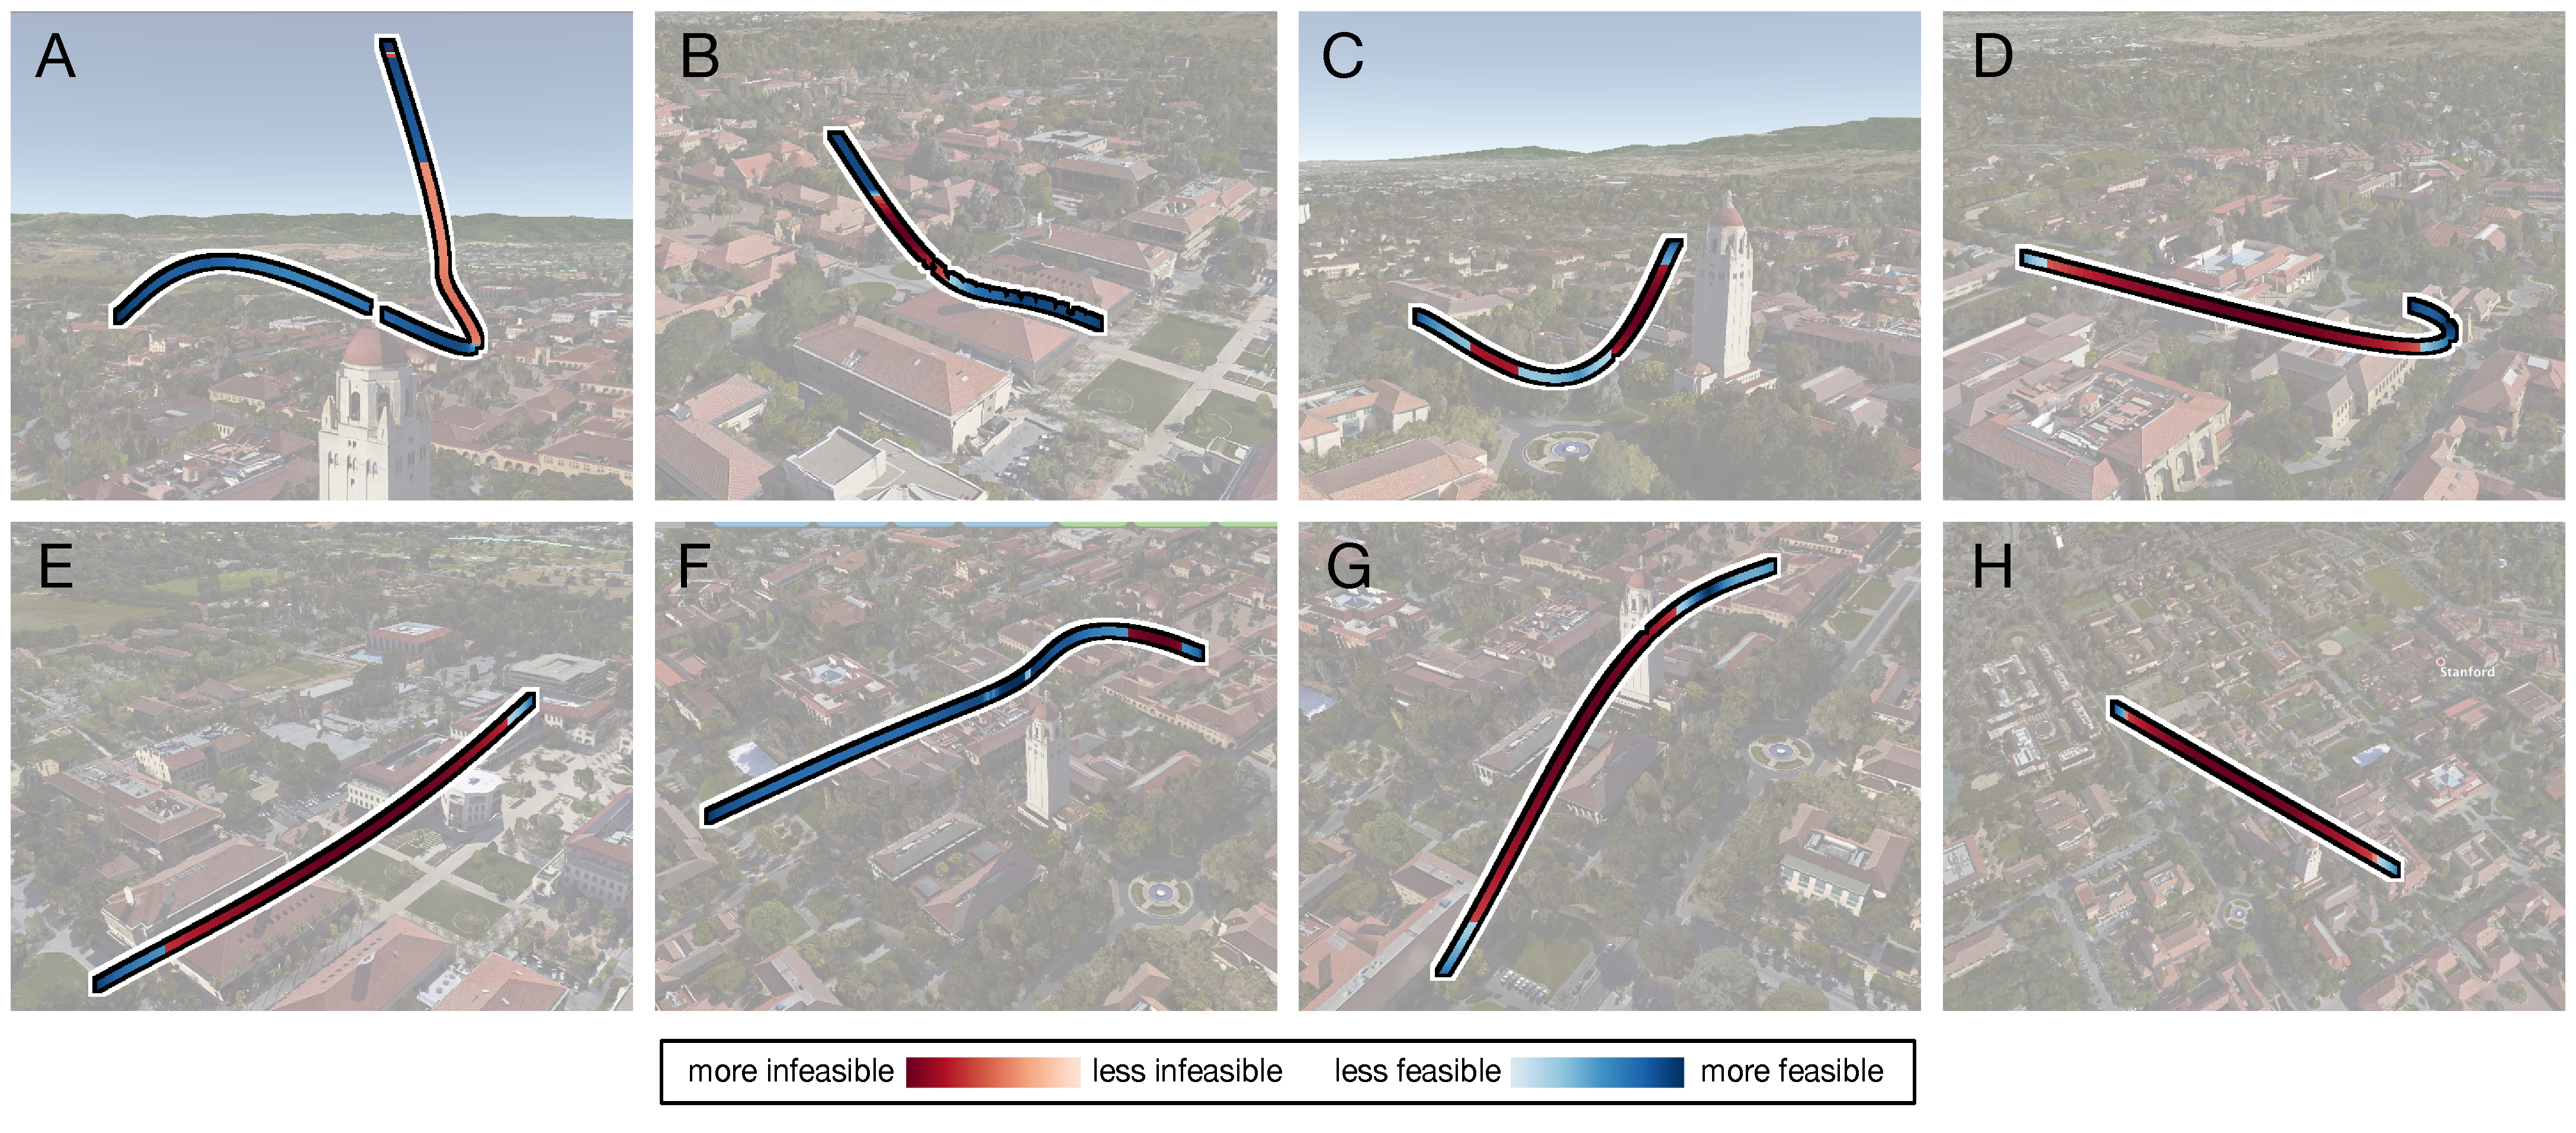
\includegraphics[width=6.0in]{images/2016_siggraph/03_dataset_24.pdf}
\caption{
Our dataset of infeasible quadrotor camera trajectories.
We show the trajectories in their spatial context, and color them according to how severely they violate our quadrotor's physical limits.
%Blue indicates regions of the trajectory that do not violate any constraints, and red indicates regions that violate at least one constraint.
%Deeper blue indicates regions that are further away from constraint boundaries, whereas deeper red indicates regions that more severely violate the constraints.
We use the letters in this figure to refer to individual trajectories throughout the paper.
}
\label{fig:ch3:dataset}
\end{figure*}

We based our dataset of infeasible quadrotor camera trajectories on raw data from the user study described in Chapter~\ref{sec:ch2}.
In this study, participants were tasked with creating cinematically interesting shots using \textsc{Horus}, an open source tool for quadrotor camera shot planning.
This study included 2 expert cinematographers, and 2 novice cinematographers with computer graphics experience.

\textsc{Horus} notifies users when their shots are infeasible, but requires users to manually edit their shots to make them feasible.
All of the shots from the previous study were infeasible at some point during the user's editing session.

\textsc{Horus} saves the complete revision history of a shot as it is being edited.
To compile our dataset, we simply found an infeasible revision for each shot in this previous study.
For the purpose of data collection, we assumed that revisions closer to the end of an editing session were more faithful to the user's artistic intent.
Therefore, as we compiled our dataset, we preferred revisions that were closer to end of an editing session. 
From this data collection procedure, we obtained 8 infeasible shots.
The feasibility violations in these shots ranged from moderate (e.g., briefly violating velocity limits by less than 10\%) to pronounced (e.g., violating velocity or control force limits by more than 50\% for sustained periods). 
We show the infeasible trajectories in our dataset in Figure~\ref{fig:ch3:dataset}.

\paragraph{Computational Performance}

To evaluate computational performance, we compared the running times of our algorithm and spacetime constraints on our dataset of infeasible trajectories.
We show the results from these experiments in Figure~\ref{fig:ch3:computation}.
%We describe the exact spacetime constraints problem formulation we use in our experiments in Appendix \ref{app:spacetime}.

In the interest of making fair comparisons, we took care to structure the implementations of our algorithm and spacetime constraints as similarly as possible.
The following implementation details apply to both implementations.
We solve the non-convex optimization problems arising in both approaches using the commercially available solver SNOPT~\cite{gill:2002}.
We initialize both approaches using the initialization strategy described in Section~\ref{sec:ch3:optimization}.
We call SNOPT using a Python wrapper provided by the authors, and we use all the default SNOPT error tolerances and parameters in all our experiments.
We express our objective function and constraint functions symbolically using the open-source symbolic algebra library SymPy~\cite{sympy:2014}.
We use SymPy to automatically generate all necessary gradient expressions. Finally, we use SymPy to generate efficient C code, which we call from Python, to evaluate the objective function, all constraint functions, and all necessary gradients.
We perform all our experiments on a Late 2013 Macbook Pro with a 2.6 GHz Intel Core i7 processor and 16GB of memory.

\paragraph{Convergence Behavior}

\begin{figure*}[t]
\centering
\includegraphics[width=6.0in]{images/2016_siggraph/00_computational_performance.pdf}
\caption{
Computational performance and scaling behavior of our algorithm on our dataset of infeasible trajectories.
When we solve for trajectories discretized at a moderate resolution of 100 time samples, our algorithm runs in less than 2 seconds, and is between 25$\times$ and 45$\times$ faster than spacetime constraints (a and b).
As we scale to more finely discretized trajectories, this performance gap widens, with our algorithm outperforming spacetime constraints by between 90$\times$ and 180$\times$ (c and d).
We indicate trajectories where spacetime constraints failed to find a solution with a $\star$.
We show the scaling behavior of our algorithm and spacetime constraints for trajectory \textsc{D}, which is the trajectory where spacetime constraints performed the best (e).
When scaling beyond 200 time samples, spacetime constraints did not consistently find a feasible solution for trajectory \textsc{D}.
We indicate where spacetime constraints successfully found a solution for trajectory \textsc{D} with colored dots.
%We take care to initialize our algorithm and spacetime constraints identically, using the initialization strategy described in Section \ref{sec:initialization}.
As a baseline, we include timing results for the modification of our algorithm described in Section~\ref{sec:ch3:results}.
On plots a, c, and e, lower is better.
}
\label{fig:ch3:computation}
\end{figure*}

\begin{figure}[t]
\centering
\includegraphics[width=4.0in]{images/2016_siggraph/01_convergence.pdf}
\caption{
Convergence behavior of our algorithm on trajectory \textsc{B} from our dataset of infeasible trajectories, discretized into 100 time samples.
This is the trajectory where spacetime constraints converged the fastest.
%We run SNOPT to convergence, using all the default SNOPT error tolerances and parameters. We indicate convergence with large colored dots.
Our algorithm, the modification of our algorithm described in Section~\ref{sec:ch3:results}, and spacetime constraints all converge rapidly to an optimal objective value (a).
However, because the equality constraints in our formulation are nearly linear, our algorithm converges to a solution that satisfies the equality constraints much faster than spacetime constraints (b).
We measure equality constraint error by summing the $l_2$ norm of each vector-valued equality constraint function, which is zero when the equality constraint is satisfied exactly. 
The y axes on these plots use a log scale.
Lower is better.
}
\label{fig:ch3:convergence}
\end{figure}

To evaluate the convergence behavior of our algorithm, we examined how the objective value in our optimization problem decreases as SNOPT makes progress towards an optimal solution for a trajectory in our dataset.
Similarly, we examined how the equality constraint functions, which are zero when the equality constraints are satisfied exactly, decrease as SNOPT makes progress.
Again, in all our experiments, we call SNOPT using all the default error tolerances and parameters.
We show the results from these experiments in Figure~\ref{fig:ch3:convergence}.

\paragraph{Accuracy}

\begin{figure}[t!]
\centering
\includegraphics[width=4.0in]{images/2016_siggraph/02_accuracy.pdf}
\caption{
Accuracy of our algorithm in predicting the results of a rigid body physics simulation.
We simulate the control trajectory produced by our algorithm using a \nth{5} order accurate rigid body simulator, and we measure how well the results of the simulation match the state space trajectory produced by our algorithm (a).
We repeat this experiment using the modification of our algorithm described in Section~\ref{sec:ch3:results} (b), spacetime constraints (c), and the original infeasible input trajectory simulated without control limits (d).
We plot the results for trajectory \textsc{G} in our dataset of infeasible trajectories, which was the trajectory where our algorithm performed the worst.
We provide mean error ($\mu$) and standard deviation ($\sigma$) values above each plot.
Even for this worst-case trajectory, our algorithm is more accurate than spacetime constraints, with slightly lower mean error.
For this particular trajectory, our unmodified algorithm is also slightly more accurate than our modified algorithm.
Having more histogram mass further to the left is better.
}
\label{fig:ch3:accuracy}
\end{figure}

To evaluate accuracy, we conducted an experiment using the state space and control trajectories produced by our algorithm.
%Our algorithm uses these state space and control trajectories to determine if the user's input camera trajectory has been slowed down enough to become feasible.
%Therefore, it is important that our algorithm produces accurate state space and control trajectories.
We simulated the control trajectories using a \nth{5} order accurate rigid body physics simulator, and we measured how well the results of the simulation matched the state space trajectories produced by our algorithm.
We repeated this experiment with spacetime constraints, the modified version of our algorithm, and the original infeasible input trajectory simulated without control force limits.
We show results from these experiments in Figure~\ref{fig:ch3:accuracy}.
Due to the relatively large time steps involved in these simulations, we applied LQR feedback control~\cite{tedrake:2016} in order to prevent the simulations from diverging.
We used identical LQR parameters in all our experiments.
We do not allow the LQR feedback controller to exceed the quadrotor's control force limits, except when simulating the infeasible input trajectories.

%To recover state space and control control trajectories from a speed profile produced by our algorithm, we simply evaluate the inequality constraint functions, $\mathbf{g}_\mathbf{x}$ and $\mathbf{g}_\mathbf{u}$, across the speed profile.
%We associate specific points along the speed profile with specific time values using the timing function computed in Section \ref{sec:optimization}.
%We recover state space and control trajectories for the original infeasible input trajectory using the algorithm presented in Section \ref{sec:control}.
%Spacetime constraints solves for state space and control trajectories explicitly, so no recovery procedure is needed to obtain these trajectories from spacetime constraints.

\paragraph{Dimensionality}

At each time sample, spacetime constraints requires at least 6 scalar decision variables for the configuration of the quadrotor, and 4 scalar decision variables for the quadrotor control forces.
In contrast, our formulation requires 5 scalar decision variables at each time sample.
Both formulations lead to the same block bi-diagonal structure in the constraint Jacobian.
Therefore, compared to spacetime constraints, our formulation reduces the required number of decision variables by at least 50\%, while preserving the efficient sparsity pattern in the constraint Jacobian.

\paragraph{Limitations}

By design, our algorithm will make an input trajectory feasible by perturbing its timing, but will not modify its spatial layout.
Therefore, our algorithm is not directly applicable in scenarios where the precise timing of the trajectory must be maintained.
In these scenarios, a spacetime constraints approach would be more appropriate.
That being said, we believe there is a broad class of usage scenarios in cinematography, journalism, and architecture, where re-timing an infeasible trajectory is reasonable behavior.
Therefore, we do not believe this limitation is overly burdensome.


\section{Conclusions}

We analyzed the dynamics of a quadrotor along a fixed path, and we found that the quadrotor's velocities and control forces are fully determined by its progress curve along the path.
This insight lead us to a fast and user-friendly algorithm for generating feasible quadrotor camera trajectories.
We implemented our algorithm in an open source tool for designing quadrotor camera shots, and we ran performance benchmarks on a dataset of infeasible quadrotor camera trajectories.
We found that our approach is between 25$\times$ and 180$\times$ faster than spacetime constraints.
We successfully captured real video footage using the trajectories generated by our algorithm.

In the future, we believe the ideas in this paper could become part of the standard toolbox for quadrotor trajectory planning.
By moving along networks of fixed paths, quadrotor cameras could film highly dynamic scenes with stronger safety guarantees.
By considering other objective functions along fixed paths, quadrotors could perform a wide range of tasks more efficiently and more safely.


% \appendix

\section{Defining the Quadrotor Camera Manipulator Matrices}
\label{appendix:manipulator}

In this appendix, we define the quadrotor camera manipulator matrices, attempting to be as concise as possible.
We include a detailed derivation of these matrices in the supplementary material.

We begin by defining the layout of our degree-of-freedom vector $\mathbf{q}$, and our control vector $\mathbf{u}$, as follows,
%
\footnotesize
\begin{equation}
\mathbf{q} = 
\begin{bmatrix}
\mathbf{p} \\
\mathbf{e}_q \\
\mathbf{e}_g
\end{bmatrix}
%
~~~~
\mathbf{u} = 
\begin{bmatrix}
\mathbf{u}_q \\
\mathbf{u}_g
\end{bmatrix}
\end{equation}
\normalsize
%
where $\mathbf{p}$ is the position of the quadrotor's center of mass; $\mathbf{e}_q$ is the vector of Euler angles representing the quadrotor's orientation in the world frame; $\mathbf{e}_g$ is the vector of Euler angles representing the orientation of the gimbal in the body frame of the quadrotor; $\mathbf{u}_q$ is the thrust control we apply at the quadrotor propellors; and $\mathbf{u}_g$ is the torque control we apply at the gimbal.

We express the manipulator matrices for our quadrotor camera system as follows,
%
\footnotesize
\begin{equation}
\begin{aligned}
\mathbf{H}(\mathbf{q}) = &
\begin{bmatrix}
m\mathbf{I}_{3\times3} & \mathbf{0}_{3\times3} & \mathbf{0}_{3\times3} \\
\mathbf{0}_{3\times3}                          & \mathbf{I}_{q} \mathbf{R}_{\mathcal{Q},\mathcal{W}} \mathbf{A}_q & \mathbf{0}_{3\times3} \\
\mathbf{0}_{3\times3}                          & \mathbf{0}_{3\times3} & \mathbf{A}_{g}
\end{bmatrix} \\
%
\mathbf{C}(\mathbf{q},\dot{\mathbf{q}}) = &
\end{aligned} \notag
\end{equation}
%
\vspace{-10pt}
\begin{equation}
\begin{aligned}
\begin{bmatrix}
\mathbf{0}_{3\times3} & \mathbf{0}_{3\times3}  & \mathbf{0}_{3\times3} \\
\mathbf{0}_{3\times3} & \mathbf{I}_q \mathbf{R}_{\mathcal{Q},\mathcal{W}} \dot{\mathbf{A}}_q - \left(\mathbf{I}_q \mathbf{R}_{\mathcal{Q},\mathcal{W}} \mathbf{A}_q \dot{\mathbf{e}}_q \right)_{\times}\mathbf{R}_{\mathcal{Q},\mathcal{W}} \mathbf{A}_q & \mathbf{0}_{3\times3} \\
\mathbf{0}_{3\times3} & \mathbf{0}_{3\times3}  & \dot{\mathbf{A}}_g
\end{bmatrix}
\end{aligned} \notag
\end{equation}
%
\begin{equation}
\begin{aligned}
\mathbf{G}(\mathbf{q}) = &
\begin{bmatrix}
-\mathbf{f}_e \\
\mathbf{0}_{3\times1} \\
\mathbf{0}_{3\times1} \\
\end{bmatrix} \\
%
\mathbf{B}(\mathbf{q}) = &
\begin{bmatrix}
\mathbf{R}_{\mathcal{W},\mathcal{Q}} \mathbf{M}_{\mathbf{f}}    & \mathbf{0}_{3\times3} \\
\mathbf{M}_{\mathbf{\tau}}                                      & \mathbf{0}_{3\times3} \\
\mathbf{0}_{3\times4}                                           & \mathbf{I}_{3\times3} \\
\end{bmatrix} ~~~~~~~~~~~~~\text{}
\end{aligned}
\end{equation}
%
\normalsize
where $m$ is the mass of the quadrotor camera;
$\mathbf{I}_q$ is the inertia matrix of the quadrotor camera;
$\mathbf{R}_{\mathcal{W},\mathcal{Q}}$ is the rotation matrix that represents the quadrotor's orientation in the world frame (i.e., the rotation matrix that maps vectors from the body frame of the quadrotor into the world frame);
$\mathbf{R}_{\mathcal{Q},\mathcal{W}}$ is the rotation matrix that maps vectors from the world frame into the body frame of the quadrotor;
$\mathbf{A}_q$ is the matrix that relates the quadrotor's Euler angle time derivatives to its angular velocity in the world frame;
$\mathbf{A}_g$ is the matrix that relates the gimbal's Euler angle time derivatives to its angular velocity in the body frame of the quadrotor;
$\mathbf{f}_e$ is the external force;
$\mathbf{M}_{\mathbf{f}}$ is the matrix that maps the control input at each of the quadrotor's propellers into a net thrust force oriented along the quadrotor's local $\mathbf{y}$ axis;
$\mathbf{M}_{\mathbf{\tau}}$ is the matrix that maps the control input at each of the quadrotor's propellers into a net torque acting on the quadrotor in the body frame;
$\mathbf{0}_{p \times q}$ is the $p \times q$ zero matrix;
$\mathbf{I}_{k \times k}$ is the $k \times k$ identity matrix;
and the notation $\left( \mathbf{a} \right)_{\times}$ refers to the skew-symmetric matrix, computed as a function of the vector $\mathbf{a}$, such that $\left(\mathbf{a}\right)_{\times}\mathbf{b} = \mathbf{a}\times\mathbf{b}$ for all vectors $\mathbf{b}$.

Our expressions for the quadrotor camera manipulator matrices depend on the matrices, $\mathbf{M}_{\mathbf{f}}$ and $\mathbf{M}_{\mathbf{\tau}}$.
We define these matrices as follows, 
%
\footnotesize
\begin{equation}
\begin{aligned}
%
\mathbf{M}_{\mathbf{f}} = &
\begin{bmatrix}
0 & 0 & 0 & 0 \\
1 & 1 & 1 & 1 \\
0 & 0 & 0 & 0 \\
\end{bmatrix}\\
%
\mathbf{M}_{\mathbf{\tau}} = &
\begin{bmatrix}
 ds_\alpha & ds_\beta & -ds_\beta & -ds_\alpha \\
\gamma     & -\gamma  & \gamma    & -\gamma    \\
-dc_\alpha & dc_\beta & dc_\beta  & -dc_\alpha \\
\end{bmatrix}
%
\end{aligned}
\end{equation}
\normalsize
%%
where $d$, $\alpha$, $\beta$, and $\gamma$ are constants related to the physical design of a quadrotor:
$d$ is the distance from the quadrotor's center of mass to its propellers;
$\alpha$ is the angle in radians that the quadrotor's front propellers form with the quadrotor's positive $\mathbf{x}$ axis;
$\beta$ is the angle in radians that the quadrotor's rear propellers form with the quadrotor's negative $\mathbf{x}$ axis;
$\gamma$ is the magnitude of the in-plane torque generated by the quadrotor propeller producing 1 unit of upward thrust force;
$c_a=\cos a$ and $s_a=\sin a$.

Note that our expressions for the quadrotor camera manipulator matrices, in particular our expressions for $\mathbf{A}_q$ and $\mathbf{A}_g$, depend on our choice of Euler angle conventions.
See our derivation in the supplementary material for details.

%Our expressions for the quadrotor camera manipulator matrices also depend on our choice of Euler angle conventions.
%Throughout this paper, we adopt the following Euler angle conventions.
%Let $\mathbf{e} = [ \theta ~ \psi ~ \phi ]^T$ be a vector of Euler angles, and let $\omega$ be angular velocity in the non-rotating frame as these Euler angles change over time. We define the corresponding rotation matrix $\mathbf{R}$ in terms of the Euler angles $\theta$, $\psi$, and $\phi$ as follows,
%%
%\footnotesize
%\begin{equation}
%\begin{aligned}
%%
%\mathbf{R} & = \mathbf{R}_{\mathbf{y}}^{\psi} \mathbf{R}_{\mathbf{z}}^{\theta} \mathbf{R}_{\mathbf{x}}^{\phi} \\
%& = 
%\begin{bmatrix}
%c_\psi  & 0 & s_\psi \\
%0       & 1 & 0 \\
%-s_\psi & 0 & c_\psi \\
%\end{bmatrix}
%\begin{bmatrix}
%1 & 0        & 0 \\
%0 & c_\theta & -s_\theta \\
%0 & s_\theta & c_\theta \\
%\end{bmatrix}
%%
%\begin{bmatrix}
%c_\phi & -s_\phi & 0 \\
%s_\phi & c_\phi  & 0 \\
%0      & 0       & 1 \\
%\end{bmatrix}
%%
%\end{aligned}
%\end{equation}
%\normalsize
%%
%where $c_a=\cos a$ and $s_a=\sin a$.
%Finally, we define the matrix $\mathbf{A}$ that relates $\dot{\mathbf{e}}$ to $\omega$ according to the linear relationship $\mathbf{A} \dot{\mathbf{e}} = \omega$, and its time derivative $\dot{\mathbf{A}}$, as follows,
%%
%\footnotesize
%\begin{equation}
%\begin{aligned}
%%
%\mathbf{A} & =
%\begin{bmatrix}
%c_\psi  & 0 & s_\psi c_\theta \\
%0       & 1 & -s_\theta       \\
%-s_\psi & 0 & c_\psi c_\theta \\
%\end{bmatrix} \\
%%
%\dot{\mathbf{A}} & =
%\begin{bmatrix}
%-s_\psi \dot{\psi} & 0 & -s_\psi s_\theta \dot{\theta} + c_\psi c_\theta \dot{\psi} \\
%0                  & 0 & -c_\theta \dot{\theta} \\
%-c_\psi \dot{\psi} & 0 & -s_\psi c_\theta \dot{\psi} + s_\theta c_\psi \dot{\theta} \\
%\end{bmatrix}
%%
%\end{aligned}
%\end{equation}
%\normalsize
%%
%where $c_a=\cos a$ and $s_a=\sin a$.


\chapter{Submodular Trajectory Optimization for Aerial 3D Scanning}

\input{04_2017_iccv/00_abstract}
% \section{Introduction}

Small consumer drones equipped with high-resolution cameras are emerging as a powerful tool for large-scale aerial 3D scanning.
In order to obtain high-quality 3D reconstructions, a drone must capture images that densely cover the scene.
Additionally, 3D reconstruction methods typically require surfaces to be viewed from multiple viewpoints, at an appropriate distance, and with sufficient angular separation (i.e., baseline) between views.
%These constraints require users to carefully plan trajectories or carefully maneuver the drone which requires experience and skill.
Existing autonomous flight planners do not always satisfy these  requirements, which can be difficult to reason about, even for a skilled human pilot manually controlling a drone.
Furthermore, the limited battery life of consumer drones provides only 10--15 minutes of flight time, making it even more challenging to obtain high-quality 3D reconstructions.

%The proliferation of inexpensive, high quality cameras along increasingly commoditized aerial platforms (drones), have made it easier %to capture and model large 3D environments using structure-from-motion (SfM) and multi-view stereo (MVS) methods.
%However, ensuring a high quality reconstruction with good coverage with reasonable capture and reconstruction times is not trivial.
%The quality of a reconstruction is a function of the number of images, the spacing between the sampled camera poses (baselines), the distance to surfaces in the scene, and the amount of the scene that has been viewed \cite{hornung:2008}.
%Controlling a drone to optimize these properties is very challenging, even for an experienced pilot, especially given the hard constraints posed by the limited battery life of a drone, which can limit captures to only minutes.
%As a result, drone-based scene capture can require many flights to ensure quality and coverage, or alternatively one must sacrifice quality and coverage.

In lieu of manual piloting, commercial flight planning tools generate conservative trajectories (e.g., a lawnmower or orbit pattern at a safe height above the scene) that attempt to cover the scene while respecting flight time budgets \cite{3dr:2017a,pix4d:2017a}.
However, because these trajectories are generated with no awareness of the scene geometry, they tend to over-sample some regions (e.g., rooftops), while under-sampling others (e.g., facades, overhangs, and fine details), and therefore sacrifice reconstruction quality.

In this chapter, we introduce a method to automate aerial 3D scanning, by planning good camera trajectories for reconstructing large 3D scenes (see Figure \ref{fig:ch1:teaser_ch4}).
Our method relies on a mathematical model that evaluates the usefulness of a camera trajectory for the purpose of 3D scanning.
Given a coarse estimate of the scene geometry as input, our model quantifies how well a trajectory covers the scene, and also quantifies the diversity and appropriateness of views along the trajectory.
Using this model for scene coverage, our method generates trajectories that maximize coverage, subject to a travel budget.
We bootstrap our method using coarse scene geometry, which we obtain using the imagery acquired from a short initial flight over the scene. 

%Subsequently, we fly our optimized trajectory, and we use the additional imagery from our optimized flight to reconstruct the high-fidelity scene during post-processing.
%As our experiments show, this strategy improves the completeness and visual quality of our reconstructed 3D models.

%In particular, our approach is designed to account for the domain-specific requirements of modern 3D reconstruction algorithms, i.e., we aim to maximize the area covered by all camera locations, across all surface points, subject to a budget to account for the limited flying time of a drone. We perform the optimization by bootstrapping with a geometry estimate from a simple short flight that we used to planning a new trajectory. After flying this new trajectory the images acquired are added to the 3D reconstruction process to refining the geometry from the initial short flight, ultimately yielding higher-quality 3D reconstructions than would be possible to obtain otherwise.

We formulate our trajectory planning task as a reward-collecting graph optimization problem known as \textit{orienteering}, that combines aspects of the traveling salesman and knapsack problems, and is known to be NP-hard \cite{gunawan:2016,vansteenwegena:2011}.
However, unlike the additive rewards in the standard orienteering problem, our rewards are non-additive, and globally coupled through our coverage model.
We make the observation that our coverage model exhibits an intuitive diminishing returns property known as \textit{submodularity} \cite{krause:2014}, and therefore we must solve a \textit{submodular orienteering} problem.
Although submodular orienteering is strictly harder than additive orienteering, it exhibits useful structure that can be exploited.
We propose a novel transformation of our submodular orienteering problem into an additive orienteering problem, and we solve the additive problem as an integer linear program. We leverage submodularity extensively throughout the derivation of our method, to obtain approximate solutions with strong theoretical guarantees, and dramatically reduce computation times.

We demonstrate the utility of our method by using it to scan three large outdoor scenes: a barn, an office building, and an industrial site.
We also quantitatively evaluate our algorithm in a photorealistic video game simulator.
In all our experiments, we obtain noticeably higher-quality 3D reconstructions than strong baseline methods.
% CUTTING TO SHORTEN -- that works well for MVS algorithms.
%
%which we exploit throughout our method to obtain strong approximation guarantees and significantly reduce computation times.

%% THIS FOLLOWING SENTENCE DOES NOT ADD MUCH !
%We evaluate our algorithm quantitatively using a photorealistic game engine and use it to scan three large outdoor scenes. We show that our method consistently recovers more
%complete 3D models with higher resolution texture maps compared to existing methods.

%We demonstrate the utility of our algorithm by using it to scan three large outdoor scenes: a barn, an office building, and an industrial site. We also quantitatively

\vspace{-5pt}
\section{Related Work}

\paragraph{Aerial 3D Scanning and Mapping}
High-quality 3D reconstructions of very large scenes can be obtained using offline multi-view stereo algorithms \cite{furukawa:2015} to process images acquired by drones \cite{pix4d:2015}.
Real-time mapping algorithms for drones have also been proposed, that take as input either RGBD \cite{heng:2011,loianno:2015,michael:2012,sturm:2013} or RGB \cite{wendel:2012} images, and produce as output a 3D\ reconstruction of the scene.
These methods are solving a reconstruction problem, and do not, themselves, generate drone trajectories.
Several commercially available flight planning tools have been developed to assist with 3D scanning \cite{3dr:2017a,pix4d:2017a}.
However, these tools only generate conservative lawnmower and orbit trajectories above the scene.
In contrast, our algorithm generates trajectories that cover the scene as thoroughly as possible, ultimately leading to higher-quality 3D reconstructions.

Generating trajectories that \emph{explore} an unknown environment, while building a map of it, is a classical problem in robotics \cite{thrun:2005}.
Exploration algorithms have been proposed for drones based on local search heuristics \cite{stumberg:2016}, identifying the frontiers between known and unknown parts of the scene \cite{heng:2014,shen:2012}, maximizing newly visible parts of the scene \cite{bircher:2016}, maximizing information gain \cite{charrow:2015b,charrow:2015a}, and imitation learning \cite{choudhury:2017}.
A closely related problem in robotics is generating trajectories that \emph{cover} a known environment \cite{galceran:2013}.
Several coverage path planning algorithms have been proposed for drones \cite{alexis:2015,bircher:2015,heng:2015,hollinger:2013}.
In an especially similar spirit to our work, Heng et al.~propose to reconstruct an unknown environment by executing alternating exploration and coverage trajectories \cite{heng:2015}.
However, existing strategies for exploration and coverage do not explicitly account for the domain-specific requirements of multi-view stereo algorithms (e.g., observing the scene geometry from a diverse set of viewing angles).
Moreover, existing exploration and coverage strategies have not been shown to produce visually pleasing multi-view stereo reconstructions, and are generally not evaluated on multi-view stereo reconstruction tasks.
In contrast, our trajectories cover the scene in a way that explicitly accounts for the requirements of multi-view stereo algorithms, and we evaluate the multi-view stereo reconstruction performance of our algorithm directly.

Several path planning algorithms have been proposed for drones, that explicitly attempt to maximize multi-view stereo reconstruction performance \cite{dunn:2009a,hoppe:2012,mostegel:2016,schmid:2012}.
These algorithms are similar in spirit to ours, but adopt a two phase strategy for generating trajectories.
In the first phase, these algorithms select a sequence of \emph{next-best-views} to visit, ignoring travel costs.
In the second phase, they find an efficient path that connects the previously selected views.
In contrast, our algorithm reasons about these two problems -- selecting good views and routing between them -- jointly in a unified global optimization problem, enabling us to generate more rewarding trajectories, and ultimately higher-quality 3D\ reconstructions.

\vspace{-13pt}
\paragraph{View Selection and Path Planning}
The problem of optimizing the placement (and motion) of sensors to improve performance on a perception task is a classical problem in computer vision and robotics, where it generally goes by the name of \emph{active vision}, e.g., see the comprehensive surveys \cite{chen:2011,scott:2003,tarabanis:1995}.
We discuss directly related work not included in these surveys here.
A variety of active algorithms for 3D scanning with ground-based range scanners have been proposed, that select a sequence of next-best-views \cite{krainin:2011}, and then find an efficient path to connect the views \cite{fan:2016,wu:2014}.
In a similar spirit to our work, Wang et al.~propose a unified optimization problem that selects rewarding views, while softly penalizing travel costs \cite{wang:2007}.
We adapt these ideas to account for the domain-specific requirements of multi-view stereo algorithms, and we impose a hard travel budget constraint, which is an important safety requirement when designing drone trajectories.

Several algorithms have been proposed to select an appropriate subset of views for multi-view stereo reconstruction \cite{dunn:2009b,hornung:2008,mauro:2014b,mauro:2014a}, and to optimize coverage of a scene \cite{ghanem:2015,mavrinac:2013}.
However, these methods do not model travel costs between views.
In contrast, we impose a hard constraint on the travel cost of the path formed by the views we select.

\vspace{-14pt}
\paragraph{Submodular Path Planning}
Submodularity \cite{krause:2014} has been considered in path planning scenarios before, first in the theory community \cite{chekuri:2012,chekuri:2005}, and more recently in the artificial intelligence \cite{singh:2009a,singh:2009b,zhang:2016} and robotics \cite{heng:2015,hollinger:2013} communities.
The coverage path planning formulation of Heng et al.~\cite{heng:2015} is similar to ours, in the sense that both formulations use the same technique for approximating coverage \cite{iyer:2013b,iyer:2013a}.
We extend this formulation to account for the domain-specific requirements of multi-view stereo algorithms, and we evaluate the multi-view stereo reconstruction performance of our algorithm directly.

\vspace{-5pt}
\section{Technical Overview}
\label{sec:overview}

In order to generate scanning trajectories, our algorithm leverages a coarse estimate of the scene geometry.
Initially, we do not have any estimate of the scene geometry, so we adopt an \emph{explore-then-exploit} approach.

In the \emph{explore} phase, we fly our drone (i.e., we command our drone to fly autonomously) along a default trajectory at a safe distance above the scene, acquiring a sequence of images as we are flying.
We land our drone, and subsequently feed the acquired images to an open-source multi-view stereo pipeline, thereby obtaining a coarse estimate of the scene geometry, and  a strictly conservative estimate of the scene's free space.
We include a more detailed discussion of our \emph{explore} phase in the supplementary material.

In the \emph{exploit} phase, we use this additional information about the scene to plan a scanning trajectory that attempts to maximize the fidelity of the resulting 3D reconstruction.
At the core of our planning algorithm, is a coverage model that accounts for the domain-specific requirements of multi-view stereo reconstruction (Section \ref{sec:coverage_model}).
Using this model, we generate a scanning trajectory that maximizes scene coverage, while respecting the drone's limited flight time (Section \ref{sec:trajectories}). 
We fly the drone along our scanning trajectory, acquiring another sequence of images.
Finally, we land our drone again, and we feed all the images we have acquired to our multi-view stereo pipeline to obtain a detailed 3D reconstruction of the scene.

\begin{figure}[t]
\begin{center}
\includegraphics[width=0.47\textwidth]{images/2017_iccv/coverage_model_horizontal.pdf}{\vspace{-7pt}}
\end{center}
\caption{
Our coverage model for quantifying the usefulness of camera trajectories for multi-view stereo reconstruction. More useful trajectories cover more of the hemisphere of viewing angles around surface points.
(a) An illustrative example showing coverage of a single surface point with three cameras. Each camera covers a circular disk on a hemisphere around the surface point $\mathbf{s}$, and the total solid angle covered by all the disks determines the total usefulness of the cameras.
Note that the angular separation (i.e., baseline) between cameras $\mathbf{c}_2$ and $\mathbf{c}_3$ is small and leads to diminishing returns in their combined usefulness.
(b) The usefulness of a camera trajectory, integrated over multiple surface points, is determined by summing the total covered solid angle for each of the individual surface points. Our model naturally encourages diverse observations of the scene geometry, and encodes the eventual diminishing returns of additional observations.
\vspace{-10pt}
}
\label{fig:coverage_model}
\end{figure}
%
\begin{figure*}[t]
\begin{center}
\includegraphics[width=1.0\textwidth]{images/2017_iccv/algorithm_overview.pdf}{\vspace{-10pt}}
\end{center}
\caption{
Overview of our algorithm for generating camera trajectories that maximize coverage.
(a) Our goal is to find the optimal closed path of camera poses through a discrete graph.
(b) We begin by solving for the optimal camera orientation at every node in our graph, ignoring path constraints.
(c) In doing so, we remove the choice of camera orientation from our problem, coarsening our problem into a more standard form.
(d) The solution to the problem in (b) defines an approximation to our coarsened problem, where there is an additive reward for visiting each node.
(e) Finally, we solve for the optimal closed path on the additive approximation defined in (d).
\vspace{-10pt}
}
\label{fig:algorithm_overview}
\end{figure*}

\vspace{-5pt}
\section{Coverage Model for Camera Trajectories}
\label{sec:coverage_model}

In this section, we model the usefulness of a camera trajectory for multi-view stereo reconstruction, in terms of how well it covers the scene geometry.
We provide an overview of our coverage model in Figure \ref{fig:coverage_model}.

In reality, the most useful camera trajectory is the one that yields the highest-quality 3D reconstruction of the scene.
However, it is not clear how we would search for such a camera trajectory directly, without resorting to flying candidate trajectories and performing expensive 3D reconstructions for each of them.
In contrast, our coverage model only roughly approximates the true usefulness of a camera trajectory. 
However, as we will see in the following section, our coverage model: (1) is motivated by established best practices for multi-view stereo image acquisition; (2) is easy to evaluate; (3) only requires a coarse estimate of the scene geometry as input;  and (4) exhibits submodular structure, which will enable us to efficiently maximize it.

\vspace{-10pt}
\paragraph{Best Practices for Multi-View Stereo Image Acquisition}
As a rule of thumb, it is recommended to capture an image every 5--15 degrees around an object, and it is generally accepted that capturing images more densely will eventually lead to diminishing returns in the fidelity of the 3D reconstruction \cite{furukawa:2015}.
Similarly, close-up and fronto-parallel views can help to resolve fine geometric details, because these views increase the effective resolution of estimated depth images, and contribute more reliable texture information to the reconstruction \cite{waechter:2014}.
We explicitly encode these best practices for multi-view stereo image acquisition into our coverage model.

\vspace{-10pt}
\paragraph{Formal Definition}
Given a candidate camera trajectory and approximate scene geometry as a triangle mesh, our goal is to quantify how well the trajectory covers the scene geometry.
We first uniformly sample the camera trajectory to generate a discrete set $C$, consisting of individual camera poses $\mathbf{c}_{0:I}$.
Similarly, we uniformly sample oriented surface points $\mathbf{s}_{0:J}$ from the scene geometry.
For each oriented surface point $\mathbf{s}_j$, we define an oriented hemisphere $H_j$ around it.
For each surface point $\mathbf{s}_j$ and camera $\mathbf{c}_i$, we define a circular disk $D^j_i$ that covers an angular region of the hemisphere $H_j$, centered at the location where $\mathbf{c}_i$ projects onto $H_j$ (see Figure \ref{fig:coverage_model}).
When the surface point $\mathbf{s}_j$ is not visible from the camera $\mathbf{c}_i$, we define the disk $D^j_i$ to have zero radius, and we truncate the extent of each disk so that it does not extend past the equator of $H_j$.
We define the total covered region of the hemisphere $H_j$ as the union of all the disks that partially cover $H_j$ (see Figure \ref{fig:coverage_model}), referring to this total covered region as $V_j = \bigcup_{i=0}^I D^j_i$.
We define our coverage model as follows,
%
\begin{equation}
\begin{aligned}
f(C) = \sum_{j=0}^{J} \int_{V_j} w_j(\mathbf{h}) d\mathbf{h}
\end{aligned}
\label{eqn:model_irregular}
\end{equation}
%
where the outer summation is over all hemispheres; $\int_{V_j} d\mathbf{h}$ refers to the surface integral over the covered region $V_j$; and $w_j(\mathbf{h})$ is a non-negative weight function that assigns different reward values for covering different parts of $H_j$.
Our model can be interpreted as quantifying how well a set of cameras covers the scene's \emph{surface light field} \cite{davis:2012,wood:2000}.
We include a method for efficiently evaluating our coverage model in the supplementary material.

To encourage close-up views, we set the radius of $D^j_i$ to decay exponentially as the camera $\mathbf{c}_i$ moves away from the surface point $\mathbf{s}_j$. To encourage fronto-parallel views, we design each function $w_j(\mathbf{h})$ to decay in a cosine-weighted fashion, as the hemisphere location $\mathbf{h}$ moves away from the hemisphere pole.
We include our exact formulation for $D^j_i$ and $w_j(\mathbf{h})$ in the supplementary material.

\vspace{-10pt}
\paragraph{Submodularity}
Roughly speaking, a set function is submodular if the marginal reward for adding an element to the input set always decreases, as more elements are added to the input set \cite{krause:2014}.
Our coverage model is submodular, because all coverage functions with non-negative weights are submodular \cite{krause:2014}.
Submodularity is a useful property to identify when attempting to optimize a set function, and is often referred to as the discrete analogue of convexity.
We will leverage submodularity extensively in the following section, as we derive our algorithm for generating camera trajectories that maximizing coverage. 

\vspace{-5pt}
\section{Generating Optimal Camera Trajectories}
\label{sec:trajectories}
We provide an overview of our algorithm in Figure \ref{fig:algorithm_overview}.
Our approach is to formulate a reward-collecting optimization problem on a graph.
The nodes in the graph represent camera positions, the edges represent Euclidean distances between camera positions, and the rewards are collected by visiting new nodes.
The goal is to find a path that collects as much reward as possible, subject to a budget constraint on the total path length.
This general problem is known as the \emph{orienteering problem} \cite{gunawan:2016,vansteenwegena:2011}.

A variety of approaches have been proposed to approximately solve the orienteering problem, which is NP-hard.
However, these methods are not directly applicable to our problem, because they assume that the rewards on nodes are additive.
But the total reward we collect in our problem is determined by our coverage model, which does not exhibit additive structure.
Indeed, the marginal reward we collect at a node might be very large, or very small, depending on the entire set of other nodes we visit.


The marginal reward we collect at each node also depends strongly on the orientation of our camera. In other words, our orienteering problem involves extra choices -- how to orient the camera at each visited node -- and these choices are globally coupled through our submodular coverage function. Therefore, even existing algorithms for \emph{submodular orienteering} \cite{chekuri:2012,chekuri:2005,heng:2015,singh:2009a,singh:2009b,zhang:2016} are not directly applicable to our problem, because these algorithms assume there are no extra choices to make at each visited node.

Our strategy will be to apply two successive problem transformations.
First, we leverage submodularity to solve for the approximately optimal camera orientation at every node in our graph, ignoring path constraints (Fig.~\ref{fig:algorithm_overview}b, Section \ref{sec:trajectories_orientation}).
In doing so, we remove the choice of camera orientation from our orienteering problem, thereby coarsening it into a more standard form (Fig.~\ref{fig:algorithm_overview}c).
Second, we leverage submodularity to construct a tight additive approximation of our coverage function (Fig.~\ref{fig:algorithm_overview}d, Section \ref{sec:trajectories_subgradient}).
In doing so, we relax our coarsened submodular orienteering problem into a standard additive orienteering problem.
We formulate this additive orienteering problem as a compact integer linear program, and solve it approximately using a commercially available solver (Fig.~\ref{fig:algorithm_overview}e, Section \ref{sec:trajectories_ilp}).

\vspace{-10pt}
\paragraph{Preprocessing}
We begin by constructing a discrete set of all the possible camera poses we might include in our path.
We refer to this set as our \emph{ground set} of camera poses, $C$.
We construct this set by uniformly sampling a user-defined bounding box that spans the scene, then uniformly sampling a downward-facing unit hemisphere to produce a set of look-at vectors that our drone camera can actuate. We define our ground set as the Cartesian product of these positions and look-at vectors.
We construct the graph for our orienteering problem as the grid graph of all the unique camera positions in $C$, pruned so that it is entirely restricted to the known free space in the scene  (see Section \ref{sec:overview}).

\vspace{-10pt}
\paragraph{Our Submodular Orienteering Problem}
Let $\mathbf{P} = (\mathbf{p}_0, \mathbf{v}_0), (\mathbf{p}_1, \mathbf{v}_1), \ldots, (\mathbf{p}_q, \mathbf{v}_q)$ be a camera path through our graph, represented as a sequence of camera poses taken from our ground set.
We represent each camera pose as a position $\mathbf{p}_i$ and a look-at vector $\mathbf{v}_i$.
We would like to find the optimal path $\mathbf{P}^{\star}$ as follows,
%
\begin{equation}
\begin{aligned}
\mathbf{P}^{\star} = \argmax_{\mathbf{P}} f(C_{\mathbf{P}})~~~~~~~~~~~~~~~~\\
\text{subject to} ~~~~~ l(\mathbf{P}) \leq B ~~~~~ \mathbf{p}_0 = \mathbf{p}_q = \mathbf{p}_\text{root}
\end{aligned}
\label{eqn:submodular_orienteering}
\end{equation}
%
where
$C_\mathbf{P} \subseteq C$ is the set of all the unique camera poses along the path; 
$l(\mathbf{P})$ is the length of the path; $B$ is a user-defined travel budget; and $\mathbf{p}_\text{root}$ is the position where our path must start and end.
For safety reasons, we would also like to design trajectories that consume close to, but no more than, some fixed fraction of our drone's battery (e.g., 80\% or so). However, constraining battery consumption directly is difficult to express in our orienteering formulation, so we model this constraint indirectly by imposing a budget constraint on path length.
We make the observation that our problem is intractable in its current form, because it requires searching over an exponential number of paths through our graph. This observation motivates the following two problem transformations.

\subsection{Solving for Optimal Camera Orientations} 
\label{sec:trajectories_orientation}

Our goal in this subsection is to solve for the optimal camera orientation at every node in our graph, ignoring path constraints. 
We achieve this goal with the following relaxation of the problem in equation (\ref{eqn:submodular_orienteering}).
Let $C_S \subseteq C$ be a subset of camera poses from our ground set. We would like to find the optimal subset of camera poses  $C_S^{\star}$ as follows,
%
\begin{equation}
\begin{aligned}
C_S^{\star} = \argmax_{C_S} f(C_S)~~~~~~~~~\\
\text{subject to} ~~~~~ \left\vert C_S \right\vert = N ~~~~~ C_S \in \mathcal{M}
\end{aligned}
\label{eqn:cardinality_matroid}
\end{equation}
%
where
$\left\vert C_S \right\vert$ is the cardinality of $C_S$;
$N$ is the total number of unique positions in our graph;
and the constraint $C_S \in \mathcal{M}$ enforces mutual exclusion, where we are allowed to select at most one camera orientation at each node in our graph.
In this relaxed problem, we are attempting to maximize coverage by selecting exactly one camera orientation at each node in our graph.
We can interpret such a solution as a coarsened ground set for the problem in equation (\ref{eqn:submodular_orienteering}), thereby transforming it into a standard submodular orienteering problem.

Because our coverage function is submodular, the problem in equation (\ref{eqn:cardinality_matroid}) can be solved very efficiently, and to within 50\% of global optimality, with a very simple greedy algorithm \cite{krause:2014}.
Roughly speaking, the greedy algorithm selects camera poses from our ground set in order of marginal reward, taking care to respect the mutual exclusion constraint, until no more elements can be selected.
Submodularity can also be exploited to significantly reduce the computation time required by the greedy algorithm (e.g., from multiple hours to a couple of minutes, for the problems we consider in this paper) \cite{krause:2014}.
The approximation guarantee in this subsection relies on the fact that selecting more camera poses never reduces coverage, i.e., our coverage function exhibits a property known as \emph{monotonicity} \cite{krause:2014}.
We include a more detailed discussion of the greedy algorithm, and provide pseudocode, in the supplementary material.

\subsection{Additive Approximation of Coverage}
\label{sec:trajectories_subgradient}

Our goal in this subsection is to construct an additive approximation of coverage.
In other words, we would like to define an additive reward at each node in our graph, that closely approximates our coverage function for arbitrary subsets of visited nodes.

To construct our additive approximation, we draw inspiration from the approach of Iyer et al.~\cite{iyer:2013b,iyer:2013a}.
We begin by choosing a permutation of elements in our coarsened ground set.
Let $\mathbf{C} = \mathbf{c}_0, \mathbf{c}_1, \ldots, \mathbf{c}_N$ be our permutation, where $\mathbf{c}_i$ is the $i^{\text{th}}$ element of our coarsened ground set in permuted order.
Let $C_i = \{ \mathbf{c}_0, \mathbf{c}_1, \ldots, \mathbf{c}_{i-1} \}$ be the subset containing the first $i$ elements of our permutation.
We define the additive reward for each element in our permutation as $\tilde{f}_i = f(C_i \cup \mathbf{c}_i) - f(C_i)$.
For an arbitrary subset $C_S$, our additive approximation is simply the sum of additive rewards for each element in $C_S$. Due to submodularity, this additive approximation is guaranteed to be exact for all subsets $C_i$, and to underestimate our true coverage function for all other subsets.
This guarantee is useful for our purposes, because any solution we get from optimizing our additive approximation will yield an equal or greater reward on our true coverage function.

When choosing a permutation, it is generally advantageous to place camera poses with the greatest marginal reward at the front of our permutation.
With this intuition in mind, we form our permutation by sorting the camera poses in our coarsened ground set according to their marginal reward.
Fortunately, we have already computed this ordering in Section \ref{sec:trajectories_orientation} using the greedy algorithm.
So, we simply reuse this ordering to construct our additive approximation.

\subsection{Orienteering as an Integer Linear Program}
\label{sec:trajectories_ilp}

After constructing our additive approximation of coverage, we obtain the following additive orienteering problem, 
%
\begin{equation}
\begin{aligned}
\mathbf{P}^{\star} = \argmax_{\mathbf{P}} \sum_{C_{\mathbf{P}}} \tilde f_i~~~~~~~~~~~~~~~\\
\text{subject to} ~~~~~ l(\mathbf{P}) \leq B ~~~~~ \mathbf{p}_0 = \mathbf{p}_q = \mathbf{p}_\text{root}
\end{aligned}
\label{eqn:ilp}
\end{equation}
%
where $\tilde f_i$ is the additive reward for each unique      node along the path $\mathbf{P}$.
In its current form, it is still not clear how to solve this problem efficiently, because we must still search over an exponential number of paths through our graph.
Fortunately, we can express this problem as a compact integer linear program, using a formulation suggested by Letchford et al.~\cite{letchford:2013}.
We transform our undirected graph into a directed graph, and we define integer variables to represent if nodes are visited and directed edges are traversed.
Remarkably, we can constrain the configuration of these integer variables to form only valid paths through our graph, with a compact set of linear constraints.
We include a more detailed derivation of this formulation in the supplementary material.

Leveraging the formulation suggested by Letchford et al., we convert the problem in equation (\ref{eqn:ilp}) into a standard form that can be given directly to an off-the-shelf solver.
We use the modeling language CVXPY \cite{cvxpy:2016} to specify our problem, and we use the commercially available Gurobi Optimizer \cite{gurobi:2017} as the back-end solver.
Solving integer programming problems to global optimality is NP-hard, and can take a very long time, so we specify a solver time limit of 5 minutes.
Gurobi returns the best feasible solution it finds within the time limit, along with a worst-case optimality gap.
In our experience, Gurobi consistently converges to a close-to-optimal solution in the allotted time (i.e., typically with an optimality gap of less than 10\%).
At this point, the resulting orienteering trajectory can be safely and autonomously executed on our drone.

%%MOVE THIS TO APPENDIX
%We replace each undirected edge in our graph with two directed \emph{arcs}, each with the same cost as the original undirected edge.
%We define the indicator vectors $\mathbf{x}$ and $\mathbf{y}$ to represent whether or not each arc is traversed and
%whether or not each node in our graph is visited respectively. Also let vector $\mathbf{g}$ contain the cumulative costs incurred so far, when beginning to traverse each arc. Finally, we define the constant vector $\mathbf{f}$ to contain the additive reward at each each node, and a constant vector $\mathbf{r}$ to contain the instantaneous cost of traversing each arc.

%We also define inbound and outbound \emph{node-arc indicator matrices}, $\mathbf{A}^{\text{in}}$ and $\mathbf{A}^{\text{out}}$ respectively. The rows of these matrices represent the nodes in our graph, and columns represent the arcs.
%We set the entry of $\mathbf{A}^{\text{in}}$ corresponding to \{node $n$, arc $m$\} equal to 1 if arc $m$ is an inbound arc for node $n$, and equal to 0 otherwise. We define $\mathbf{A}^{\text{out}}$ similarly, but with respect to the outbound arcs.
%We use the notation $\mathbf{A}_{R}$ to refer to the row of $\mathbf{A}$ corresponding to the root node (i.e., the node where our path must start and end), and we use the notation $\mathbf{A}_{R'}$ to refer to all the other rows of $\mathbf{A}$. We define our integer linear program as follows:
%
%\begin{subequations}
%\label{eqn:ilp}
%\begin{equation}
%\begin{aligned}
%\mathbf{x}^{\star}, \mathbf{y}^{\star}, \mathbf{g}^{\star} = \argmax_{ \mathbf{x}, \mathbf{y}, \mathbf{g} } \mathbf{f}^T \mathbf{y}
%\end{aligned}
%\label{eqn:ilp_a}
%\end{equation}
%
%\vspace{-5pt}
%
%\begin{equation}
%\begin{aligned}
%\text{subject to} ~~~~~ \mathbf{r}^T \mathbf{x} \leq b
%\end{aligned}
%\label{eqn:ilp_b}
%\end{equation}
%
%\vspace{-5pt}
%
%\begin{equation}
%\begin{aligned}
%\mathbf{A}^{\text{out}}_{R}  \mathbf{x} & \geq \mathbf{1}             &     \mathbf{A}^{\text{out}}      \mathbf{x}                                          & = \mathbf{A}^{\text{in}}      \mathbf{x} \\
%\mathbf{A}^{\text{out}}_{R'} \mathbf{x} & \geq \mathbf{y}_{R'} ~~~~~~ &     \mathbf{A}^{\text{out}}_{R'} \mathbf{g} - \mathbf{A}^{\text{in}}_{R'} \mathbf{g} & = \mathbf{A}^{\text{in}}_{R'} \mathbf{T} \mathbf{x} \\
%\end{aligned}
%\label{eqn:ilp_c}
%\end{equation}
%
%\vspace{-4pt}
%
%\begin{equation}
%\begin{aligned}
%0 \leq \mathbf{g} \leq \mathbf{U} \mathbf{x}\\
%\end{aligned}
%\label{eqn:ilp_d}
%\end{equation}
%
%\vspace{-10pt}
%
%\begin{equation}
%\begin{aligned}
%\mathbf{x} \in \{0,1\}^M ~~~~~ \mathbf{y} \in \{0,1\}^N ~~~~~ \mathbf{g} \in \mathbf{R}_{+}^M
%\end{aligned}
%\label{eqn:ilp_e}
%\end{equation}
%\end{subequations}
%
%where
%the matrix $\mathbf{T} = \mathbf{diag}( \mathbf{r} )$ helps us to calculate an intermediate matrix of instantaneous costs for inbound arcs;
%the matrix $\mathbf{U} = \mathbf{diag}( \mathbf{1}b - \mathbf{r} )$ helps us to define the upper bounds for our cumulative cost variable $\mathbf{g}$;
%and $M$ is the number of arcs in our graph and $N$ is the number of nodes.
%In this formulation, $\mathbf{x}$, $\mathbf{y}$, and $\mathbf{g}$ are decision variables, everything else is problem data.

%The objective in this optimization problem (\ref{eqn:ilp_a}) attempts to maximize the reward we collect, by activating as many nodes as possible. The constraint in (\ref{eqn:ilp_b}) enforces our maximum budget on total path length.
%The constraints in (\ref{eqn:ilp_c}) specify that: at least one of the outbound arcs for the root node must be active; the number of active outbound arcs must match the number of active inbound arcs at each node; if an outbound arc is active, then the node at its tail must be active; and the difference in cumulative cost at an outbound arc and a corresponding inbound arc, must match the instantaneous cost of the inbound arc.
%The constraint in (\ref{eqn:ilp_d}) enforces that the cumulative costs incurred so far are less than the total budget.
%Finally, the constraints in (\ref{eqn:ilp_e}) specify that $\mathbf{x}$ and $\mathbf{y}$ are Boolean indicator vectors, and that $\mathbf{g}$ is non-negative and real-valued.

%The problem in equation (\ref{eqn:ilp}) is in a standard form. 

\begin{figure*}[t]
\begin{center}
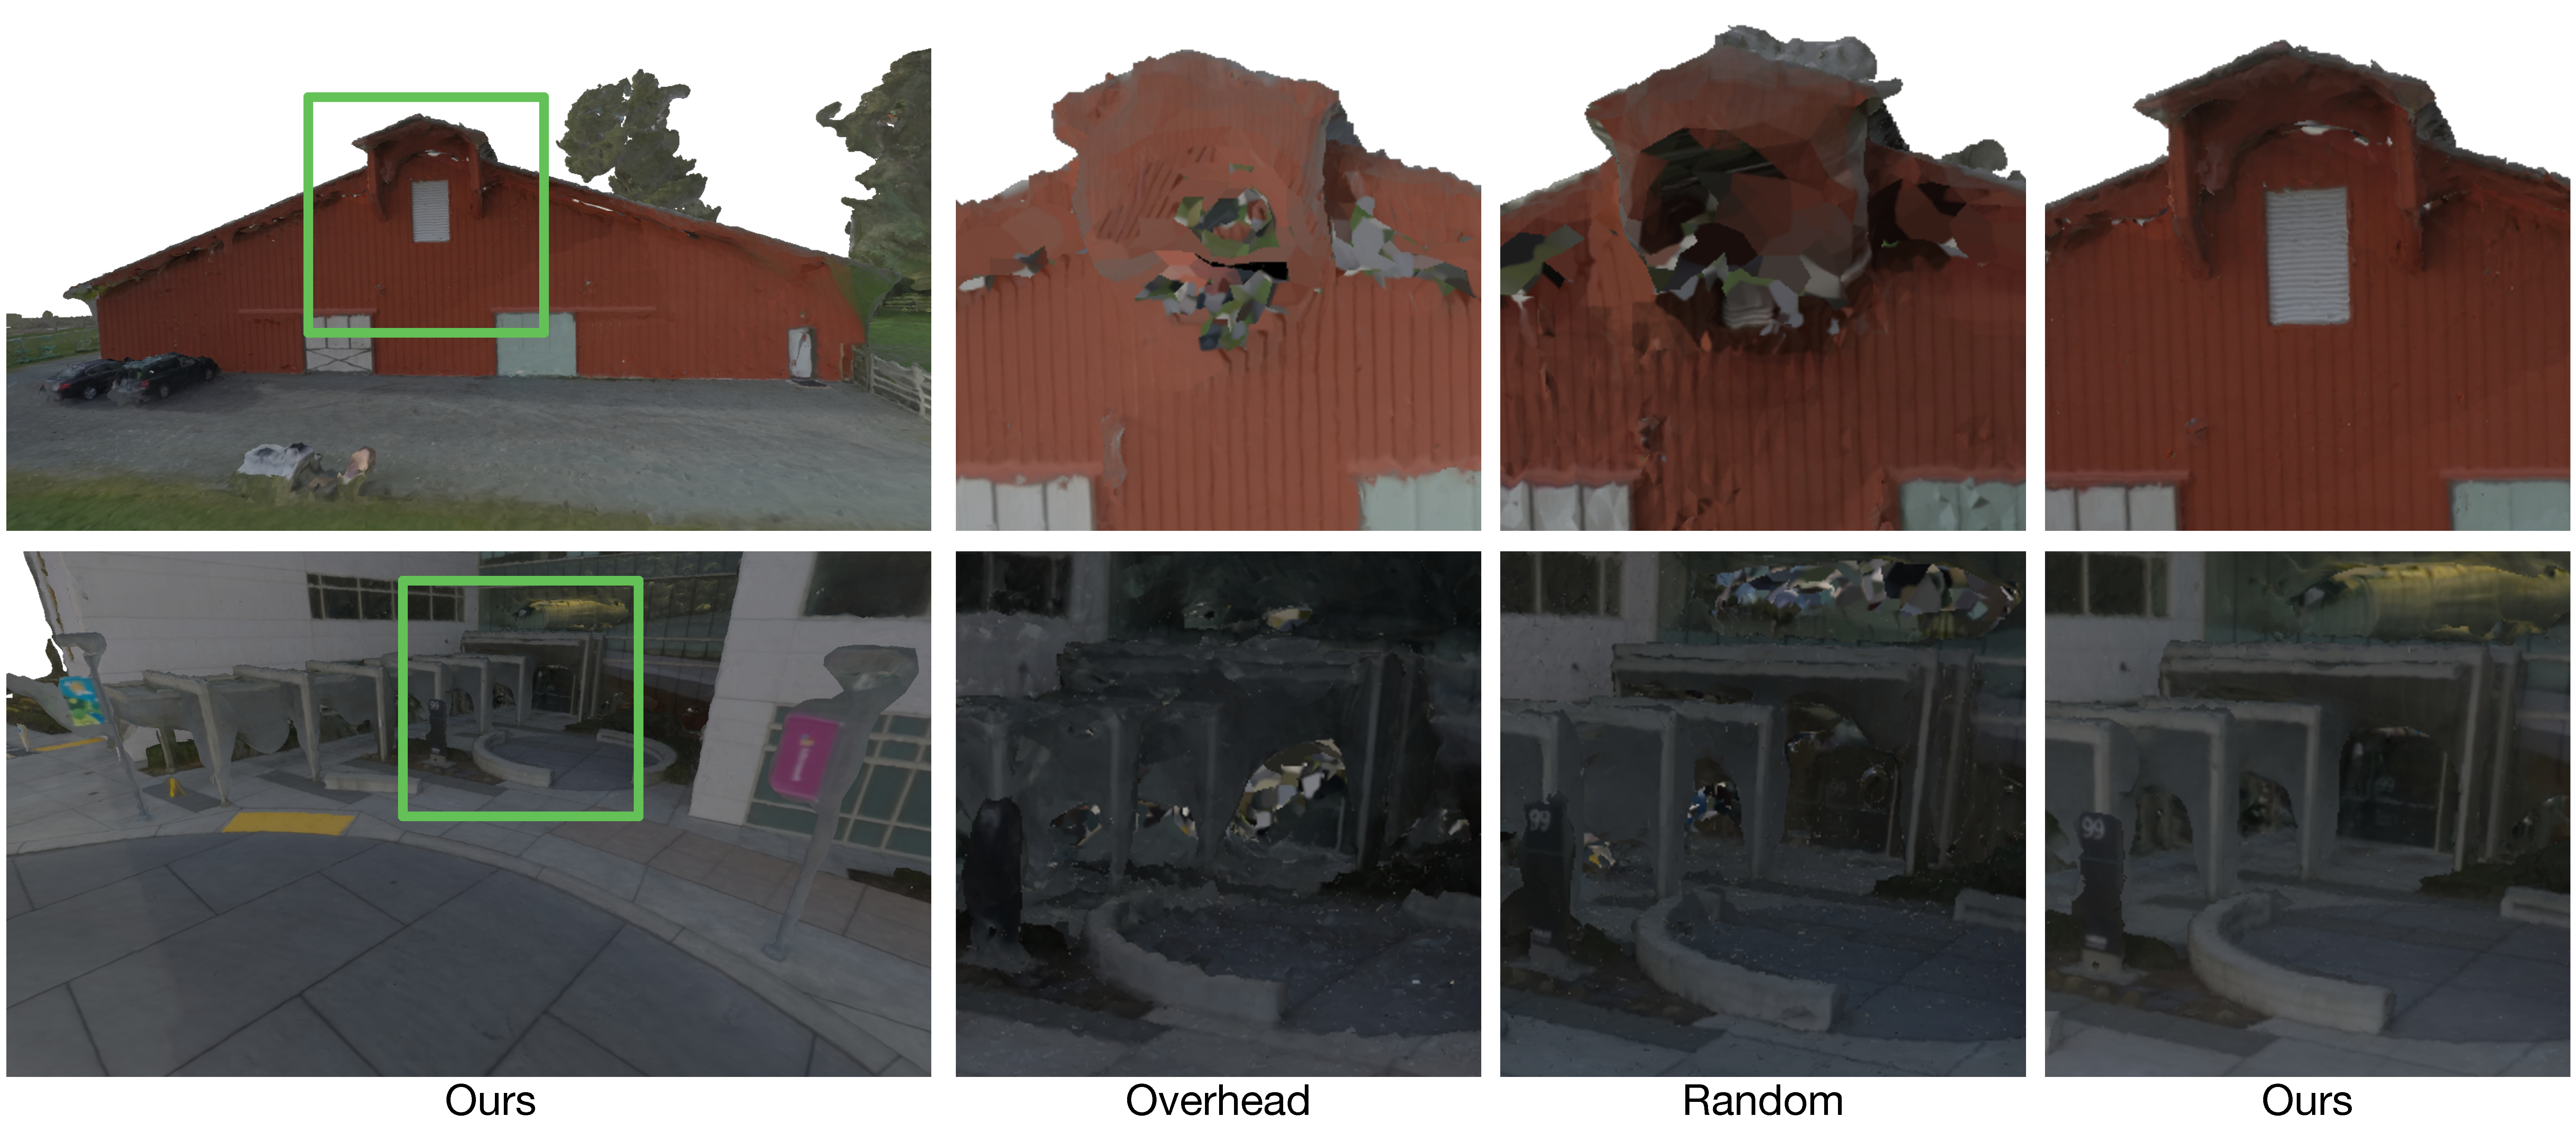
\includegraphics[width=0.98\textwidth]{images/2017_iccv/real_world_results.jpg}{\vspace{-7pt}}
\end{center}
\caption{
Qualitative comparison of the 3D reconstructions obtained from an overhead trajectory, a random trajectory, and our trajectory for two real-world scenes.
Our reconstructions contain noticeably fewer visual artifacts than the baseline reconstructions.
In all our experiments, we control for the flight time, battery consumption, number of images, and quality settings used in the 3D reconstruction.
\vspace{-2pt}
}
\label{fig:results_side_by_side}
\end{figure*}

\begin{figure*}[t]
\begin{center}
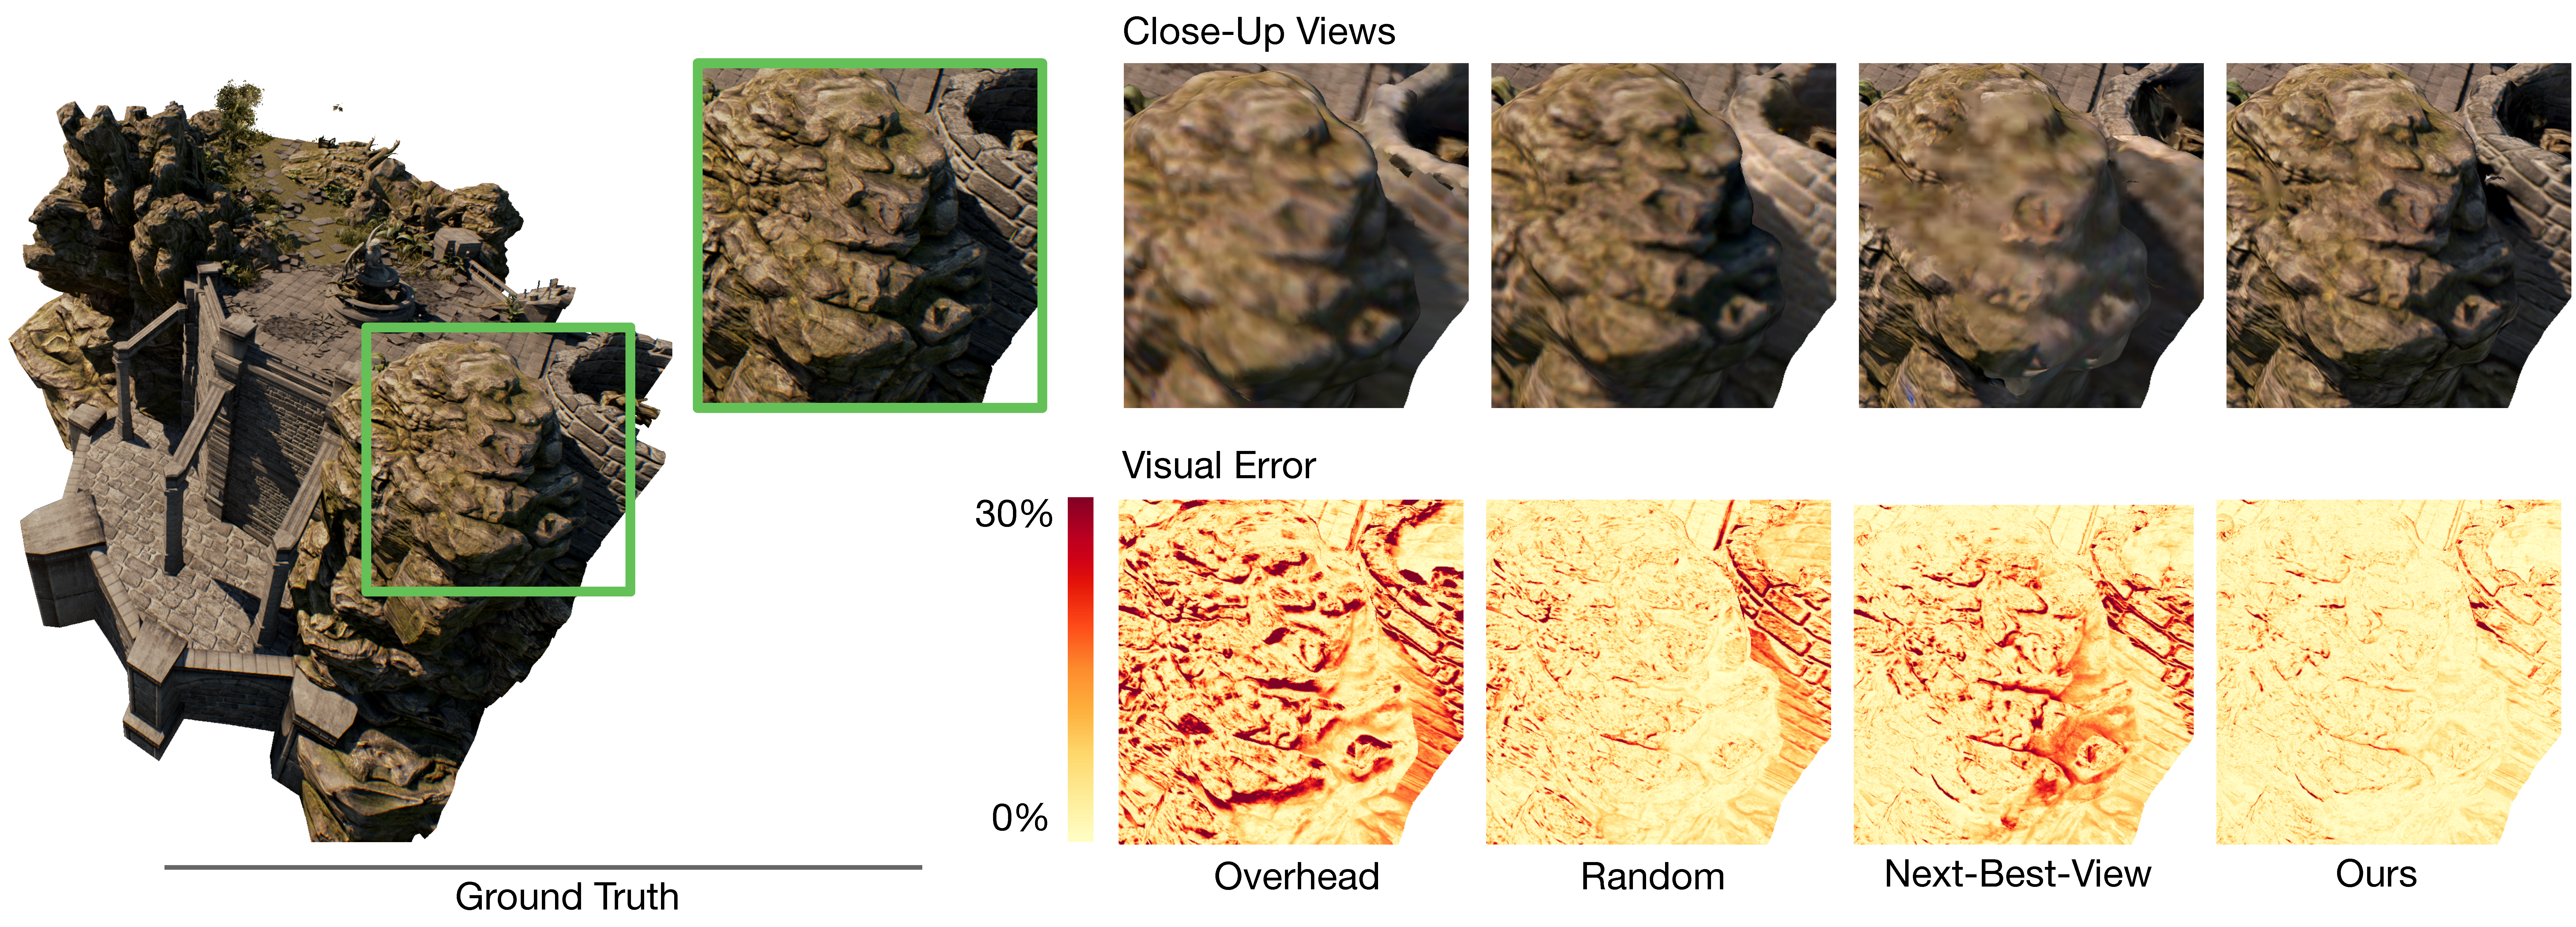
\includegraphics[width=0.98\textwidth]{images/2017_iccv/visual_error.jpg}{\vspace{-7pt}}
\end{center}
\caption{
Quantitative comparison of the 3D reconstructions obtained from an overhead trajectory, a random trajectory, a next-best-view trajectory, and our trajectory for our synthetic scene.
We show close-up renderings of each reconstruction, as well as per-pixel visual error, relative to a ground truth rendering of the scene.
Our method leads to quantitatively lower visual error than baseline methods.
\vspace{-12pt}
}
\label{fig:results_quantitative}
\end{figure*}

\vspace{-5pt}
\section{Evaluation}

\vspace{-1pt}
In all the experiments described in this section, we execute all drone flights at 2 meters per second, with a total travel budget of 960 meters (i.e., an 8 minute flight) unless otherwise noted.
All flights generate 1 image every 3.5 meters.
Each method has the same travel budget, and generates roughly 275 images.
Small variations in the number of generated images are possible, due to differences in how close each method gets to the travel budget.
We describe our drone hardware, data acquisition pipeline, and experimental methodology in more detail in the supplementary material.

\vspace{3pt}
\textbf{Real-World Reconstruction Performance}
We evaluated the real-world reconstruction performance of our algorithm by using it to scan three large outdoor scenes: a barn, an office building, and an industrial site.\footnote{We
conducted this experiment with an early implementation of our method that differs slightly from the implementation used in our other experiments.
In particular, the graph of camera positions used in this experiment included diagonal edges.
We subsequently excluded diagonal edges to enable our integer programming formulation to scale to larger problem instances. 
}
We show results from these experiments in Figures \ref{fig:teaser} and \ref{fig:results_side_by_side}, as well as in the supplementary material.
We compared our reconstruction results to two baseline methods: \textsc{Overhead} and \textsc{Random}.

\textsc{Overhead}.
We designed \textsc{Overhead} to generate trajectories that are representative of those produced by existing commercial flight planning software \cite{3dr:2017a,pix4d:2017a}.
\textsc{Overhead} generates a single flight at at a safe height above the scene; consisting of an orbit path that always points the camera at the center of the scene; followed by a lawnmower path that always points the camera straight down.

\textsc{Random}.
We designed \textsc{Random} to have roughly the same level of scene understanding as our algorithm, except that \textsc{Random} does not optimize our coverage function.
We gave \textsc{Random} access to the graph of camera positions generated by our algorithm, which had been pruned according to the free space in the scene.
\textsc{Random} generates trajectories by randomly selecting graph nodes to visit and traveling to them via shortest paths, until no more nodes can be visited due to the travel budget.
\textsc{Random} always points the camera towards the center of the scene, which is a reasonable strategy for the scenes we consider in this paper.

During our \emph{explore} phase, we generate an orbit trajectory exactly as we do for \textsc{Overhead}.
For the scenes we consider in this paper, this initial orbit trajectory is always less than 250 meters.

When generating 3D\ reconstructions, our algorithm and \textsc{Random} have access to the images from our \emph{explore} phase, but \textsc{Overhead} does not.
The images in our \emph{explore} phase are nearly identical to the orbit images from \textsc{Overhead}, and would therefore provide \textsc{Overhead} with negligible additional information, so all three methods are directly comparable.
We generated 3D reconstructions using the commercially available Pix4Dmapper Pro software \cite{pix4d:2017b}, configured with maximum quality settings.

\vspace{-1pt}
\textbf{Reconstruction Performance on a Synthetic Scene}
We evaluated our algorithm using a photorealistic video game simulator, which
enabled us to measure reconstruction performance relative to known ground truth geometry and appearance.
We show results from this experiment in Figure \ref{fig:results_quantitative} and Table \ref{tbl:quantitative}.

Our experimental design here is exactly as described previously, except we acquired images by programmatically maneuvering a virtual camera in the Unreal Engine \cite{epic:2017a}, using the UnrealCV Python library \cite{qiu:2016}.
We also included an additional baseline method, \textsc{Next-Best-View}, that greedily selects nodes according to their marginal submodular reward, and finds an efficient path to connect them using the Approx-TSP algorithm \cite{cormen:2009} until no more nodes can be added due to the travel budget.
This method is intended to be representative of the \emph{next-best-view} planning strategies that occur frequently in the literature \cite{fan:2016,hollinger:2013,krainin:2011,wu:2014}, including those that have been applied to aerial 3D scanning \cite{dunn:2009a,hoppe:2012,mostegel:2016,schmid:2012}.

We chose the \textsc{Grass Lands} environment \cite{epic:2017b} as our synthetic test scene because it is freely available, has photorealistic lighting and very detailed geometry, and depicts a large outdoor scene that would be well-suited for 3D scanning with a drone.

We evaluated geometric reconstruction quality by measuring \emph{accuracy} and \emph{completeness} relative to a ground truth point cloud \cite{aanaes:2016,knapitsch:2017}.
We obtained our ground truth point cloud by rendering reference depth images arranged on an inward-looking sphere around the scene, taking care to manually remove any depth images that were inside objects.
We also evaluated visual reconstruction quality by measuring \emph{per-pixel visual error}, relative to ground truth RGB images rendered from the same inward-looking sphere around the scene \cite{waechter:2017}.
When evaluating per-pixel visual error, we took care to only compare pixels that contain geometry from inside the scanning region-of-interest for our scene.

When evaluating geometric quality, we obtained point clouds for each method by running VisualSFM \cite{wu:2013,wu:2007,wu:2011b,wu:2011a}, followed by the Multi-View Environment \cite{fuhrmann:2015}, followed by Screened Poisson Surface Reconstruction \cite{kazhdan:2013}, and finally by uniformly sampling points on the reconstructed triangle mesh surface.
When evaluating visual quality, we obtained textured 3D models for each method using the surface texturing algorithm of Waechter et al.~\cite{waechter:2014}.

\begin{table}[t]
\centering
\footnotesize
\begin{tabular}{@{}llll@{}}
\toprule
Method         & Accuracy       & Completeness   & Visual     \\
               & Error (mm)     & Error (mm)     & Error (\%) \\
\midrule
Overhead       & 170.2          & 583.8          & 7.1  \\
Random         & 126.5          & 557.2          & 4.4 \\
Next-Best-View & 122.8          & 330.7          & 3.6 \\
\textbf{Ours}  & \textbf{115.2} & \textbf{323.3} & \textbf{3.3} \\
\bottomrule
\end{tabular}
\normalsize
\vspace{5pt}
\caption{
Quantitative comparison of the 3D reconstructions obtained from an overhead trajectory, a random trajectory, a next-best-view trajectory, and our trajectory for our synthetic scene.
For all the columns in this table, lower is better.
We report the mean per-pixel visual error across all of our test views, where 100\% per-pixel error corresponds to the $l_2$ norm of the difference between black and white in RGB space.
Our method quantitatively outperforms baseline methods, both geometrically (i.e., in terms of accuracy and completeness) and visually.
\vspace{-13pt}
}
\label{tbl:quantitative}
\end{table}

\begin{figure}[t]
\begin{center}
\includegraphics[width=0.40\textwidth]{images/2017_iccv/00_quantitative.pdf}{\vspace{-14pt}}
\end{center}
\caption{
Quantitative comparison of submodular orienteering algorithms on our synthetic scene.
(a) Submodular reward as a function of travel budget.
Our algorithm consistently obtains more reward than other algorithms.
%, across a range of different travel budgets.
All reconstruction results in this paper were produced with a budget of 960 meters (i.e., 8 minutes at 2 meters per second), shown with a grey dotted line.
For this budget, we obtain 20\% more reward than next-best-view planning. The p-SPIEL Orienteering algorithm \cite{singh:2009b} failed to consistently find a solution.
(b) Computation time as a function of travel budget.
On this plot, lower is better.
In terms of computation time, our algorithm is competitive with, but more expensive than, next-best-view planning.
We do not show computation times for the p-SPIEL Orienteering algorithm, because it took over 4 hours in all cases where it found a solution.\vspace{-6pt}
\vspace{-4pt}
}
\label{fig:results_orienteering}
\end{figure}

\vspace{3pt}
\textbf{Submodular Orienteering Performance}
\label{sec:submodperf}
We evaluated the submodular orienteering performance of our algorithm on our synthetic scene.
We performed this experiment after we have solved for the optimal camera orientation at every node in our graph, to facilitate the comparison of our algorithm to other submodular orienteering algorithms \cite{singh:2009b,zhang:2016}.
We show results from this experiment in Figure \ref{fig:results_orienteering}.

In this experiment, we included a baseline method that behaves identically to \textsc{Next-Best-View}, except it greedily selects nodes according to the ratio of marginal reward to marginal cost \cite{zhang:2016}.
We implemented all algorithms in Python, except for the p-SPIEL Orienteering algorithm \cite{singh:2009b}, where we used the MATLAB implementation provided by the authors.
We performed this experiment on a Mid 2015 Macbook Pro with a 2.8 GHz Intel Core i7 processor and 16GB of RAM.

%\begin{figure}[t]
%\begin{center}
%\includegraphics[width=0.47\textwidth]{figures/01_quantitative.pdf}
%\end{center}
%\caption{
%Comparing computation times of the Greedy and Lazy Greedy algorithms for submodular subset selection, for our real-world scenes.
%Smaller bars are better.
%For all our scenes, the Lazy Greedy algorithm is more than 450$\times$ faster than the Greedy algorithm, and achieves the same amount of submodular reward.
%}
%\label{fig:results_side_by_side}
%\end{figure}



\vspace{-5pt}
\section{Conclusions}
\vspace{-1pt}

We proposed an intuitive coverage model for aerial 3D scanning, and we made the observation that our model is submodular.
We leveraged submodularity to develop a computationally efficient method for generating scanning trajectories, that reasons jointly about coverage rewards and travel costs.
We evaluated our method by using it to scan three large real-world scenes, and a scene in a photorealistic video game simulator.
We found that our method results in quantitatively higher-quality 3D reconstructions than baseline methods, both geometrically and visually.

%Two optimality gaps are introduced in our method, where we first solve for the approximately optimal set of camera orientations, and subsequently solve for the approximately optimal path to an additive orienteering problem.
%Although we show strong empirical results against baseline methods, there is an opportunity to better understand the effects of these approximations in each stage of our method.

%There is also an opportunity to investigate other ways to model the usefulness of camera trajectories, that more faithfully capture the true 3D reconstruction process, while still being computationally tractable to optimize.

%An additional limitation is that our current implementation is strongly dependent on the validity of the initial geometry estimate; however, this is not fundamental constraint of our approach.

In the future, we believe trajectory optimization and geometric reasoning will enable drones to capture the physical world with unprecedented coverage and scale.
Individual drones may soon be able to execute very efficient scanning trajectories at the limits of their dynamics, and teams of drones may soon be able to execute scanning trajectories collectively and iteratively over very large scenes.

\vspace{-6pt}
\section*{Acknowledgements}
\vspace{-3pt}

We thank Jim Piavis and Ross Robinson for their expertise as our safety pilots;
Don Gillett for granting us permission to scan the barn scene;
3D Robotics for granting us permission to scan the industrial scene;
Weichao Qiu for his assistance with UnrealCV;
Jane E and Abe Davis for proofreading the paper;
and Okke Schrijvers for the helpful discussions.
This work began when Mike Roberts was a research intern at Microsoft Research, and was subsequently supported by a generous grant from Google.
%In the future, we believe the ideas in this paper could become part of the standard toolbox for aerial 3D scanning.
%By using our discrete scanning trajectories to initialize a continuous optimization method, it would be possible to generate smooth scanning trajectories that could be executed on drones at very high speeds.
%We are also optimistic that the trajectory optimization methods in this paper could be extended to coordinate teams of drones, leading to rapid scanning of very large scenes.

%We introduced a novel coverage model that characterizes the usefulness of a camera trajectory for multi-view stereo reconstruction, and we leveraged the submodularity property of our model to derive an algorithm for generating efficient scanning trajectories. We used our algorithm to scan three large outdoor scenes, and we evaluated our algorithm in a photorealistic simulator, where we obtained significantly higher-quality 3D reconstructions than a strong baseline method.

%In the future, we believe the ideas in this paper could become part of the standard toolbox for aerial 3D scanning. By using our discrete scanning trajectories to initialize a continuous optimization method, it would be possible to generate smooth scanning trajectories that could be executed on drones at very high speeds. Submodular trajectory optimization could also enable teams of drones to scan very large scenes (e.g., an entire university campus) fully autonomously, and with unprecedented geometric fidelity.

\section{Explore Phase: Estimating the Scene Geometry and Free Space}
\label{sec:free_space}

In this section, we describe our high-level strategy for data acquisition, as well as our multi-view stereo processing pipeline for estimating the scene geometry and free space.
Our goals in this section are twofold.
First, we would like to obtain a rough estimate of the scene geometry, in the form of a triangle mesh in real-world coordinates.
Second, we would like to obtain a strictly conservative estimate of the free space, in the form of an occupancy volume in real-world coordinates.
Together, these complimentary scene representations will enable us to plan trajectories that maximize the quality of a 3D reconstruction.

\vspace{-12pt}
\paragraph{Drone Camera Hardware}
Our system requires access to a drone camera that can be commanded to fly along pre-specified camera trajectories, given in GPS coordinates (i.e., latitude, longitude, altitude).
The drone camera must also take geotagged images of the scene at roughly constant intervals (e.g., one image every few meters).
We require geotagged images, in order to establish a correspondence between the physical world and the arbitrary coordinate system of our multi-view stereo reconstruction.
In our system, we use the 3D Robotics Solo drone \cite{3dr:2017b} equipped with a GoPro Hero 4 camera.

\vspace{-12pt}
\paragraph{User Input}
Our system requires two bounding boxes as input, each of which can easily be drawn by a user on a 2D map (e.g., Google Maps) and extruded vertically.
The first bounding box, $\mathbf{b}_s$, specifies the volume that the user wants to scan.
The second bounding box, $\mathbf{b}_c$, specifies the volume that the drone is allowed to fly within.
We require that $\mathbf{b}_c$ be made sufficiently tall, so that the entire ceiling of $\mathbf{b}_c$ is free of obstacles.
This requirement is necessary to give our drone some non-trivial region of free space that it can safely explore, prior to resolving any scene geometry.
We do not assume initially that any other space is free.

\vspace{-12pt}
\paragraph{Initial Camera Trajectory}
Our system begins by flying the drone in an elliptical orbit trajectory around the ceiling of $\mathbf{b}_c$, pointing the camera at the center of $\mathbf{b}_s$.
For the scenes we consider in this paper, this initial elliptical trajectory consumes roughly 25\% of our drone's travel budget.

\vspace{-12pt}
\paragraph{Dense Multi-View Stereo}
After we have flown an initial camera trajectory, the first step in our image processing pipeline is to run the structure-from-motion software VisualSFM \cite{wu:2013,wu:2007,wu:2011b,wu:2011a} on the sequence of images acquired by our drone.
Our next step is to run the depth map reconstruction step of the Multi-View Environment (MVE) \cite{fuhrmann:2015}.
In our implementation, we set the \emph{scale} parameter of MVE such that the reconstructed depth maps will be at a resolution of at least 512$\times$512 (e.g., if the images we originally capture are 2048$\times$2048, we set the \emph{scale} parameter to 2).
For the scenes we consider in this paper, computing structure-from-motion and dense multi-view stereo takes roughly 15 minutes, and is the dominant cost in our explore phase.

\vspace{-12pt}
\paragraph{Mapping Between Coordinate Systems}
We perform all our trajectory planning in real-world coordinates, using the UTM coordinate system \cite{usgs:2001}.
UTM coordinates are similar to GPS coordinates, in the sense that they describe positions on the surface of the Earth.
However, unlike GPS coordinates, the UTM coordinate axes are approximately orthogonal, and the default UTM units are meters.
Together, these properties make UTM coordinates well-suited for trajectory planning.

%However, it is convenient for a user to specify input bounding boxes in GPS coordinates (e.g., by drawing on a 2D map).
%Moreover, the communication interface to our drone requires that we specify trajectories in GPS coordinates.
%We use the utm Python library [???] to map back and forth between GPS and UTM coordinates.

In order to use our reconstructed scene geometry for trajectory planning, we must establish a correspondence between the UTM coordinate system and the arbitrary coordinate system of the reconstructed geometry.
We estimate this correspondence by considering our sequence of geotagged camera positions (in UTM coordinates), and the sequence of estimated camera positions recovered during our structure-from-motion step (in reconstruction coordinates).
We estimate the similarity transform that maps from reconstruction coordinates to UTM coordinates using standard numerical techniques \cite{sorkine:2017}.

\vspace{-12pt}
\paragraph{Obtaining an Oriented Point Cloud and Occupancy Volume}
We generate an oriented point cloud of the scene geometry, and an occupancy volume of the scene's free space, using our own modified version of MVE.
Given a collection of camera poses and corresponding depth images, we obtain our point cloud by projecting each depth image into reconstruction coordinates, and then into UTM coordinates.

We generate an occupancy volume of the free, occupied, and unknown space using a simple space carving algorithm.
For every depth observation in every depth image, we project the depth observation and corresponding camera into UTM coordinates.
This projection defines a ray that starts at the camera and ends at the depth observation.
In our occupancy volume, we mark every interior voxel along this ray as being free, and we mark the last voxel along this ray as being occupied.
After having generated our occupancy volume in this way, we create an extra safety buffer around obstacles by dilating the occupied space by 4 meters in every direction.
This safety buffer is conservative, in the sense that it is roughly twice the diameter of the largest localization errors we observed on our drone hardware during field testing.
We consider all unmarked voxels to be unknown.
We store our occupancy volume efficiently in an OctoMap data structure \cite{hornung:2013}.

After this space carving step is complete, we assume that our occupancy volume strictly underestimates the free space in the scene.
This assumption is justified by the following three observations.
First, MVE\ aggressively filters outlier depth observations. So, although MVE does not produce a depth observation at every pixel of every depth image, the observations that MVE does produce tend to be very reliable.
Second, we only mark a voxel as being free if there is explicit evidence for doing so (i.e., there is some camera in front of it, that has observed some surface point behind it).
Third, we create a large safety buffer around all observed surfaces, to account for any small errors in the MVE depth images.

\vspace{-12pt}
\paragraph{Surface Reconstruction}
Given an oriented point cloud of our scene geometry in UTM coordinates, we obtain a water-tight triangle mesh surface by running the Screened Poisson Surface Reconstruction algorithm \cite{kazhdan:2013} on the point cloud.
In our implementation, we set the \emph{depth} parameter of Screened Poisson Surface Reconstruction to 7, which produces a coarse triangle mesh quickly.
To maximize the effective resolution of our surface reconstruction, we clip the input point cloud against the user-specified bounding box $\mathbf{b}_s$.
As a post-processing step, we apply the \emph{surface trimming} tool implemented in the Screened Poisson Surface Reconstruction codebase with a \emph{trim} parameter of 7, and we use MeshLab \cite{cignoni:2008} to remove isolated triangle mesh connected components with fewer than 2000 faces.
At this point in our pipeline, we have a triangle mesh representation of the scene geometry, as well as an occupancy volume representation of the scene's free space, both in UTM coordinates.

\begin{table}[t]
\centering
\footnotesize
\begin{tabular}{@{}lllll@{}}
\toprule
Scene           & Extent of              & Extent of              & Grid    & Number of  \\
                & $\mathbf{b}_s$ (m)     & $\mathbf{b}_c$ (m)     & Spacing & Grid Nodes \\
                &                        &                        & (m)     & \\
\midrule
Barn            & 34$\times$24$\times$28 & 44$\times$29$\times$58 & 4.0     & 1440 \\
Office Building & 40$\times$25$\times$37 & 50$\times$30$\times$47 & 3.5     & 1890 \\
Industrial Site & 34$\times$25$\times$31 & 54$\times$30$\times$51 & 4.0     & 1456 \\
Grass Lands     & 48$\times$30$\times$41 & 78$\times$45$\times$71 & 4.5     & 2880 \\
\bottomrule
\end{tabular}
\normalsize
\vspace{5pt}
\caption{
Grid spacing parameters for each of our scenes.
}
\vspace{-5pt}
\label{tbl:grid}
\end{table}

\vspace{-12pt}
\paragraph{Sampling Details}
We uniformly sample points on our reconstructed surface using the Poisson Disk Sampling technique \cite{corsini:2012} implemented in MeshLab \cite{cignoni:2008}.
In our implementation, we request that MeshLab return 1500 surface samples.
MeshLab is not guaranteed to return exactly this many surface samples, and in practice returns roughly 2000 surface samples.

In our implementation, we sample camera positions in the bounding box $\mathbf{b}_c$ by constructing a uniform grid with a grid spacing that that we specify per scene, ranging from 3.5 to 4.5 meters per grid node.
If our specified grid spacing does not align exactly with the borders of $\mathbf{b}_c$, we independently adjust the grid spacing along each axis to be slightly more dense, so as to align with exactly with the borders of $\mathbf{b}_c$.
For the scenes we consider in this paper, this range of grid densities leads to grids containing between 1440 and 2880 grid nodes.
We choose our grid spacing to strike a balance between being as dense as possible, while also not leading to too many integer variables in our integer programming formulation. We include the exact grid spacing parameters for each of our scenes in Table \ref{tbl:grid}.

We sample camera orientations by generating uniformly spaced samples on a downward-facing hemisphere.
In our implementation, we generate 50 uniformly spaced samples using standard numerical techniques \cite{devert:2012}.

\vspace{-0pt}
\section{Efficiently Evaluating Coverage}
\label{sec:evaluating_coverage}

In this section, we demonstrate how to evaluate coverage efficiently for an arbitrary subset of cameras. 
It is important that we can evaluate coverage efficiently, because we must evaluate it many times, for many different subsets, in our algorithm for generating scanning trajectories.
Our strategy will be to apply a discrete Monte Carlo approximation of coverage that we can evaluate using matrix operations. 

\vspace{-12pt}
\paragraph{Evaluating Coverage using Matrix Operations}
It is not immediately obvious how to evaluate our coverage model efficiently, due to the unpleasant irregular integration domain in equation (1) in the main paper.
Our approach begins by replacing this irregular domain with a regular domain, using an indicator function representation to mask out the covered region $V_j$,
%
\begin{equation}
\begin{aligned}
f(C) = \sum_{j=0}^{J} \int_{H_j} w_j(\mathbf{h}) v_{j}(\mathbf{h}) d\mathbf{h}
\end{aligned}
\end{equation}
%
where the notation $\int_{H_j} d\mathbf{h}$ refers to a surface integral over the entire hemisphere $H_j$;
and $v_j(\mathbf{h})$ is an indicator function that equals 1 when the hemisphere location $\mathbf{h}$ is in the covered region $V_j$, and equals 0 otherwise.
Next, we approximate our regular hemispherical integral with a discrete Monte Carlo approximation,
%
\begin{equation}
\begin{aligned}
F(C)= \sum_{j=0}^{J} 2\pi \frac{1}{K} \sum_{k=1}^{K} w_j(\mathbf{h}_k) v_{j}(\mathbf{h}_k)
\end{aligned}
\end{equation}
%
where
$F(C) \approx f(C)$ is the discrete approximation of our coverage function;
the constant $2 \pi$ arises because we are integrating over the hemisphere;
$K$ is the number of discrete samples on the hemisphere;
and $k$ is an index that refers to the discrete hemisphere sample location $\mathbf{h}_k$.
In this form, it becomes clear that we can represent our discrete coverage model with the following dot product,
%
\begin{equation}
\begin{aligned}
F(C) = \mathbf{w}^T \mathbf{v}
\end{aligned}
\end{equation}
%
where $\mathbf{w}$ is the stacked vector of all our (normalized) weight function values $2 \pi \frac{1}{K}w_j(\mathbf{h}_k)$;
and $\mathbf{v}$ is the stacked vector of all our coverage indicator function values $v_j(\mathbf{h}_k)$.
We refer to $\mathbf{v}$ as a \emph{coverage indicator vector}.
In our implementation, we set $K=256$, and we generate our hemisphere sample locations $\mathbf{h}_k$ using standard numerical techniques \cite{devert:2012}.


\begin{figure}[t]
\begin{center}
\includegraphics[width=0.47\textwidth]{images/2017_iccv_supplementary/coverage_matrix.pdf}{\vspace{-7pt}}
\end{center}
\caption{
Our matrix representation for efficiently evaluating coverage, for arbitrary subsets of cameras.
We begin by pre-computing a coverage indicator matrix that represents the independent contribution of each camera to the total coverage.
We recover the coverage indicator vector  for a particular subset of cameras by selecting the appropriate subset of columns from our matrix, and performing a logical \textsc{or} operation across the rows of the resulting matrix.
We evaluate our coverage model for this subset of cameras by multiplying the coverage indicator vector with a weight vector.
We use this efficient matrix representation to evaluate coverage for many different subsets of cameras, in our algorithm for generating scanning trajectories.
\vspace{-5pt}
}
\label{fig:coverage_matrix}
\end{figure}

\vspace{-12pt}
\paragraph{Evaluating Coverage for any Subset of Cameras}
In the previous subsection, we showed how to evaluate our coverage model efficiently for a particular set of cameras.
In order to optimize our model, we will need to efficiently evaluate coverage for many different subsets of cameras.
In other words, we would like to efficiently evaluate the following expression, 
%
\begin{equation}
\begin{aligned}
F(C_S) = \mathbf{w}^T \mathbf{v}_S
\end{aligned}
\end{equation}
%
where $C_S \subseteq C$ is an arbitrary subset of cameras;
and $\mathbf{v}_S$ is the coverage indicator vector for the cameras in $C_S$. 

We can efficiently evaluate our model for any subset of cameras $C_S \subseteq C$ by pre-computing a \emph{coverage indicator matrix}, $\mathbf{D}$ (see Figure \ref{fig:coverage_matrix}).
Intuitively speaking, we define the matrix $\mathbf{D}$ to represent the independent contribution of each camera to the total coverage.
Each row of $\mathbf{D}$ corresponds to a particular sampling location on a particular hemisphere.
Each column of $\mathbf{D}$ corresponds to a particular camera in $C$.
Stating our definition of $\mathbf{D}$ more precisely, we set the entry of $\mathbf{D}$ corresponding to \textbraceleft hemisphere $H_j$, hemisphere location $\mathbf{h}_k$, camera $\mathbf{c}_i$\textbraceright ~equal to 1 if \textbraceleft hemisphere $H_j$, hemisphere location $\mathbf{h}_k$\textbraceright ~is covered by the disk $D^j_i$, and equal to 0 otherwise.


\vspace{-5pt}
\section{Designing the Parameters of Our Coverage Model}
\label{sec:evaluating_coverage}

In this section, we provide the exact parameters we use in our coverage model.
In our implementation, we set the radius of each disk $D^j_i$ to decay exponentially as a camera moves away from a surface point.
We chose an exponential decay model as a matter of convenience, because it was intuitive for us to specify disk size in terms of a decay half-life.
When a surface point is not visible from a camera, we define the corresponding disk to have zero radius.
We determine visibility by raycasting against our coarse triangle mesh estimate of the scene geometry.

Stating our model more precisely, we define each disk as the intersection of a hollow unit sphere, centered at the surface point; and a solid cone that has its apex at the surface point, and is oriented towards the camera.
We control the solid angle of each disk by controlling the apex angle of this cone.
We define the apex \emph{half angle} $\theta^j_i$ of each cone in radians as follows,
%
\begin{equation}
\begin{aligned}
\theta^j_i = \theta_\text{max} 2^{ \frac{ -\max(t^j_i - t_0, 0) }{ t_{\text{half}} } }
\end{aligned}
\end{equation}
%
where
$\theta_{\text{max}}$ is the largest possible apex half angle in radians;
$t_0$ is the distance in meters from a camera to a surface point, beyond which our half angle doesn't get any larger;
$t_{\text{half}}$ is the decay half-life of the our half angle in meters; and
$t^j_i$ is the distance from camera $\mathbf{c}_i$ to surface point $\mathbf{s}_j$ in meters.
In our implementation, we set $\theta_{\text{max}} = \frac{1}{2} \frac{\pi}{180} 45$ radians, $t_0 = 4$ meters, and $t_\text{half} = 12$ meters.

In our implementation, we set each weight function $w_j(\mathbf{h})$ to have a cosine-weighted falloff as follows,  
%
\begin{equation}
\begin{aligned}
w_j(\mathbf{h}) = \cos \alpha_\mathbf{h}
\end{aligned}
\end{equation}
%
where $\alpha_\mathbf{h}$ is the angle formed by the hemisphere pole and the vector from the hemisphere origin to the hemisphere location $\mathbf{h}$.



\begin{Listing}[t]
\caption{
The greedy algorithm for maximizing a monotone submodular function, subject to a cardinality constraint and a mutual exclusion constraint.
Evaluating the $\argmax$ expression on line 4 requires evaluating $f$ once for each element in the set $G$, leading to many function evaluations. 
}
\label{lst:greedy}

\begin{algorithmic}[1]

\small

\REQUIRE { ~~\\ \vspace{-7pt}
\begin{itemize}
\item A ground set of elements $C$. \vspace{-7pt}
\item A monotone submodular function $f(C_{S})$ to be maximized, where $C_S \subseteq C$. \vspace{-7pt}
\item A cardinality constraint $|C_{S}| = N$. \vspace{-7pt}
\item A mutual exclusion constraint $C_{S} \in \mathcal{M}$, that defines which elements in $C$ are incompatible.
\end{itemize}
}

\ENSURE  { ~\\ \vspace{-7pt}
\begin{itemize}
\item A subset $C_{S} \subseteq C$ that maximizes $f$ to within 50\% of global optimality, subject to the cardinality constraint and mutual exclusion constraint. \vspace{-12pt}
\end{itemize}
~}

\STATE { $ S \gets \varnothing $ }
\STATE { $ G \gets C $ }

\FOR { $ i \gets 0 \text{ to } N $ }

    \STATE { $ g^{\star} \gets \argmax_{g \in G} f(S \cup g) - f(S) $ }
    \STATE { $ I         \gets \text{all the elements in } G \text{ that are incompatible with } g^{\star} $ }
    \STATE { $ S         \gets S \cup g^{\star} $ }
    \STATE { $ G         \gets G ~\backslash~ \{ I, g^{\star} \} $ }
    
\ENDFOR

\STATE { $ C_S \gets S $ }

\end{algorithmic}
\end{Listing}



\begin{Listing}[t]
\caption{
The lazy greedy algorithm for maximizing a monotone submodular function, subject to a cardinality constraint and a mutual exclusion constraint.
This algorithm maintains a lazily updated list of marginal rewards, $m_g$.
When a marginal reward in this list is stale (i.e., when $u_g = \text{False}$), the value $m_g$ can be interpreted as an upper bound on the true marginal reward, due to submodularity.
This observation can be used to skip a large number of function evaluations.
The lazy greedy algorithm drastically reduces the number of times $f$ must be evaluated, as compared to the greedy algorithm.
}
\label{lst:lazy_greedy}

\begin{algorithmic}[1]

\small

\REQUIRE { ~~\\ \vspace{-7pt}
\begin{itemize}
\item A ground set of elements $C$. \vspace{-7pt}
\item A monotone submodular function $f(C_S)$ to be maximized, where $C_S \subseteq C$. \vspace{-7pt}
\item A cardinality constraint $|C_S| = N$. \vspace{-7pt}
\item A mutual exclusion constraint $C_S \in \mathcal{M}$, that defines which elements in $C$ are incompatible.
\end{itemize}
}

\ENSURE  { ~\\ \vspace{-7pt}
\begin{itemize}
\item A subset $C_S \subseteq C$ that maximizes $f$ to within 50\% of global optimality, subject to the cardinality constraint and mutual exclusion constraint. \vspace{-12pt}
\end{itemize}
~}

\STATE { $ S \gets \varnothing $ }
\STATE { $ G \gets C $ }

\FORALL { $ g \in G $ }

    \STATE { $ m_g \gets f(S \cup g) - f(S) $ }
    \STATE { $ u_g \gets \text{True} $ }

\ENDFOR

\FOR { $i \gets 0 \text{ to } N$ }

    \STATE { $ g^{\star} \gets \argmax_{g \in G} m_g $ }

    \WHILE { $ \text{not } u_{g^{\star}} $ }

        \STATE { $ m_{g^{\star}} \gets f(S \cup g^{\star}) - f(S)$ }
        \STATE { $ u_{g^{\star}} \gets \text{True}$ }
        \STATE { $ g^{\star}     \gets \argmax_{g \in G} m_g $ }

    \ENDWHILE

    \STATE { $ I \gets \text{all the elements in } G \text{ that are incompatible with } g^{\star} $ }
    \STATE { $ S \gets S \cup g^{\star} $ }
    \STATE { $ G \gets G ~\backslash~ \{ I, g^{\star} \} $ }

    \FORALL { $ g \in G $ }

        \STATE { $ u_g \gets \text{False} $ }
    
    \ENDFOR

\ENDFOR

\STATE { $ C_S \gets S $ }

\end{algorithmic}
\end{Listing}

\vspace{-0pt}
\section{The Greedy Algorithm for Maximizing Submodular Functions}
\label{sec:greedy}

In this section, we provide additional details regarding the greedy algorithm for maximizing submodular functions.
The problem in equation (2) in the main paper can be solved to within 50\% of global optimality with the greedy algorithm in Listing \ref{lst:greedy}.
To see that this is the case, we first make the observation that our coverage model is \emph{monotone} (i.e., selecting more camera poses never reduces our coverage score) \cite{krause:2014}.
We also make the observation that our mutual exclusion constraint is an instance of a more general mathematical object known as a \emph{partition matroid constraint} \cite{krause:2014}.
It is known that maximizing a monotone submodular function, subject to a cardinality constraint and a partition matroid constraint, can be solved to within 50\% of global optimality with the greedy algorithm \cite{krause:2014}.

The greedy algorithm can be expensive to run on large problems, because it must evaluate the submodular function many times (Listing \ref{lst:greedy}, line 4).
Indeed, the greedy algorithm takes several hours to run on the problem instances we consider in this paper. 
Fortunately, we can leverage submodularity to avoid a very large fraction of this computational effort.
The main insight in this approach, is that the marginal reward for adding an element only ever decreases as more elements are added to the greedy solution, due to submodularity.
Therefore, we can maintain a priority queue of marginal rewards, and we can \emph{lazily} update this queue.
When a marginal reward in our queue is stale, it can be interpreted as an upper bound on the true marginal reward. 
This insight can be used to safely skip a large fraction of function evaluations, in an approach known as the \emph{lazy greedy} algorithm \cite{krause:2014}.
We provide pseudocode for the lazy greedy algorithm, including the necessary modifications to handle our mutual exclusion constraint, in Listing \ref{lst:lazy_greedy}.
For the problem instances we consider in this paper, the lazy greedy algorithm reduces computation time by several orders of magnitude.

\vspace{0pt}
\section{Detailed Formulation of Orienteering as an Integer Linear Program}

In this section, we transform the orienteering problem in equation (4) in the main paper, into a standard integer linear program.
In this derivation, we follow the formulation of Letchford et al.~\cite{letchford:2013}.
However, we express the objective and constraints from this formulation in matrix form, which makes the problem easier to express in a high-level modeling language (e.g., CVXPY \cite{cvxpy:2016}).

We begin by replacing each undirected edge in our graph with two directed \emph{arcs}, each with the same cost as the original undirected edge.
We use the term arc to refer to a directed edge in our modified graph.
We define the indicator vector $\mathbf{x}$ to represent whether or not each arc is traversed.
We define the indicator vector $\mathbf{y}$ to represent whether or not each node in our graph is visited.
We define the vector $\mathbf{g}$ to contain the cumulative costs incurred so far, when beginning to traverse each arc.
Finally, we define the constant vector $\mathbf{f}$ to contain the additive reward at each each node, and we define the constant vector $\mathbf{r}$ to contain the instantaneous cost of traversing each arc.

To help coordinate our optimization problem, we also define inbound and outbound \emph{node-arc indicator matrices}, $\mathbf{A}^{\text{in}}$ and $\mathbf{A}^{\text{out}}$ respectively.
The rows of these matrices represent the nodes in our graph, and columns represent the arcs.
We set the entry of $\mathbf{A}^{\text{in}}$ corresponding to \{node $n$, arc $m$\} equal to 1 if arc $m$ is an inbound arc for node $n$, and equal to 0 otherwise. 
We define $\mathbf{A}^{\text{out}}$ similarly, but with respect to the outbound arcs.
We use the notation $\mathbf{A}_{R}$ to refer to the row of $\mathbf{A}$ corresponding to the root node (i.e., the node where our path must start and end), and we use the notation $\mathbf{A}_{R'}$ to refer to all the other rows of $\mathbf{A}$.


With this notation in place, we define our integer linear program as follows,
%
\begin{subequations}
\label{eqn:ilp}
\begin{equation}
\begin{aligned}
\mathbf{x}^{\star}, \mathbf{y}^{\star}, \mathbf{g}^{\star} = \argmax_{ \mathbf{x}, \mathbf{y}, \mathbf{g} } \mathbf{f}^T \mathbf{y}
\end{aligned}
\label{eqn:ilp_a}
\end{equation}
%
\vspace{-5pt}
%
\begin{equation}
\begin{aligned}
\text{subject to} ~~~~~ \mathbf{r}^T \mathbf{x} \leq B
\end{aligned}
\label{eqn:ilp_b}
\end{equation}
%
\vspace{-5pt}
%
\begin{equation}
\begin{aligned}
\mathbf{A}^{\text{out}}_{R}  \mathbf{x} & \geq \mathbf{1}             &     \mathbf{A}^{\text{out}}      \mathbf{x}                                          & = \mathbf{A}^{\text{in}}      \mathbf{x} \\
\mathbf{A}^{\text{out}}_{R'} \mathbf{x} & \geq \mathbf{y}_{R'} ~~~~~~ &     \mathbf{A}^{\text{out}}_{R'} \mathbf{g} - \mathbf{A}^{\text{in}}_{R'} \mathbf{g} & = \mathbf{A}^{\text{in}}_{R'} \mathbf{T} \mathbf{x} \\
\end{aligned}
\label{eqn:ilp_c}
\end{equation}
%
\vspace{-4pt}
%
\begin{equation}
\begin{aligned}
0 \leq \mathbf{g} \leq \mathbf{U} \mathbf{x}\\
\end{aligned}
\label{eqn:ilp_d}
\end{equation}
%
\vspace{-10pt}
%
\begin{equation}
\begin{aligned}
\mathbf{x} \in \{0,1\}^M ~~~~~ \mathbf{y} \in \{0,1\}^N ~~~~~ \mathbf{g} \in \mathbf{R}_{+}^M
\end{aligned}
\label{eqn:ilp_e}
\end{equation}
\end{subequations}
%
where
the matrix $\mathbf{T} = \mathbf{diag}( \mathbf{r} )$ helps us to calculate an intermediate matrix of instantaneous costs for inbound arcs;
the matrix $\mathbf{U} = \mathbf{diag}( \mathbf{1}B - \mathbf{r} )$ helps us to define the upper bounds for our cumulative cost variable $\mathbf{g}$;
and $M$ is the number of arcs in our graph and $N$ is the number of nodes. 
In this formulation, $\mathbf{x}$, $\mathbf{y}$, and $\mathbf{g}$ are decision variables, everything else is problem data.
Letchford et al.~refer to this integer linear program as a \emph{single-commodity flow} formulation for the orienteering problem \cite{letchford:2013}.

The objective in this optimization problem (\ref{eqn:ilp_a}) attempts to maximize the reward we collect, by activating as many nodes as possible.
The constraint in (\ref{eqn:ilp_b}) enforces our maximum budget on total path length.
The constraints in (\ref{eqn:ilp_c}) specify that: at least one of the outbound arcs for the root node must be active; the number of active outbound arcs must match the number of active inbound arcs at each node; if an outbound arc is active, then the node at its tail must be active; and the difference in cumulative cost at an outbound arc and a corresponding inbound arc, must match the instantaneous cost of the inbound arc.
The constraint in (\ref{eqn:ilp_d}) enforces that the cumulative costs incurred so far are less than the total budget.
Finally, the constraints in (\ref{eqn:ilp_e}) specify that $\mathbf{x}$ and $\mathbf{y}$ are Boolean indicator vectors, and that $\mathbf{g}$ is non-negative and real-valued.

The problem in equation (\ref{eqn:ilp}) is expressed in a standard form that can be given directly to an off-the-shelf solver.
Given a solution to the problem in equation (\ref{eqn:ilp}), we recover the sequence of visited nodes by following outbound arcs from the root until there are no more nodes to visit.
For each visited node, we look up its corresponding camera pose in our coarsened ground set to obtain a sequence of camera poses.

\vspace{-2pt}
\section{Evaluation Details}

In this section, we provide additional real-world reconstruction results, as well as additional methodological details for our synthetic scene experiments.

\vspace{-12pt}
\paragraph{Real-World Reconstruction Results}
We provide high-resolution renderings of our real-world reconstructions in Figure \ref{fig:results_supplementary}.

\vspace{-12pt}
\paragraph{Methodological Details for our Synthetic Scene Experiments}
When acquiring images for each method, we configured UnrealCV \cite{qiu:2016} to produce RGB images at a resolution of 512$\times$512.

When generating high-resolution reconstructions, we set the \emph{scale} parameter of MVE \cite{fuhrmann:2015} to 0.
We set the \emph{depth} parameter of the Screened Poisson Surface Reconstruction algorithm \cite{kazhdan:2013} to 9, which produces a detailed triangle mesh without overfitting to high-frequency noise in the point clouds estimated by MVE.
As in our explore phase, we clipped the input point cloud against the bounding box $\mathbf{b}_s$.
As a post-processing step, we applied the \emph{surface trimming} tool implemented in the Screened Poisson Surface Reconstruction codebase with a \emph{trim} parameter of 7, and we used MeshLab \cite{cignoni:2008} to remove isolated triangle mesh connected components with fewer than than 50000 faces.
We used the \emph{Gaussian damping} option when running the surface texturing algorithm of Waechter et al.~\cite{waechter:2014}.

When collecting ground truth data, we configured UnrealCV to produce RGB and depth images at a resolution of 2048$\times$2048.
We generated 256 uniformly distributed views on an inward-looking sphere around our scene using standard numerical techniques \cite{devert:2012}.
We set the center of our sphere to be the center of the bounding box $\mathbf{b}_s$, and we set its diameter to be 1.5$\times$ the maximum dimension of $\mathbf{b}_s$, which in our case was 72 meters.
We took care to manually remove images from our set of ground truth views that were inside objects.

When measuring geometric accuracy and completeness, we subsampled our ground truth point cloud to obtain a uniformly sampled point cloud, using the \emph{spatial subsampling} method implemented in CloudCompare \cite{cloudcompare:2017}.
When performing this subsampling operation, we set the minimum space between points to the 95$^{\text{th}}$ percentile of the distribution of nearest-neighbor distances in the original ground truth point cloud, which in our case was 0.0133 meters (i.e., prior to subsampling, 95\% of nearest-neighbor distances in the original ground truth point cloud were less than 0.0133 meters).
We sampled points on each reconstructed triangle mesh using the \emph{mesh sampling} method implemented in CloudCompare \cite{cloudcompare:2017}, where we set the desired sampling density to be $\frac{1}{0.0133^2} = 5653.2308$ points per square meter.

When measuring per-pixel visual error, we departed slightly from the formulation suggested by Waechter et al.~\cite{waechter:2017}.
Waechter et al.~suggest measuring visual error by computing zero-mean normalized cross-correlation (NCC) over small patches, so as to be robust to low-frequency discrepancies in illumination between the ground truth images and the test images (i.e., the images of a reconstructed 3D model).
In our synthetic scene, illumination is controlled perfectly, so we do not need this additional robustness.
Moreover, we found that NCC did not successfully localize the noticeable texturing artifacts on baseline reconstructed 3D\ models (e.g., the texturing artifacts visible in Figure 5 in the main paper).
For these reasons, we computed per-pixel differences in RGB space, instead of computing NCC.

Because we rendered ground truth views using UnrealCV, we needed to map the reconstructed 3D models into Unreal coordinates before rendering them and comparing them to the ground truth views.
In practice, our procedure for mapping into Unreal coordinates (see Section \ref{sec:free_space}) is accurate to within a few pixels, but is not perfect.
To prevent our visual quality metric from being dominated by very small coordinate system alignment errors, we computed per-pixel differences in the following way.
For each ground truth pixel location $\mathbf{z}$, we computed the difference between the ground truth image at $\mathbf{z}$, and each pixel in a 9$\times$9 patch centered at $\mathbf{z}$ in the test image.
We took the minimum difference over this patch as the per-pixel difference at $\mathbf{z}$.
In our experience, this approach provided a good balance between being robust to small alignment errors, while also effectively localizing noticeable texturing artifacts in the reconstructed 3D models.

\begin{figure*}[t]
\begin{center}
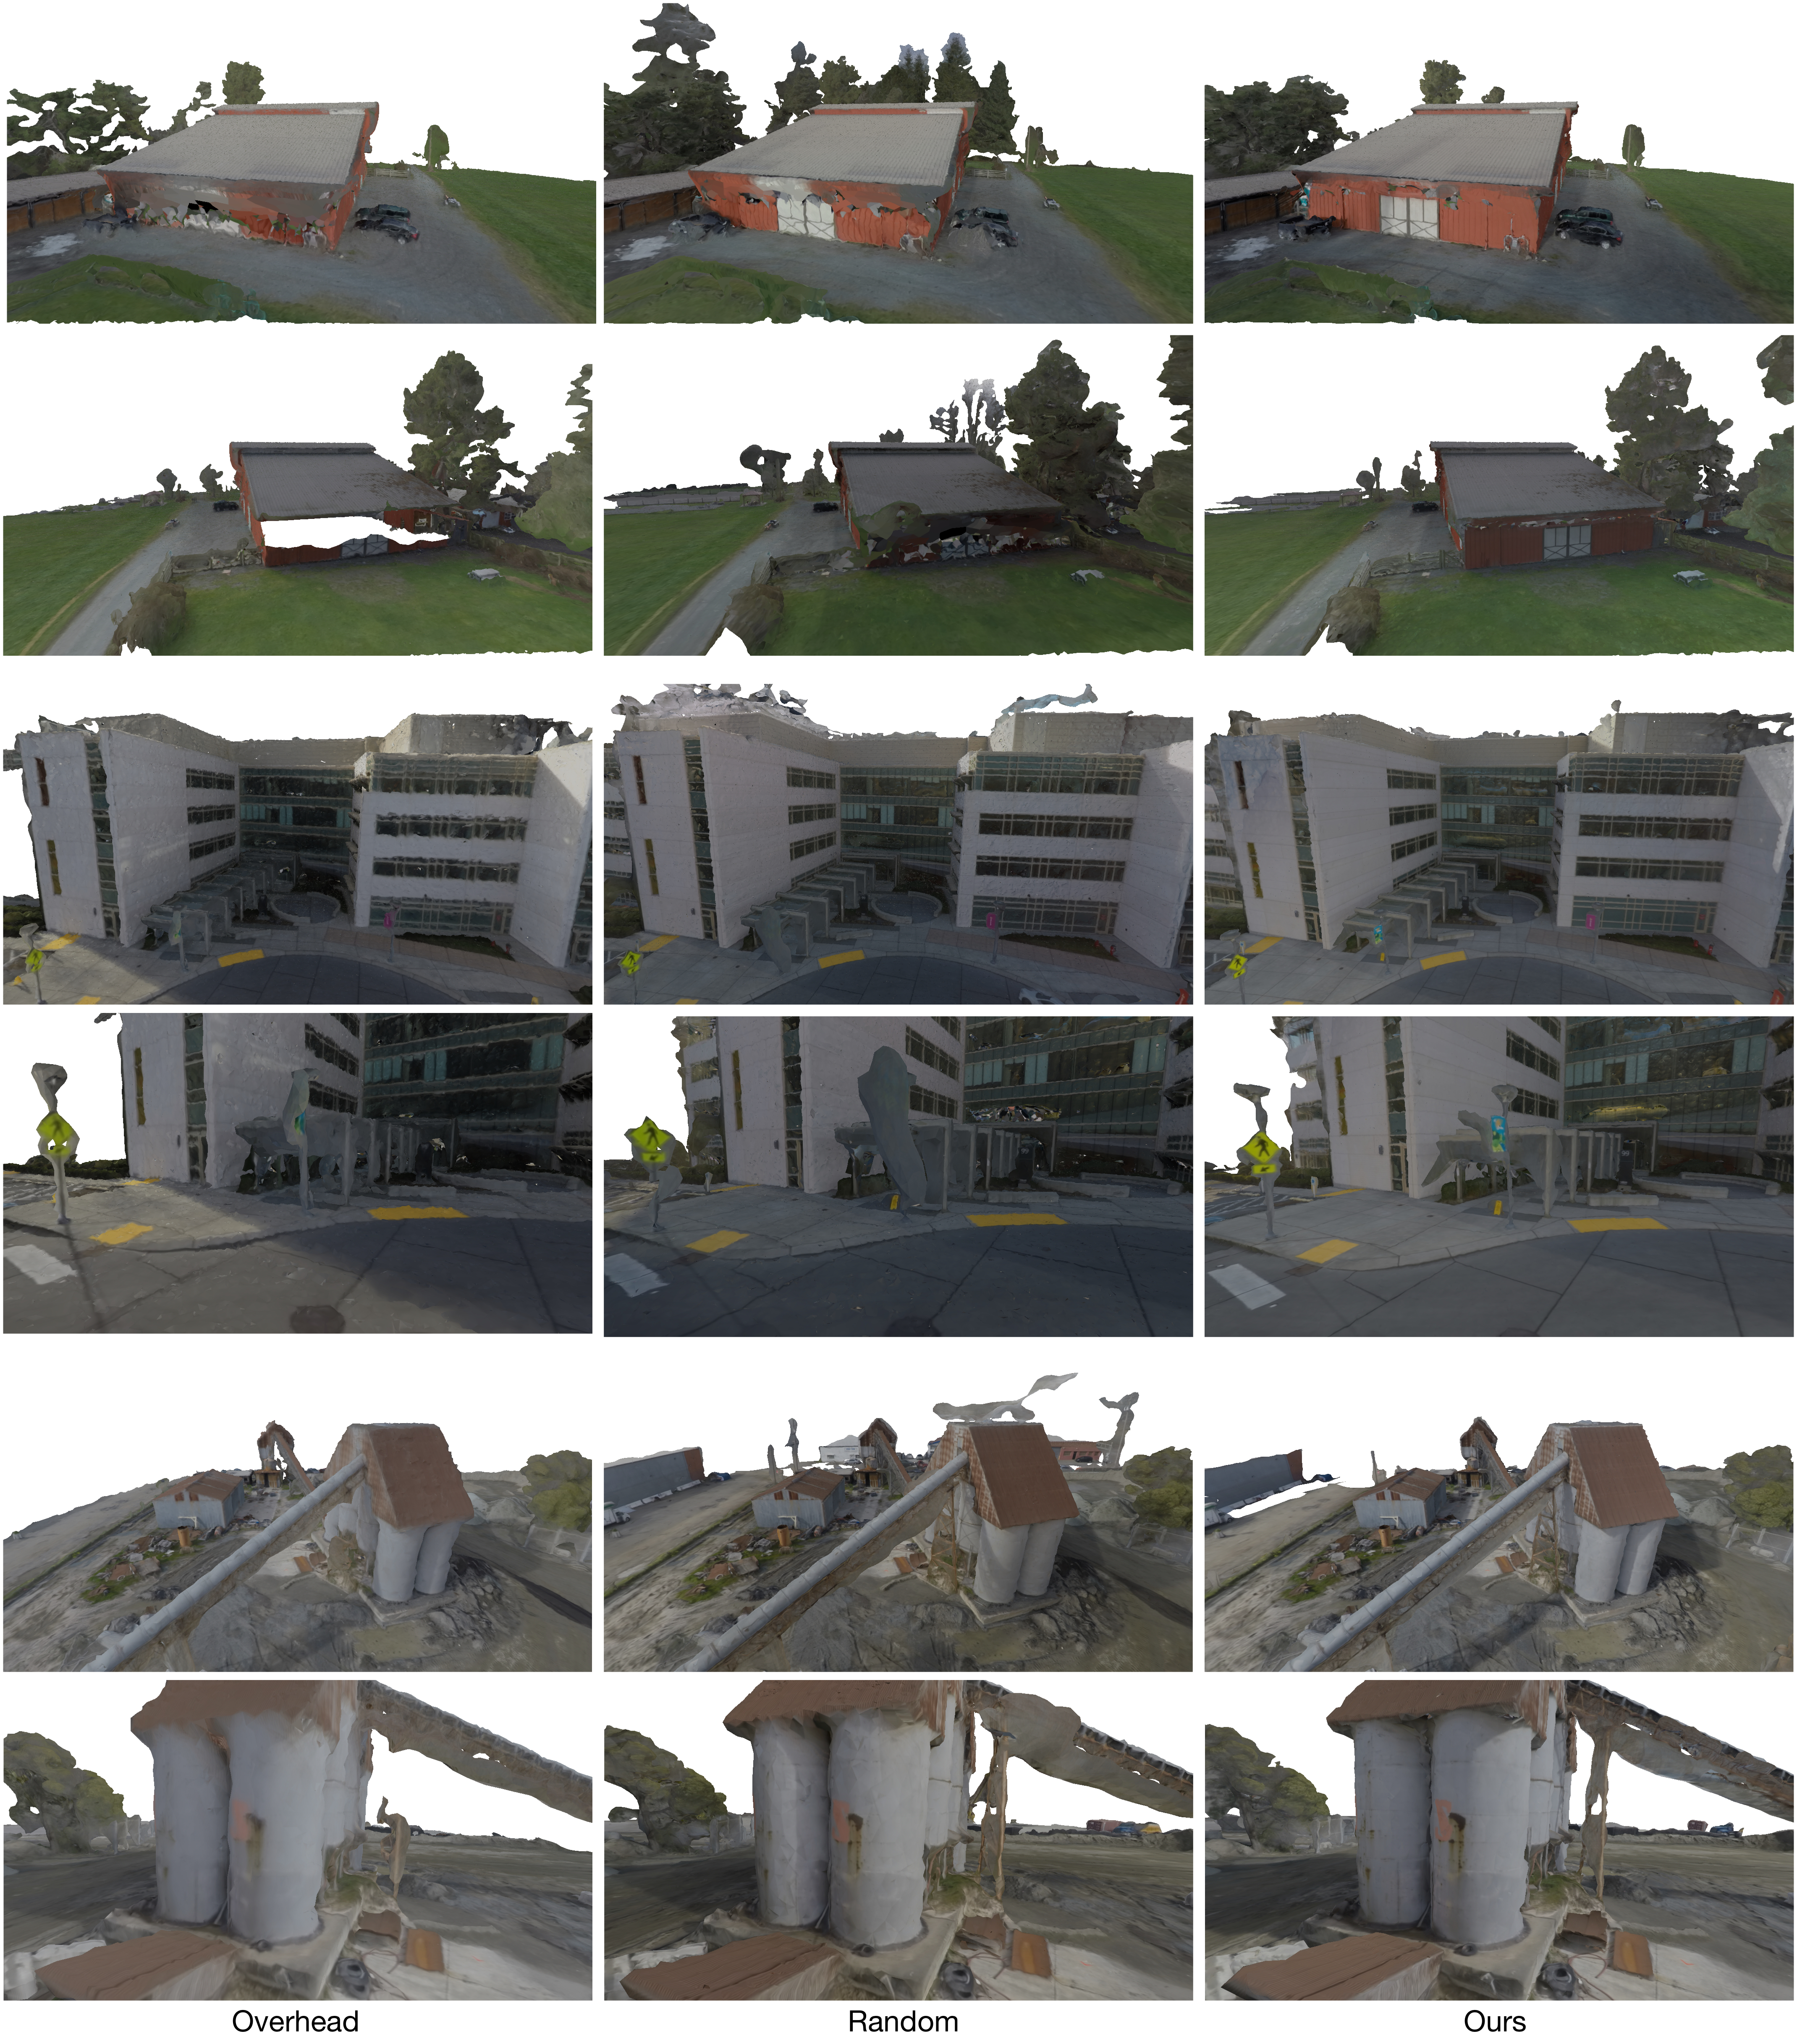
\includegraphics[width=0.99\textwidth]{images/2017_iccv_supplementary/results_supplementary.jpg}
\end{center}
\caption{
Qualitative comparison of the 3D reconstructions produced by overhead, random, and our trajectories for three real-world scenes.
Our reconstructions contain noticeably fewer artifacts than the baseline reconstructions.
In all our experiments, we control for the flight time, battery consumption, number of images, and quality settings used in the 3D reconstruction.
Best viewed digitally at high resolution.
\vspace{-6pt}
}
\label{fig:results_supplementary}
\end{figure*}



\chapter{Conclusions}

\prefacesection{Acknowledgments}

This dissertation would have been impossible without the help and support of many people.
I am indebted to all of you, and I am delighted to take this opportunity to recognize the positive impact that all of you have had on my life.

I want to begin by thanking the world's greatest advisor, Pat Hanrahan.
You took me on as your student even though I didn't know what I was doing.
You were so patient with me, and you gave me the time I needed to grow into a good student and an independent researcher.
You gave me the freedom to choose my own research directions.
You spent countless hours with me discussing research ideas, and you provided a seemingly endless supply of helpful feedback on paper drafts and talks.
Your guidance and mentorship have been transformative.

I want to thank Fr{\'e}do Durand and Doug James for serving on my dissertation reading committee.
Fr{\'e}do's notes on writing became my bible during my graduate studies, and I especially appreciate the advice Doug gave me about choosing research problems back at Harvard.
Doug and Fr{\'e}do also provided very helpful and detailed feedback on an early version of my job talk. I want to thank Ron Fedkiw and Stephen Boyd for serving on my dissertation defense committee.
Ron's lab was an intellectual home-away-from-home, and I especially enjoyed all of our lively discussions over the years.
I also heard a rumor that Ron rescued my Stanford application from the reject pile -- thank you.
Stephen's textbooks, classes, online lectures, and office hours were always incredibly educational, both in their substance and style.

I want to thank Hanspeter Pfister.
You were the first person to give me a chance to do research outside my home town.
This opportunity changed my life.
I also want to thank John Owens.
You were the first person I ever met at an academic conference, and have been an exemplary role model and continuing source of inspiration ever since.
I especially appreciate your guidance on re-applying to Stanford, which undoubtedly changed my life for the better.
While you were hosting me for a visit at UC Davis, Shubho Sengupta offered a comfy couch to sleep on, and Andrew Davidson gave me a lift to the airport -- thank you.

I want to thank my recommenders:
Adam Finkelstein, Pat Hanrahan, Doug James, John Owens, Hanspeter Pfister, and Sudipta Sinha.
You all submitted a gazillion recommendation letters on my behalf, and were all so incredibly generous with your time.
Discussing research ideas with Adam was always fun and inspirational.
Sudipta introduced me to submodular functions, which had a big impact on this dissertation, and our whiteboard sessions were some of my favorite experiences in graduate school.

During my time at Stanford, I benefited from many other amazing mentors.
Floraine Berthouzoz was an incredible role model and collaborator.
Our discussions were always fun and inspirational, and our late-night paper editing sessions had a lasting impact on me.
I wish I could have shared more of the ideas in this dissertation with you.
Russ Tedrake carefully replied to so many of my emails, and his online lectures inspired much of the work in this dissertation.
Stefanie Jegelka's tutorials and online lectures also directly inspired the work in this dissertation.
Mykel Kochenderfer and Silvio Savarese agreed to participate in my qualifying exam -- thank you.
Vladlen Koltun and Ge Wang agreed to take me on as a rotation student even though I didn't know what I was doing.
Maneesh Agrawala, Michael Bernstein, Kayvon Fatahalian, Doug James, James Landay, and Mac Schwager provided valuable ongoing advice, and were all extremely generous with their time.
Wilmot Li provided detailed and helpful feedback on an early paper draft.
Working with John Owens and David Luebke at Udacity was a once-in-a-lifetime opportunity.
Working closely with Frank Dellaert at Skydio was incredibly fun and educational.
Debadeepta Dey, Neel Joshi, Ashish Kapoor, Shital Shah, and Sudipta Sinha at Microsoft Research were all fantastic collaborators.

I couldn't have asked for better friends, colleagues, and labmates at Stanford.
Niels Joubert immediately became a close collaborator and an even closer friend.
Indeed, many of the ideas in this dissertation were conceived during our memorable late-night coding sessions.
Anh Truong and Jane E quickly became trusted confidants and valued collaborators.
I especially appreciate all of Anh's fantastic work on our 3D scanning project, and Jane's work to narrate one of our supplementary videos.
Gilbert Bernstein, Zach DeVito, James Hegarty, Matt Fisher, Sharon Lin, Jonathan Ragan-Kelley, Daniel Ritchie, Manolis Savva, Lingfeng Yang, and Yi-Ting Yeh were fantastic colleagues and role models.
I especially want to thank Zach and Jonathan for putting up with it when I would sleep in their office -- you were doing me a bigger favor than you realize.
Ross Daly and Mackenzie Leake helped to prepare figures and supplementary materials for a paper at the last possible nanosecond.
Maxine Lim created several figures that appear in this dissertation.
Ali Alkhatib, Will Crichton, Abe Davis, Jingyi Li, Alex Poms, and Jerry Talton provided a ton of helpful feedback on various talks and paper drafts.
I especially appreciated all the conversations, coding sessions, and late-night snacks with Ed Quigley and Winnie Lin.
Justin Johnson was the world's greatest group project partner -- thank you for being so patient with me.
Enzo Busseti and Okke Schrijvers became life-long friends.

I also had the opportunity to work with many wonderful friends, colleagues, and labmates at Harvard.
Won-Ki Jeong was willing to work with me even though I didn't know what I was doing.
Bjoern Andres, Verena Kaynig-Fittkau, and Amelio Vazquez-Reina inspired me to learn everything I could about optimization.
Moritz Baecher, Kevin Dale, Kalyan Sunkavalli, and Justin Thaler became close friends.
I especially want to thank Kevin and Kalyan for generously sharing their accommodations at SIGGRAPH with me -- you were doing me a bigger favor than you realize.  
Johanna Beyer, Nicolas Bonneel, Michelle Borkin, Cris Cecka, Markus Hadwiger, Daniel Haehn, Ray Jones, Bobby Kasthuri, Seymour Knowles-Barley,  Jeff Lichtman, Miriah Meyer, Nicolas Pinto, and Amanda Randles were wonderful collaborators and role models.

I appreciate the technical and administrative support I received throughout my graduate studies.
Weichao Qiu provided extensive technical support with his incredibly useful UnrealCV Python library.
Jim Piavis and Ross Robinson provided valuable expertise as safety pilots, and Don Gillett granted us permission to 3D scan his barn.
I am also thankful for the support I received from the exceptional administrative staff in the Stanford Computer Science Department.
In particular, Helen Buendicho, Chris Downey, Jam Kiattinant, Andrea Kuduk, Jillian Lentz, Monica Niemiec, and Jay Subramanian have all gone out of their way to help me countless times.

The work in this dissertation was funded by NSERC and a generous grant from Google.
3DRobotics generously donated the drone hardware we used throughout this dissertation, and granted us permission to 3D scan their industrial scene.
Thank you.

Moving beyond academia, I am grateful for the people in my personal life that have helped and supported me throughout my graduate career.
In Calgary, Chelsea Leishman and the rest of Leishman family always believed in me.
Rob Faust remains a life-long friend, and is still the best DJ partner on the planet.
In Boston, Eric Baczuk and Simon Scheider were always great workout buddies, and I always enjoyed our endless conversations at Chipotle.
When I got to Stanford, I was fortunate to navigate the challenges and adventures of graduate student life alongside Okke Schrijvers.
Shannon Hoban and the rest of the Hoban family, Danielle Radin, Nikil and Tara Viswanathan, Ian Winters, and Brooke Wright all helped to make Stanford feel like home.
Dinner parties with Greg Benedict and Leah Meth were always welcome study breaks.
Cedar House in Berkeley was a home-away-from-home, and Iris Corey, Hannah Marshall, and Armin Samii immediately became close friends.
I especially appreciate Armin for hosting me when I was considering attending UC Berkeley for graduate school, and I want to thank Armin and Dave Jackson for lending me their spare hotel room at SIGGRAPH.

Throughout my graduate studies, I had the opportunity to meet many wonderful housemates.
In particular, Heather and Zac Altman, Katie Ballenger, Caroline Beaudon, Akhila Bettadapur, Nigel Kooreman, Felipe Pincheira, Jessica Schrouff, Gustavo Schwenkler, Alex and Andreas Zoellner quickly became close friends, and all made the Hackmann House a joy to come home to.
Living in the Facebook House was surreal and hilarious thanks to Kai Kuspa.
I was extremely fortunate to live in Hawthorne Manor with  Aladin Corhodzic, Mike D'Amico, Sherif Kassatly, and Ibrahim Toukan.
I experienced so many laughs and wonderful memories with all of you.
I especially appreciate Sherif and Ibrahim for lending me a couple of months of rent at one point -- thank you.
Sherif also did me a huge favor by lending me his old laptop when mine got stolen.

My time at Stanford was undoubtedly more fun because of all the opportunities I had to get in my musical happy place through DJing.
I am thankful for all my friends that made this possible.
Armin Samii hosted the best house party of all time, and trusted me to DJ at it.
Jack Wang at KZSU trusted me to DJ at Stanford football games soon after we met.
Jake Zeller went out of his way to connect me with nightclubs in San Francisco, which ultimately enabled me to open for the Chainsmokers.
Working with Ladidi Gharba was a once-in-a-lifetime opportunity.
I miss you.
Henrik Thorenfeldt trusted me to DJ at the Young Scandinavians Club cabin at Clear Lake.
We quickly became close friends, and Clear Lake became a second family.
Brian Mac immediately became a close friend and trusted DJ partner.

Finally, I want to thank my mom and dad, Judy and Rodger Roberts, for their kind words of support over the years.
And I especially want to thank my brother, Anthony Roberts.
Several times throughout my studies, you loaned me a significant amount of money, and these extraordinary acts of trust enabled me to continue pushing forward.
I would not have been able to complete this dissertation without you.
Thank you.


\appendix

\prefacesection{Acknowledgments}

This dissertation would have been impossible without the help and support of many people.
I am indebted to all of you, and I am delighted to take this opportunity to recognize the positive impact that all of you have had on my life.

I want to begin by thanking the world's greatest advisor, Pat Hanrahan.
You took me on as your student even though I didn't know what I was doing.
You were so patient with me, and you gave me the time I needed to grow into a good student and an independent researcher.
You gave me the freedom to choose my own research directions.
You spent countless hours with me discussing research ideas, and you provided a seemingly endless supply of helpful feedback on paper drafts and talks.
Your guidance and mentorship have been transformative.

I want to thank Fr{\'e}do Durand and Doug James for serving on my dissertation reading committee.
Fr{\'e}do's notes on writing became my bible during my graduate studies, and I especially appreciate the advice Doug gave me about choosing research problems back at Harvard.
Doug and Fr{\'e}do also provided very helpful and detailed feedback on an early version of my job talk. I want to thank Ron Fedkiw and Stephen Boyd for serving on my dissertation defense committee.
Ron's lab was an intellectual home-away-from-home, and I especially enjoyed all of our lively discussions over the years.
I also heard a rumor that Ron rescued my Stanford application from the reject pile -- thank you.
Stephen's textbooks, classes, online lectures, and office hours were always incredibly educational, both in their substance and style.

I want to thank Hanspeter Pfister.
You were the first person to give me a chance to do research outside my home town.
This opportunity changed my life.
I also want to thank John Owens.
You were the first person I ever met at an academic conference, and have been an exemplary role model and continuing source of inspiration ever since.
I especially appreciate your guidance on re-applying to Stanford, which undoubtedly changed my life for the better.
While you were hosting me for a visit at UC Davis, Shubho Sengupta offered a comfy couch to sleep on, and Andrew Davidson gave me a lift to the airport -- thank you.

I want to thank my recommenders:
Adam Finkelstein, Pat Hanrahan, Doug James, John Owens, Hanspeter Pfister, and Sudipta Sinha.
You all submitted a gazillion recommendation letters on my behalf, and were all so incredibly generous with your time.
Discussing research ideas with Adam was always fun and inspirational.
Sudipta introduced me to submodular functions, which had a big impact on this dissertation, and our whiteboard sessions were some of my favorite experiences in graduate school.

During my time at Stanford, I benefited from many other amazing mentors.
Floraine Berthouzoz was an incredible role model and collaborator.
Our discussions were always fun and inspirational, and our late-night paper editing sessions had a lasting impact on me.
I wish I could have shared more of the ideas in this dissertation with you.
Russ Tedrake carefully replied to so many of my emails, and his online lectures inspired much of the work in this dissertation.
Stefanie Jegelka's tutorials and online lectures also directly inspired the work in this dissertation.
Mykel Kochenderfer and Silvio Savarese agreed to participate in my qualifying exam -- thank you.
Vladlen Koltun and Ge Wang agreed to take me on as a rotation student even though I didn't know what I was doing.
Maneesh Agrawala, Michael Bernstein, Kayvon Fatahalian, Doug James, James Landay, and Mac Schwager provided valuable ongoing advice, and were all extremely generous with their time.
Wilmot Li provided detailed and helpful feedback on an early paper draft.
Working with John Owens and David Luebke at Udacity was a once-in-a-lifetime opportunity.
Working closely with Frank Dellaert at Skydio was incredibly fun and educational.
Debadeepta Dey, Neel Joshi, Ashish Kapoor, Shital Shah, and Sudipta Sinha at Microsoft Research were all fantastic collaborators.

I couldn't have asked for better friends, colleagues, and labmates at Stanford.
Niels Joubert immediately became a close collaborator and an even closer friend.
Indeed, many of the ideas in this dissertation were conceived during our memorable late-night coding sessions.
Anh Truong and Jane E quickly became trusted confidants and valued collaborators.
I especially appreciate all of Anh's fantastic work on our 3D scanning project, and Jane's work to narrate one of our supplementary videos.
Gilbert Bernstein, Zach DeVito, James Hegarty, Matt Fisher, Sharon Lin, Jonathan Ragan-Kelley, Daniel Ritchie, Manolis Savva, Lingfeng Yang, and Yi-Ting Yeh were fantastic colleagues and role models.
I especially want to thank Zach and Jonathan for putting up with it when I would sleep in their office -- you were doing me a bigger favor than you realize.
Ross Daly and Mackenzie Leake helped to prepare figures and supplementary materials for a paper at the last possible nanosecond.
Maxine Lim created several figures that appear in this dissertation.
Ali Alkhatib, Will Crichton, Abe Davis, Jingyi Li, Alex Poms, and Jerry Talton provided a ton of helpful feedback on various talks and paper drafts.
I especially appreciated all the conversations, coding sessions, and late-night snacks with Ed Quigley and Winnie Lin.
Justin Johnson was the world's greatest group project partner -- thank you for being so patient with me.
Enzo Busseti and Okke Schrijvers became life-long friends.

I also had the opportunity to work with many wonderful friends, colleagues, and labmates at Harvard.
Won-Ki Jeong was willing to work with me even though I didn't know what I was doing.
Bjoern Andres, Verena Kaynig-Fittkau, and Amelio Vazquez-Reina inspired me to learn everything I could about optimization.
Moritz Baecher, Kevin Dale, Kalyan Sunkavalli, and Justin Thaler became close friends.
I especially want to thank Kevin and Kalyan for generously sharing their accommodations at SIGGRAPH with me -- you were doing me a bigger favor than you realize.  
Johanna Beyer, Nicolas Bonneel, Michelle Borkin, Cris Cecka, Markus Hadwiger, Daniel Haehn, Ray Jones, Bobby Kasthuri, Seymour Knowles-Barley,  Jeff Lichtman, Miriah Meyer, Nicolas Pinto, and Amanda Randles were wonderful collaborators and role models.

I appreciate the technical and administrative support I received throughout my graduate studies.
Weichao Qiu provided extensive technical support with his incredibly useful UnrealCV Python library.
Jim Piavis and Ross Robinson provided valuable expertise as safety pilots, and Don Gillett granted us permission to 3D scan his barn.
I am also thankful for the support I received from the exceptional administrative staff in the Stanford Computer Science Department.
In particular, Helen Buendicho, Chris Downey, Jam Kiattinant, Andrea Kuduk, Jillian Lentz, Monica Niemiec, and Jay Subramanian have all gone out of their way to help me countless times.

The work in this dissertation was funded by NSERC and a generous grant from Google.
3DRobotics generously donated the drone hardware we used throughout this dissertation, and granted us permission to 3D scan their industrial scene.
Thank you.

Moving beyond academia, I am grateful for the people in my personal life that have helped and supported me throughout my graduate career.
In Calgary, Chelsea Leishman and the rest of Leishman family always believed in me.
Rob Faust remains a life-long friend, and is still the best DJ partner on the planet.
In Boston, Eric Baczuk and Simon Scheider were always great workout buddies, and I always enjoyed our endless conversations at Chipotle.
When I got to Stanford, I was fortunate to navigate the challenges and adventures of graduate student life alongside Okke Schrijvers.
Shannon Hoban and the rest of the Hoban family, Danielle Radin, Nikil and Tara Viswanathan, Ian Winters, and Brooke Wright all helped to make Stanford feel like home.
Dinner parties with Greg Benedict and Leah Meth were always welcome study breaks.
Cedar House in Berkeley was a home-away-from-home, and Iris Corey, Hannah Marshall, and Armin Samii immediately became close friends.
I especially appreciate Armin for hosting me when I was considering attending UC Berkeley for graduate school, and I want to thank Armin and Dave Jackson for lending me their spare hotel room at SIGGRAPH.

Throughout my graduate studies, I had the opportunity to meet many wonderful housemates.
In particular, Heather and Zac Altman, Katie Ballenger, Caroline Beaudon, Akhila Bettadapur, Nigel Kooreman, Felipe Pincheira, Jessica Schrouff, Gustavo Schwenkler, Alex and Andreas Zoellner quickly became close friends, and all made the Hackmann House a joy to come home to.
Living in the Facebook House was surreal and hilarious thanks to Kai Kuspa.
I was extremely fortunate to live in Hawthorne Manor with  Aladin Corhodzic, Mike D'Amico, Sherif Kassatly, and Ibrahim Toukan.
I experienced so many laughs and wonderful memories with all of you.
I especially appreciate Sherif and Ibrahim for lending me a couple of months of rent at one point -- thank you.
Sherif also did me a huge favor by lending me his old laptop when mine got stolen.

My time at Stanford was undoubtedly more fun because of all the opportunities I had to get in my musical happy place through DJing.
I am thankful for all my friends that made this possible.
Armin Samii hosted the best house party of all time, and trusted me to DJ at it.
Jack Wang at KZSU trusted me to DJ at Stanford football games soon after we met.
Jake Zeller went out of his way to connect me with nightclubs in San Francisco, which ultimately enabled me to open for the Chainsmokers.
Working with Ladidi Gharba was a once-in-a-lifetime opportunity.
I miss you.
Henrik Thorenfeldt trusted me to DJ at the Young Scandinavians Club cabin at Clear Lake.
We quickly became close friends, and Clear Lake became a second family.
Brian Mac immediately became a close friend and trusted DJ partner.

Finally, I want to thank my mom and dad, Judy and Rodger Roberts, for their kind words of support over the years.
And I especially want to thank my brother, Anthony Roberts.
Several times throughout my studies, you loaned me a significant amount of money, and these extraordinary acts of trust enabled me to continue pushing forward.
I would not have been able to complete this dissertation without you.
Thank you.


\bibliographystyle{plain}
\bibliography{00_main}

\end{document}
